%!TEX TS-program = xelatex
%!TEX encoding = UTF-8 Unicode

%! xelatex thesis.tex
%! makeindex thesis.nlo -s nomencl.ist -o thesis.nls

\documentclass{hi-thesis} 

\usepackage{ifthen}
\usepackage{float}
\usepackage{morefloats}

\usepackage{footnote}
\usepackage[bottom,perpage,symbol*]{footmisc}

\newcommand{\tcr}[1]{{\color{red} #1}}
\newcommand{\tcb}[1]{{\color{blue} #1}}
\newcommand{\tcg}[1]{{\color{green} #1}}
\newcommand{\Alice}{Alice}
\newcommand{\fullnameAlice}{Adaptive Learning Intelligent Composite rulEs}

\newcommand*\blankpage{%
	\newpage	
	\topskip0pt
	\vspace*{\fill}
	\centering This page is intentionally left blank.
	\vspace{\fill}			
}

 % put your own shorthand declarations in this document
\input{../shorthandCommon}
\bibinput{../papers} % put only your publications here

\newcommand{\printFrontMatter}[1]{
  \ifthenelse{\equal{#1}{true}}{
      % some details about the thesis
\title{\Alice: \fullnameAlice}
\author{Helga Ingimundard\'{o}ttir}

% about the degree
\degree{doctor of philosophy}
\field{Computer Science}
\degreeyear{2015}
\degreemonth{May}

% about the university
\department{School of Engineering and Natural Sciences}
\faculty{Faculty of Industrial Eng., Mechanical Eng. and Computer Science}
\university{University of Iceland}
\universitycity{Reykjav\'{i}k}
\universitycountry{Iceland}

% doctoral committee 
\advisor{Prof. T\'{o}mas Philip R\'{u}narsson}
\advisoraffiliation{Faculty of Engineering, University of Iceland}

\committeeA{Prof. Gunnar Stef\'{a}nsson}
\committeeaffiliationA{Faculty of Physical Sciences, University of Iceland}

\committeeB{Mich\`{e}le Sebag}
\committeeaffiliationB{TAO (INRIA Saclay -- \^{I}le-de-France)}

% opponents
\opponentA{Prof. Darrell Whitley}
\opponentaffiliationA{Colorado State University}

\opponentB{Prof. Mark Schoenauer}
\opponentaffiliationB{Director of research with INRIA Saclay -- 
\^{I}le-de-France}
  
% printing
\printer{H\'{a}sk\'{o}laprent}
\ISBN{978-9979-9807-1-1}
      \maketitle
      \copyrightpage
      \dedicationpage
      \abstractpage % both in English and Icelandic
      \tableofcontents
      \listoffigures
      \addcontentsline{toc}{chapter}{Listing of Figures}
      \listoftables
      \addcontentsline{toc}{chapter}{Listing of Tables}
      \addcontentsline{toc}{chapter}{Listing of Publications}
\chapter*{Listing of Publications}
The thesis is based on the following publications:
\begin{description} 
    \item[Paper \labelcref{InRu11a}] \nameref{InRu11a}
    \item[Paper \labelcref{InRu11b}] \nameref{InRu11b}
    \item[Paper \labelcref{InRu12} ] \nameref{InRu12}
    \item[Paper \labelcref{InRu14} ] \nameref{InRu14}
    \item[Paper \labelcref{InRu15a}] \nameref{InRu15a}
\end{description}

\defcitealias{InRu11a}{Paper \labelcref{InRu11a}}
\defcitealias{InRu11b}{Paper \labelcref{InRu11b}}
\defcitealias{InRu12}{Paper \labelcref{InRu12}}
\defcitealias{InRu14}{Paper \labelcref{InRu14}}
\defcitealias{InRu15a}{Paper \labelcref{InRu15a}}

      %\nomenclature[zcif]{$CIF$}{Cauchy's Integral Formula}                  % first letter Z is for Acronyms 
%\nomenclature[aF]{$F$}{complex function}                               % first letter A is for Roman symbols
%\nomenclature[gp]{$\pi$}{ $\simeq 3.14\ldots$}                         % first letter G is for Greek Symbols
%\nomenclature[gi]{$\iota$}{unit imaginary number $\sqrt{-1}$}          % first letter G is for Greek Symbols
%\nomenclature[gg]{$\gamma$}{a simply closed curve on a complex plane}  % first letter G is for Greek Symbols
%\nomenclature[xi]{$\oint_\gamma$}{integration around a curve $\gamma$} % first letter X is for Other Symbols
%\nomenclature[rj]{$j$}{superscript index}                              % first letter R is for superscripts
%\nomenclature[s0]{$0$}{subscript index}                                % first letter S is for subscripts

% Rice's Framework
\nomenclature[f01]{$\mathcal{P}$}{Problem space or instance space}
\nomenclature[f02]{$\mathcal{F}$}{Feature space, i.e., measurable properties of the instances in $\mathcal{P}$}
\nomenclature[f03]{$\mathcal{A}$}{Algorithm space}
\nomenclature[f04]{$\mathcal{Y}$}{Performance space, i.e., the outcome for $\mathcal{P}$ using an algorithm from $\mathcal{A}$}
\nomenclature[f05]{$Y$}{Mapping for algorithm and feature space onto performance space, i.e., $y=Y(a,\vphi(\vec{x}))\in\mathcal{Y}$ where $Y:\mathcal{A}\times\mathcal{F}\mapsto\mathcal{Y}$}

% JOB SHOP
\nomenclature[j01]{$n$}{number of jobs in shop}
\nomenclature[j02]{$m$}{number of machines in shop}
\nomenclature[j03]{$\mathcal{J}$}{set of jobs, $\{J_1,\dotsc,J_j,\dotsc,J_n\}$}
\nomenclature[j04]{$\mathcal{M}$}{set of machines, $\{M_1,\dotsc,M_a,\dotsc,M_m\}$}
\nomenclature[j05]{$p_{ja}$}{processing time for job $J_j$ on machine $M_a$}
\nomenclature[j06]{$\vsigma_j$}{machine ordering for job $J_j$} 
\nomenclature[j07]{$x_s(j,a)$}{starting time for job $J_j$ on machine $M_a$}
\nomenclature[j08]{$x_f(j,a)$}{finishing time for job $J_j$ on machine $M_a$}
\nomenclature[j09]{$s(a,j)$}{flow between current and previous task on machine $M_a$}
\nomenclature[j10{$\mathcal{R}$}{ready-list of jobs that have unassigned tasks, $\mathcal{R}\subset\mathcal{J}$}
\nomenclature[j11]{$C_{\max}$}{makespan, i.e. maximum completion times for all tasks}
\nomenclature[j12]{$\vchi$}{sequence of dispatches $J_j$ to create (partial) schedule/solution} 
\nomenclature[j13]{$\mathcal{U}(u_1,u_2)$}{uniform distribution from the interval $I=[u_1,u_2]\subset\R$}
\nomenclature[j14]{$\rho$}{percentage relative deviation from optimality}
\nomenclature[j15]{$\ell$}{number of dispatches needed for a complete schedule, $\ell=n\cdot m$}

% ORDINAL REGRESSION 
\nomenclature[o01]{$d$}{number of distinct features, i.e., dimension of $\mathcal{F}$}
\nomenclature[o02]{$N$}{number of problem instances}
\nomenclature[o03]{$\Phi$}{training set}
\nomenclature[o04]{$S$}{preference set}
\nomenclature[o05]{$l$}{size of preference set, $l=\abs{S}$}
\nomenclature[o06]{$\vphi_k$}{feature set, i.e., post-decision state, of a (partial) schedule at time $k$}
\nomenclature[o07]{$\tilde{\vphi}$}{scaled feature set, such that $\tilde{\vphi}_i\in[-1,1]$ for all $i\in\{1,..,d\}$}
\nomenclature[o08]{$\mathcal{O}^{(k)}$}{set of optimal dispatches at time  $k$}
\nomenclature[o09]{$\mathcal{S}^{(k)}$}{set of suboptimal dispatches at time  $k$}
\nomenclature[o10]{$\vec{w}$}{linear weights for features $\vphi$}
\nomenclature[o11]{$h$}{linear classification model, $h(\vec{x})=\inner{\vec{w}}{\vphi(\vec{x})}$}

% SURROGATE MODELLING
\nomenclature[s01]{$\tau$}{Kendall's $\tau$ statistic, i.e., normalised difference in number of concordant and discordant pairs}

% EXPERIMENTAL SETTING
\nomenclature[x01]{$S_b$}{preference set added w.r.t. basic ranking}
\nomenclature[x02]{$S_f$}{preference set added w.r.t. full subsequent ranking}
\nomenclature[x03]{$S_p$}{preference set added w.r.t. partial subsequent ranking}
\nomenclature[x04]{$S_a$}{union of all aforementioned rankings, i.e., $S_{a}=S_b\cup S_f\cup S_p$}
\nomenclature[x05]{$\Phi^{SPT}$}{training data guided by SPT trajectory}
\nomenclature[x06]{$\Phi^{LPT}$}{training data guided by LPT trajectory}
\nomenclature[x07]{$\Phi^{LWR}$}{training data guided by LWR trajectory}
\nomenclature[x08]{$\Phi^{MWR}$}{training data guided by MWR trajectory}
\nomenclature[x09]{$\Phi^{OPT}$}{training data guided by (random) optimum trajectory}
\nomenclature[x10]{$\Phi^{RND}$}{training data guided by a random trajectory}
\nomenclature[x11]{$\Phi^{CMA}$}{training data guided by trajectory using by CMA-ES obtained weights}
\nomenclature[x12]{$\Phi^{ALL}$}{union of all aforementioned trajectories, i.e.,  $S^{ALL}=S^{SPT}\cup S^{LPT}\cup S^{LWR}\cup S^{MWR} \cup S^{OPT} \cup S^{RND} \cup S^{CMA}$}
\nomenclature[x13]{$p^{equal}$}{all preferences sampled equally }
\nomenclature[x14]{$p^{opt}$}{preferences sampled proportional w.r.t. its stepwise optimality}
\nomenclature[x15]{$p^{bcs}$}{preferences sampled reciprocally proportional w.r.t. its stepwise best case scenario of suboptimal dispatches }
\nomenclature[x16]{$p^{wcs}$}{preferences sampled reciprocally proportional w.r.t. its stepwise worst case scenario of suboptimal dispatches }

% SUBSCRIPS AND SUPERSCRIPTS
\nomenclature[y01]{$j$}{refers to job $J_j$}
\nomenclature[y02]{$a$}{refers to machine $M_a$}
\nomenclature[y03]{$k$}{refers to dispatch/time step $k$ for a schedule, $k\in\{1,..,\ell}$}
\nomenclature[y04]{opt}{(known) optimum}
\nomenclature[y05]{sub}{sub-optimum}
\nomenclature[y06]{bks}{best known solution}

% ACRONYMS
\nomenclature[z01]{JSP}{\jsp\ scheduling problem}
\nomenclature[z02]{PFSP}{permutation \fsp\ scheduling problem}
\nomenclature[z03]{DR}{dispatching rule}
\nomenclature[z04]{SDR}{simple priority dispatching rule}
\nomenclature[z05]{CDR}{composite dispatching rule}
\nomenclature[z06]{BDR}{blended dispatching rule}
\nomenclature[z07]{SPT}{shortest processing time}
\nomenclature[z08]{LPT}{largest processing time}
\nomenclature[z09]{LWR}{least work remaining}
\nomenclature[z10]{MWR}{most work remaining}
\nomenclature[z11]{ES}{evolution strategy}
\nomenclature[z12]{CMA}{covariance matrix adaptation}
\nomenclature[z13]{PREF}{linear preference learning model}
      \printnomenclature  
      \addcontentsline{toc}{chapter}{Nomenclature}
      \acknowledgments
  }{}
  \ifthenelse{\equal{#1}{false}}{
    \pagenumbering{roman}
	  \listoftodos
	  
	  \tableofcontents
	  \listoffigures
	  \addcontentsline{toc}{chapter}{Listing of Figures}
	  \listoftables
	  \addcontentsline{toc}{chapter}{Listing of Tables}
	  %\nomenclature[zcif]{$CIF$}{Cauchy's Integral Formula}                  % first letter Z is for Acronyms 
%\nomenclature[aF]{$F$}{complex function}                               % first letter A is for Roman symbols
%\nomenclature[gp]{$\pi$}{ $\simeq 3.14\ldots$}                         % first letter G is for Greek Symbols
%\nomenclature[gi]{$\iota$}{unit imaginary number $\sqrt{-1}$}          % first letter G is for Greek Symbols
%\nomenclature[gg]{$\gamma$}{a simply closed curve on a complex plane}  % first letter G is for Greek Symbols
%\nomenclature[xi]{$\oint_\gamma$}{integration around a curve $\gamma$} % first letter X is for Other Symbols
%\nomenclature[rj]{$j$}{superscript index}                              % first letter R is for superscripts
%\nomenclature[s0]{$0$}{subscript index}                                % first letter S is for subscripts

% Rice's Framework
\nomenclature[f01]{$\mathcal{P}$}{Problem space or instance space}
\nomenclature[f02]{$\mathcal{F}$}{Feature space, i.e., measurable properties of the instances in $\mathcal{P}$}
\nomenclature[f03]{$\mathcal{A}$}{Algorithm space}
\nomenclature[f04]{$\mathcal{Y}$}{Performance space, i.e., the outcome for $\mathcal{P}$ using an algorithm from $\mathcal{A}$}
\nomenclature[f05]{$Y$}{Mapping for algorithm and feature space onto performance space, i.e., $y=Y(a,\vphi(\vec{x}))\in\mathcal{Y}$ where $Y:\mathcal{A}\times\mathcal{F}\mapsto\mathcal{Y}$}

% JOB SHOP
\nomenclature[j01]{$n$}{number of jobs in shop}
\nomenclature[j02]{$m$}{number of machines in shop}
\nomenclature[j03]{$\mathcal{J}$}{set of jobs, $\{J_1,\dotsc,J_j,\dotsc,J_n\}$}
\nomenclature[j04]{$\mathcal{M}$}{set of machines, $\{M_1,\dotsc,M_a,\dotsc,M_m\}$}
\nomenclature[j05]{$p_{ja}$}{processing time for job $J_j$ on machine $M_a$}
\nomenclature[j06]{$\vsigma_j$}{machine ordering for job $J_j$} 
\nomenclature[j07]{$x_s(j,a)$}{starting time for job $J_j$ on machine $M_a$}
\nomenclature[j08]{$x_f(j,a)$}{finishing time for job $J_j$ on machine $M_a$}
\nomenclature[j09]{$s(a,j)$}{flow between current and previous task on machine $M_a$}
\nomenclature[j10{$\mathcal{R}$}{ready-list of jobs that have unassigned tasks, $\mathcal{R}\subset\mathcal{J}$}
\nomenclature[j11]{$C_{\max}$}{makespan, i.e. maximum completion times for all tasks}
\nomenclature[j12]{$\vchi$}{sequence of dispatches $J_j$ to create (partial) schedule/solution} 
\nomenclature[j13]{$\mathcal{U}(u_1,u_2)$}{uniform distribution from the interval $I=[u_1,u_2]\subset\R$}
\nomenclature[j14]{$\rho$}{percentage relative deviation from optimality}
\nomenclature[j15]{$\ell$}{number of dispatches needed for a complete schedule, $\ell=n\cdot m$}

% ORDINAL REGRESSION 
\nomenclature[o01]{$d$}{number of distinct features, i.e., dimension of $\mathcal{F}$}
\nomenclature[o02]{$N$}{number of problem instances}
\nomenclature[o03]{$\Phi$}{training set}
\nomenclature[o04]{$S$}{preference set}
\nomenclature[o05]{$l$}{size of preference set, $l=\abs{S}$}
\nomenclature[o06]{$\vphi_k$}{feature set, i.e., post-decision state, of a (partial) schedule at time $k$}
\nomenclature[o07]{$\tilde{\vphi}$}{scaled feature set, such that $\tilde{\vphi}_i\in[-1,1]$ for all $i\in\{1,..,d\}$}
\nomenclature[o08]{$\mathcal{O}^{(k)}$}{set of optimal dispatches at time  $k$}
\nomenclature[o09]{$\mathcal{S}^{(k)}$}{set of suboptimal dispatches at time  $k$}
\nomenclature[o10]{$\vec{w}$}{linear weights for features $\vphi$}
\nomenclature[o11]{$h$}{linear classification model, $h(\vec{x})=\inner{\vec{w}}{\vphi(\vec{x})}$}

% SURROGATE MODELLING
\nomenclature[s01]{$\tau$}{Kendall's $\tau$ statistic, i.e., normalised difference in number of concordant and discordant pairs}

% EXPERIMENTAL SETTING
\nomenclature[x01]{$S_b$}{preference set added w.r.t. basic ranking}
\nomenclature[x02]{$S_f$}{preference set added w.r.t. full subsequent ranking}
\nomenclature[x03]{$S_p$}{preference set added w.r.t. partial subsequent ranking}
\nomenclature[x04]{$S_a$}{union of all aforementioned rankings, i.e., $S_{a}=S_b\cup S_f\cup S_p$}
\nomenclature[x05]{$\Phi^{SPT}$}{training data guided by SPT trajectory}
\nomenclature[x06]{$\Phi^{LPT}$}{training data guided by LPT trajectory}
\nomenclature[x07]{$\Phi^{LWR}$}{training data guided by LWR trajectory}
\nomenclature[x08]{$\Phi^{MWR}$}{training data guided by MWR trajectory}
\nomenclature[x09]{$\Phi^{OPT}$}{training data guided by (random) optimum trajectory}
\nomenclature[x10]{$\Phi^{RND}$}{training data guided by a random trajectory}
\nomenclature[x11]{$\Phi^{CMA}$}{training data guided by trajectory using by CMA-ES obtained weights}
\nomenclature[x12]{$\Phi^{ALL}$}{union of all aforementioned trajectories, i.e.,  $S^{ALL}=S^{SPT}\cup S^{LPT}\cup S^{LWR}\cup S^{MWR} \cup S^{OPT} \cup S^{RND} \cup S^{CMA}$}
\nomenclature[x13]{$p^{equal}$}{all preferences sampled equally }
\nomenclature[x14]{$p^{opt}$}{preferences sampled proportional w.r.t. its stepwise optimality}
\nomenclature[x15]{$p^{bcs}$}{preferences sampled reciprocally proportional w.r.t. its stepwise best case scenario of suboptimal dispatches }
\nomenclature[x16]{$p^{wcs}$}{preferences sampled reciprocally proportional w.r.t. its stepwise worst case scenario of suboptimal dispatches }

% SUBSCRIPS AND SUPERSCRIPTS
\nomenclature[y01]{$j$}{refers to job $J_j$}
\nomenclature[y02]{$a$}{refers to machine $M_a$}
\nomenclature[y03]{$k$}{refers to dispatch/time step $k$ for a schedule, $k\in\{1,..,\ell}$}
\nomenclature[y04]{opt}{(known) optimum}
\nomenclature[y05]{sub}{sub-optimum}
\nomenclature[y06]{bks}{best known solution}

% ACRONYMS
\nomenclature[z01]{JSP}{\jsp\ scheduling problem}
\nomenclature[z02]{PFSP}{permutation \fsp\ scheduling problem}
\nomenclature[z03]{DR}{dispatching rule}
\nomenclature[z04]{SDR}{simple priority dispatching rule}
\nomenclature[z05]{CDR}{composite dispatching rule}
\nomenclature[z06]{BDR}{blended dispatching rule}
\nomenclature[z07]{SPT}{shortest processing time}
\nomenclature[z08]{LPT}{largest processing time}
\nomenclature[z09]{LWR}{least work remaining}
\nomenclature[z10]{MWR}{most work remaining}
\nomenclature[z11]{ES}{evolution strategy}
\nomenclature[z12]{CMA}{covariance matrix adaptation}
\nomenclature[z13]{PREF}{linear preference learning model}	  
	  \printnomenclature  
	  \addcontentsline{toc}{chapter}{Nomenclature}
	  
	  % Main matter
	  \cleardoublepage
	  \pagestyle{fancy} \setcounter{page}{1} \pagenumbering{arabic}
	  \normalsize
	  
	  \cfoot{Draft -- \today}
  }{}
  \onehalfspacing
}
\newcommand{\printBackMatter}[1]{
  % Back matter
  \singlespacing
  \clearpage
  
  \HeaderQuote{A cat may look at a king. I've read that in some book, but I don't remember where.}{Alice}

  \bibliographystyle{abbrvnat} 
  \bibliography{../references}
  \addcontentsline{toc}{chapter}{References}
  \appendix
  \HeaderQuote{Sentence first -- verdict afterwards.}{The Queen}

\chapter{Problem Structure}\label{ch:problemstructure} 

%\begin{abstract} 
%Many heuristic methods have been proposed for the \jsp\ scheduling problem. Different solution methodologies outperform other depending on the particular problem instance under consideration. Therefore, one is interested in knowing how the instances differ in structure and determine when a particular heuristic solution is likely to fail and explore in further detail the causes. In order to achieve this, we seek to characterise features for different difficulties. Preliminary experiments show there are different significant features that distinguish between easy and hard \jsp\ problem, and that they vary throughout the scheduling process. 
%The insight attained by investigating the relationship between problem structure and heuristic performance can undoubtedly lead to better heuristic design that is tailored to the data distribution under consideration.
%\end{abstract}


\FirstSentence{P}{roblem structure and heuristic effectiveness} are closely intertwined. When investigating the relation between the two, one can research what \citet{Corne10} call \emph{footprints} in instance space, which is an indicator how an algorithm generalises over a given instance space. This sort of investigation has also been conducted by \citet{Pfahringer00} under the alias \emph{landmarking}. 
% quote Corne10: ``such a footprint indicates how an algorithm's comparative performance generalises in instance space''
% quote Katie2009: ``Landmarking tries to directly characterise a domain by relating the performance to some learners -- the landmarkers -- to the performance of some other algorithm.''
From experiments performed by \citeauthor{Corne10}, it is evident that one-algorithm-for-all problem instances is not ideal, in accordance with no free lunch theorem \citep{Wolpert97nofree}. An algorithm may be favoured for its best overall performance, however it is rarely the best algorithm available over various subspaces of the instance space.
Therefore, when comparing different algorithms one needs to explore how they perform w.r.t. the instance space, i.e., their footprint. That is to say, one can look at it as finding which footprints correspond to a subset of the instance space that works \emph{well} for a given algorithm, and similarly finding which footprints correspond to a subset of the instance space that works \emph{poorly} for a given algorithm. 

In the context of \jsp\ this corresponds to finding \emph{good} (makespan close to its optimum)  and \emph{bad} (makespan far off its optimum) schedules. Note, good and bad schedules are interchangeably referred to as \emph{easy} and \emph{hard} schedules (pertaining to the manner they are achieved), respectively. 

\citet{SmithMilesLion5} also investigate algorithm performance in instance space using footprints. The main difference between \citeauthor{Corne10} and \citeauthor{SmithMilesLion5} is how they discretise the instance space. In the case of \citeauthor{Corne10} they use \jsp\ and discretise manually between different problem instances; on one hand w.r.t. processing times, e.g.,  $\vec{p}\sim \mathcal{U}(10,20)$ versus $\vec{p}\sim \mathcal{U}(20,30)$ etc., and on the other hand w.r.t. number of jobs, $n$. 
They warn that footprinting can be uneven, so great care needs to be taken in how to discretise the instance space into subspaces. 
On the other hand, \citeauthor{SmithMilesLion5} use a completely automated approach. Using timetabling instances, they implement a self-organizing map to group similar problem instances together, that were both real world instances and synthetic ones using different problem generators. 

Going back to the \jsp\ paradigm, then the interaction between processing time distribution and its permutation is extremely important, because it introduces hidden properties in the data structure making it \emph{easy} or \emph{hard} to schedule for the given algorithm. These underlying characteristics, i.e., features, define its data structure. A more sophisticated way of discretising the instance space is grouping together problem instances that show the same kind of feature behaviour, especially given the fact the learning models in \cref{ch:prefmodels} will be heavily based on feature pairs. Thereby making it possible to infer what sort of feature behaviour distinguishes  between \emph{good} and \emph{bad} schedules. 

In \citet{InRu12}, a single problem generator was used to create  $N=1,500$ synthetic $6\times6$ \jsp\ problem instances, where $\vec{p}\sim\mathcal{U}(1,200)$ and $\vsigma$ was a random permutation. The experimental study showed that MWR works either well or poorly on a subset of the instances, in fact 18\% and 16\% of the instances were classified as \emph{easy} and \emph{hard} for MWR, respectively. 
Since the problem instances were na\"{i}vely generated, not to mention given the high variance of the data distribution, it is intuitive that there are some inherent structural qualities that could explain this difference in performance. The experimental study investigated the feature behaviours for these two subsets, namely, the easy and hard problem instances. For some features, the trend was more or less the same, which are explained by the common denominating factor, that all instances were sampled from the same problem generator. Whereas, those features that were highly correlated with the end-result, i.e., the final makespan, which determined if an instance was labelled easy or hard, then the significant features varied greatly between the two difficulties, which imply the inherent difference in data structure. 
Moreover, the study in gives support to that random problem instance generators are \emph{too} general and might not suit real-world applications. \citet{Whitley} argue that problem instance generator should be more structured, since real-world manufacturing environment is not completely random, but rather structured, e.g.,  job's tasks can be correlated or machines in the shop. \citeauthor{Whitley} propose a problem instance generator that relates to real-world \fsp\ attributes, albeit not directly modelled after real-world \fsp\ due to the fact that deterministic $Fm||C_{\max}$ is seldom directly applicable in practice \citep{Dudek92}. This is why \fjc{n}{m}, \fmc{n}{m} and \fmxc{n}{m} are also taken into consideration in \cref{ch:genprobleminstances} as they are an attempt to mimic the real-world characteristics of \fsp.

It is interesting to know if the difference in the structure of the schedule is time dependent, e.g.,  is there a clear time of divergence within the scheduling process? 
Moreover, investigation of how sensitive is the difference between two sets of features, e.g.,  can two schedules with similar feature values yield completely contradictory outcomes (i.e. one poor and one good schedule)? Or will they more or less follow the their predicted trend? If the latter is the prevalent case, then these instances need to be segregated and each having their own learning algorithm implemented, for a meaningful outcome overall.  
This also, essentially, answers the question of whether  it is in fact feasible to discriminate between \emph{good} and \emph{bad} schedules using the currently selected features as a measure. If results are contradictory, it is an indicator the features selected are not robust enough to capture the essence of the data structure and some key features are missing from the feature set that could be able to discriminate between \emph{good} and \emph{bad} schedules. 
Additionally, there is also the question of how can one define ``similar'' schedules, and what measures should be used? This \lcnamecref{ch:problemstructure} describes some preliminary experiments with the aim of investigating the feasibility of finding distinguishing features corresponding to \emph{good} and \emph{bad} schedules in \jsp. To summarise:
\begin{inparaenum}[(a)]
	\item How to define problem difficulty? 
	\item Is there a time of divergence?
	\item What are ``similar'' schedules?
	\item Do similar features yield contradictory outcomes?
	\item Are extra features needed? 
	And \item what can be learned from feature behaviour?
\end{inparaenum}

Instead of searching through a large set of algorithms  and determining which algorithm is the most suitable for a given subset of the instance space, i.e., creating an algorithm portfolio, as is generally the focus in the current literature \citep{SmithMilesLion3,SmithMilesLion5,Corne10}, the focus of the experimental study in \cref{sec:diff:jrnd,sec:diff:jrndn,sec:diff:frnd,sec:diff:frndn,sec:diff:fjc,sec:diff:fmc,sec:diff:fmxc} 
(each corresponding to a given problem space from \cref{ch:genprobleminstances})
is rather on few simple algorithms, here the SDRs described in \cref{sec:SDR}, and understanding \emph{how} they work on the instance space, similar to \citet{Whitley}, who analyse the fitness landscape of several problem classes for a fixed algorithm. 
Note, figures and tables that accompany this \lcnamecref{ch:problemstructure} are mostly located in \cref{app:problemstructure}.


\section{Distribution difficulty w.r.t. SDRs}
Depending on the data distribution, dispatching rules perform differently. Take for instance the common single-based priority dispatching rules; SPT, LPT, LWR and MWR (cf. \cref{sec:SDR}). 
A box-plot for \fullnamerho, for all problem spaces in \cref{ch:genprobleminstances} are depicted in \cref{fig:SDR:boxplot}. 
As one can see, there is a staggering difference between the interaction of SDRs and their problem space. MWR is by far the best out of the four SDRs inspected for \JSP\ -- not only does it reach the known optimum most often but it also has the lowest worst-case factor from optimality. Similarly LWR for \FSP.
Although the same processing time distribution is used, there are some inherent structure in which MWR and LWR can exploit for \JSP\ and  \FSP, respectively, whereas the other SDRs cannot. However, \emph{all} of these dispatching rules are considered good and commonly used in practice and no one is better than the rest \citep{Haupt89}, it simply depends on the data distribution at hand. This indicates that some distributions are harder than others, and these \JSP\ problem generators simply favours MWR, whereas the \FSP\ problem generators favours LWR. 

\section{Experimental settings}
% Katie orðar: A correlation analysis between the feature space and the performance space was conducted across all 1,500 problem instances revealed that instance features that appear to correlate (linearly) with heuristic performance are $phi(?)$ (correlation $=-0.59$) and $phi(?)$ (correlation $=0.44$). None of the other instance features appear to have a linear relationship with algorithmic performance.

The main focus is on knowing \emph{when} during the scheduling process easy and hard problems diverge and explore in further detail \emph{why} they diverged. Rather than visualising high-dimensional data projected onto two dimensional space (as was the focus in \cite{SmithMilesLion5} with self-organising maps), instead appropriate statistical tests with a significance level $\alpha=0.05$ is applied to determine if there is any difference between different data distributions. For this the two-sample Kolmogorov–Smirnov test (K-S test) is used to determine whether two underlying one-dimensional probability distributions differ. 
Furthermore, in order to find defining characteristics for easy or hard problems, a (linear) correlation is computed between features to the resulting \namerho.

Note, when inspecting any statistical difference between data distribution of the features on a step by step basis, the features at step $k+1$ are of course dependant on all previous $k$ steps. This results in repetitive statistical testing, therefore a Bonferroni adjustment is used to counteract the multiple comparisons, i.e., each stepwise comparison has the significant level $\alpha_k=\frac{\alpha}{\ell}$, and thus maintaining the $\sum_{k=1}^{\ell}\alpha_k=\alpha$ significance level.

\section{Defining `easy' versus `hard' schedules}\label{sec:diff:easyhard}
It's relatively ad-hoc how to define what makes a schedule difficult. Intuitively, it's logical to use the schedule's objective to define it directly, i.e., inspecting \fullnamerho. Moreover, since the SDRs from \cref{sec:SDR} will be used throughout as a benchmark for subsequent models, the quantiles for \namerho, using the SDRs on their training set will be used to differentiate between easy and hard scheduling problems. In particular, the classification is defined as follows, 
\begin{description}
	\item[Easy] schedules belong to the first quantile, i.e., \hfill \\
	\begin{equation}\label{eq:easy}
		\mathcal{E}(a):=\{\vec{x}\;|\;\rho=Y(a,\vec{x})<\rho^{\text{1st. Qu.}}\}
	\end{equation} 
	\item[Hard] schedules belong to the third quantile, i.e., \hfill \\
	\begin{equation}\label{eq:hard}
		\mathcal{H}(a):=\{\vec{x}\;|\;\rho=Y(a,\vec{x})>\rho^{\text{3rd. Qu.}}\}
	\end{equation} 
\end{description}
where $\vec{x}\in\mathcal{P}_{\text{train}}$ for a given dispatching rule $a\in\mathcal{A}:=\{\text{SPT,~LPT,~LWR,~MWR}\}$.

\Cref{tbl:easyhard:quantile} reports the first and third quantiles for each problem space, i.e., the cut-off values that determine the SDRs difficulty, whose division, defined as percentage of problem instances, i.e., 
\begin{equation}\label{eq:easyhard:cnt}
	\frac{\abs{\mathcal{E}(a)}}{N_{\text{train}}} \cdot 100\%
	\quad \text{and} \quad 
	\frac{\abs{\mathcal{H}(a)}}{N_{\text{train}}}\cdot 100\%
\end{equation}
for each $a\in\mathcal{A}$, are given in \cref{tbl:easyhard:cnt:6x5,tbl:easyhard:cnt:10x10}, respectively. 

\section{Consistency of problem instances}
The intersection of pairwise SDRs being simultaneously easy or hard are given in \cref{tbl:easy:cnt:6x5,tbl:easy:cnt:10x10,tbl:hard:cnt:6x5,tbl:hard:cnt:10x10}, i.e., 
\begin{equation}\label{eq:easyorhard:cnt}
	\frac{\abs{\mathcal{E}(a_i)\cap \mathcal{E}(a_j) }}{N_{\text{train}}} \cdot 100\%
	\quad \text{or} \quad 
	\frac{\abs{\mathcal{H}(a_i)\cap \mathcal{H}(a_j)}}{N_{\text{train}}}\cdot 100\%
\end{equation}
where $a_i,a_j\in\mathcal{A}$. Note, when $a_i=a_j$ then \cref{eq:easyorhard:cnt} is equivalent to \cref{eq:easyhard:cnt}.

Even though this is a na\"ive way to inspect difference between varying SDRs, it's does give some initial insight of the potential of improving dispatching rules; a sanity check before going into extensive experiments, as will be done in \cref{sec:diff:stepwise}.

For the corresponding $10\times10$ training set (cf. \cref{tbl:easy:cnt:10x10,tbl:hard:cnt:10x10}), the intersections between SDRs from $6\times5$ (cf. \cref{tbl:easy:cnt:6x5,tbl:hard:cnt:6x5}) seem to hold. 
However, by going to a higher dimension, the performance edge between SDRs becomes more apparent, e.g., in \JSP\ when there was a slight possibility of LWR being simultaneously easy as other SDRs ($5\%<$ chance), it becomes almost impossible for $10\times10$. 
Making LWR a clear underdog. 
Despite that, for \FSP\ the tables turn; now LWR has the performance edge. 
For instance, for \frndn{6}{5} the second  best option is to apply LPT (13.22\%), however there is a quite high overlap with LWR (11.74\%), and since LWR is easier significantly more often (85.18\%), the choice of SDR is quite obvious. 
Although, it goes to show that there is the possibility of improving LWR by sometimes applying LPT-based insight; by seeing what sets apart the intersection of their easy training sets. 

Similarly for every $10\times10$ \JSP\ (cf. \cref{tbl:easy:cnt:10x10}), almost all easy LPT schedules are also easy  for MWR ($<1\%$ difference), as is to be expected as MWR is the more sophisticated counterpart for LPT (like LWR is for SPT). 
However, the greedy approach here is  not gaining any new information on how to improve MWR. 
In fact, MWR is never considered hard for any of the \JSP\ (cf. \cref{tbl:hard:cnt:10x10}), therefore no intersection with any hard schedules. 
But the LPT counterpart has a relatively high occurrence rate (3-14\%), so due to the similarity of the dispatching rules, the denominating factor between LPT and MWR can be an indicator for explaining some of MWR's pitfalls.
That is to say, why aren't all of the \jsp\ schedules easy when applying MWR? 

These have up until now all been speculations about how SDRs differ. One thing is for certain, the underlying problem space plays a great role on a SDR's success. Even slight variations to one job or machine, i.e., \jrndJ{10}{10} and \jrndM{10}{10}, shows significant change in performance. Due to the presence of bottleneck, MWR is able to detect it and thus becomes the clear winner. Even outperforming the original \jrnd{10}{10} which they're based on, despite having processing times doubled for a single job or machine, with approximately 10\% lower first quantile (cf. \cref{tbl:easyhard:quantile:10x10}) in both cases. 

As the objective of this dissertation is not to choose which DR is best to use for each problem instance. 
The focus is set on finding what characterises of \jsp\ overall, are of value (i.e. feature selection), and create a new model that works well for the problem space to a great degree.
Namely, by exploiting feature behaviour that is considered more favourable. The hypothesis being that features evolutions of easy schedules greatly differ from features evolutions corresponding to hard schedules, and \cref{sec:diff:stepwise} will attempt to explain the evidence show in \cref{tbl:easyhard:cnt:6x5,tbl:easyhard:cnt:10x10,tbl:easy:cnt:6x5,tbl:easy:cnt:10x10,tbl:hard:cnt:6x5,tbl:hard:cnt:10x10}.

Note, this \lcnamecref{sec:diff:easyhard} gave the definition of what constitutes an `easy' and `hard' schedule. Since these are based on four SDRs, $\mathcal{A}$, the training data for the experiments done in this \lcnamecref{ch:problemstructure} is based on $4N_{\text{train}}$ problem instances, per problem space, therefore,
\begin{equation}\label{eq:easyhard:all}
	\sum_{a\in\mathcal{A}}\abs{\mathcal{E}(a)} \approx N_{\text{train}}
	\quad\text{and}\quad
	\sum_{a\in\mathcal{A}}\abs{\mathcal{H}(a)} \approx N_{\text{train}}
\end{equation} 
due to the fact \cref{eq:easy,eq:hard} are based on the first and third quantiles of the entire training set.
Now, as the SDRs vary greatly in performance, the contribution of a SDR to \cref{eq:easyhard:all} varies, resulting in an unbalanced sample size when restricted to a single SDR. 

\section{Probability of choosing optimal decision}\label{sec:diff:opt:rnd}
In order to create successful dispatching rules, a good starting point is to investigate the properties of optimal solutions and hopefully be able to learn how to mimic such `good' behaviour. 
For this, we follow an optimal solution,\footnote{Optimal solutions are obtained by using a commercial software package \cite{gurobi}.} and inspect the evolution of its features  (defined in \cref{tbl:features}) throughout the dispatching process. 
Moreover, it is noted, that there are several optimal solutions available for each problem instance. However, it is deemed sufficient to inspect only one optimal trajectory per problem instance as there are $N_{\text{train}}$ independent instances which gives the training data variety. 


Firstly, we can observe that on a step by step basis there are several optimal dispatches to choose from. \Cref{fig:diff:opt:unique} depicts how the number of optimal dispatches evolve at each dispatch iteration. Note, that only one optimal trajectory is pursued (chosen at random), hence this is only a lower bound of uniqueness of optimal solutions.
As the number of possible dispatches decrease over time, \cref{fig:diff:opt} depicts the probability of choosing an optimal dispatch at each iteration. 

\section{Making suboptimal decisions}\label{sec:diff:opt:sub}
Looking at \cref{fig:diff:opt}, \jrnd{10}{10} has a relatively high probability ($70\%$ and above) of choosing an optimal job. However, it is imperative to keep making optimal decisions, because once off the optimal track the consequences can be dire. To demonstrate this interaction \cref{fig:diff:case} depicts the worst and best case scenario of \namerho, once you've fallen off the optimal track. Note, that this is given that you make \emph{one} wrong turn. Generally, there will be many mistakes made, and then the compound effects of making suboptimal decisions really start adding up. 

It is interesting that for \JSP, that over time making suboptimal decisions make more of an impact on the resulting makespan. This is most likely due to the fact that if a suboptimal decision is made in the early stages, then there is space to rectify the situation with the subsequent dispatches. However, if done at a later point in time, little is to be done as the damage is already been inflicted upon the schedule. 
However, for \FSP, the case is the exact opposite. Under those circumstances it's imperative to make good decisions right from the beginning. This is due to the major structural differences between \jsp\ and \fsp, namely the latter having a homogeneous machine ordering, constricting the solution immensely. Luckily, this does have the added benefit of making \fsp\ less vulnerable for suboptimal decisions later in the decision process. 


\section{Optimality of simple priority dispatching rules}\label{sec:diff:opt:sdr}
The probability of optimality of the aforementioned SDRs from \cref{sec:SDR}, yet still maintaining our optimal trajectory, i.e., the probability of a job chosen by a SDR being able to yield an optimal makespan on a step by step basis, is depicted  in   \cref{fig:diff:opt:SDR}. Moreover, the dashed line represents the benchmark of randomly guessing the optimum (cf. \cref{fig:diff:opt}).

Now, let's bare in mind \namerho, of applying SDRs throughout the dispatching process (cf. box-plots of which in \cref{fig:SDR:boxplot}), then there is a some correspondence between high probability of stepwise optimality and low $\rho$. Alas, this isn't always the case, for \jrnd{10}{10} SPT always outperforms LPT w.r.t. stepwise optimality, however this does not transcend to SPT having a lower $\rho$ value than LPT. Hence, it's not enough to just learn optimal behaviour, one needs to investigate what happens once we encounter suboptimal state spaces.

\section{Simple blended dispatching rule}\label{sec:diff:opt:bdr}
As stated before, the goal of this \lcnamecref{ch:problemstructure} is to utilise feature behaviour to motivate new, and \emph{hopefully} better, dispatching rules. 
A na\"ive approach would be creating a simple blended dispatching rule which would be for instance switch between two SDRs at a predetermined time point. Hence, going back to \cref{fig:diff:opt:SDR} a presumably good BDR for \jrnd{10}{10}  would be starting with SPT and then switching over to MWR at around time step $k=40$, where the SDRs change places in outperforming one another. A box-plot for \namerho, for all $10\times10$ problem spaces is depicted in \cref{fig:diff:boxplot:BDR}. This little manipulation between SDRs does outperform SPT immensely, yet doesn't manage to gain the performance edge of MWR, save for \frnd{10}{10}. This gives us insight that for \jsp, the attribute based on MWR is quite fruitful for good dispatches, whereas the same cannot be said about SPT -- a more sophisticated BDR is needed to improve upon MWR. 

A reason for this lack of performance of our proposed BDR is perhaps that by starting out with SPT in the beginning, it sets up the schedules in such a way that it's quite greedy and only takes into consideration jobs with shortest immediate processing times. Now, even though it is possible to find optimal schedules from this scenario, as \cref{fig:diff:opt:SDR} shows, the inherent structure is already taking place, and might make it hard to come across optimal moves by simple methods. Therefore it's by no means guaranteed that by simply swapping over to MWR will handle the situation that applying SPT has already created. \Cref{fig:diff:boxplot:BDR} does however show, that by applying MWR instead of SPT in the latter stages, does help the schedule to be more compact w.r.t. SPT. However, in the case of \jrnd{10}{10} and \jrndn{10}{10} the fact remains that the schedules have diverged too far from what MWR would have been able to achieve on its own. Preferably the blended dispatching rule should use  best of both worlds, and outperform all of its inherited DRs, otherwise it goes without saying, one would simply still use the original DR that achieved the best results.

\begin{figure}
	\centering
	\includegraphics[width=1\linewidth]{figures/{boxplotRho.BDR.10x10}.pdf}
	\caption{Box plot for \namerho, for BDR where SPT is applied for the first 40\% of the dispatches, followed by MWR.}
	\label{fig:diff:boxplot:BDR}
\end{figure}

\section{Extremal feature}\label{sec:diff:opt:ext}
The SDRs we've inspected so-far are based on two features from \cref{tbl:features}, namely, 
\begin{inparaenum}[(i)]
	\item \phiproc\ for SPT and LPT, and
	\item \phiwrmJob\ for LWR and MWR. 
\end{inparaenum}
By choosing the lowest value for the first SDR, and highest value for the latter SDR, i.e., the extremal values for those given features. Let's apply the same methodology from \cref{sec:diff:opt:sdr} to all varying features\footnote{Note, \phistep, \phimac\ and \phiwrmTotal\ describe the features, not the schedule. For instance, \phistep\, gives us no new information, as that feature is homogeneous for each time step, making it equivalent to random guessing.} described in \cref{tbl:features}. 
\Cref{fig:diff:opt:minmax}
depict the probability of all extremal features being an optimal dispatch, with random guessing from \cref{fig:diff:opt} as a dashed line. \todo[inline]{Discuss more?}

\section{Feature evolution}\label{sec:diff:opt:evol}
In order to put the extremal features into perspective, it's worth comparing them with how the evolution of the features are over time, depicted in \cref{fig:diff:opt:evol}. 


\section{Emergence of problem difficulty}\label{sec:diff:stepwise}


\section{Structure of problem spaces}
Up till now the discussion has been general and covering many problem spaces simultaneously. The subsequent \lcnamecref{sec:diff:jrnd}s will go into more depth what is going on per individual problem space.  
\subsection{\Jrnd}\label{sec:diff:jrnd}
\subsection{\Jrndn}\label{sec:diff:jrndn}
\subsection{\Frnd}\label{sec:diff:frnd}
\subsection{\Frndn}\label{sec:diff:frndn}
\subsection{\Fjc}\label{sec:diff:fjc}
\subsection{\Fmc}\label{sec:diff:fmc}
\subsection{\Fmxc}\label{sec:diff:fmxc}

\section{Discussion and Conclusion}
Despite problem instances being created by the same problem generator, they vary among one another enough. As a result, all instances are not created equal; some are always hard to solve, others always easy. 
Since the description of the problem space isn't enough to predict its performance, we need a measure to understand what's going on. Why are some instances easier to find their optimum (or close enough)? That is to say, what's their secret? This is where their feature evolution comes into play.
By using schedules obtained by applying SDRs we have the ability to get some insight into the matter. 

From the experimental study it is apparent that features have different %impact 
correlation with the resulting schedule depending in what stage it is in the scheduling process, implying that their influence varies over the dispatching sequencing. Moreover, features constant throughout the scheduling process are not correlated with the end-result.
There are some common features for both difficulties considered which define \jsp\ on a whole. However the significant features are quite different across the two difficulties, implying there is a clear difference in their data structure. The amount of significant features were considerably more for easy problems, indicating their key elements had been found. However, the features distinguishing hard problems were scarce. Most likely due to their more complex data structure their key features are of a more composite nature. As a result, new `global' features were introduced. 

It is possible for a \JSP\ schedule to have more than one sequential dispatching representation. It is especially w.r.t. the initial dispatches. Visiting \cref{fig:example} again, if jobs $J_j\in\{J_1,J_2,J_6\}$ were to be dispatched first, then all permutations yield the same equivalent temporal schedule, this is because they don't create a conflict for one another (as is the case for jobs $J_4$ and $J_5$). This drawback of non-uniqueness of sequential dispatching representation explains why there is hardly any significant feature for the initial steps of the scheduling process (cf. \cref{tbl:JSP:feat:easy} and \cref{tbl:JSP:feat:hard}). 

Since feature selection is of paramount importance in order for algorithms to become successful, one needs to give great thought to how features are selected. What kind of features yield \emph{bad} schedules? And can they be steered onto the path of more promising feature characteristics. This sort of investigation can be an indicator how to create meaningful problem generators. On the account that real-world problem instances are scarce, their hidden properties need be drawn forth in order to generate artificial problem instances from the same data distribution. 

The feature attributes need to be based on statistical or theoretical grounds. 
Scrutiny in understanding the nature of problem instances therefore becomes of paramount importance in feature engineering for learning, as it yields feedback into what features are important to devote more attention to, i.e., features that result in a failing algorithm. 
For instance, in \cref{tbl:JSP:feat:same} the slack features have the same distribution in the initial stages of the scheduling process, however there is a clear point of divergence which needs to be investigate why the sudden change? 
In general, this sort of investigation can undoubtedly be used in better algorithm design which is more equipped to deal with varying problem instances and tailor to individual problem instance's needs, i.e., a footprint-oriented algorithm. 

Although this methodology was only implemented on a set of simple single-priority dispatching rules, the methodology is easily adaptable for more complex algorithms, such as the learned preference models in \cref{sec:pref:problemstructure}. The main objective of this work is to illustrate the interaction of a specific algorithm on a given problem structure and its properties. 
  \HeaderQuote{What is the use of repeating all that stuff, if you don't explain it as you go on? It's by far the most confusing thing I ever heard!}{The Mock Turtle} 

\chapter{Ordinal regression}\label{ch:ordinal} \todo{\autoref{ch:ordinal} Unfinished}

\FirstSentence{O}{rdinal regression has been} previously presented in \cite{Ru06:PPSN}, but given here for completeness. The preference learning task of linear classification presented there is based on the work proposed in \citep{liblinear,Lin08:newtontrustregion}. The modification relates to how the point pairs are selected and the fact that a $L2$-regularized logistic regression is used. {\color{red}Útskýra hvað er L2-regression?}

\section{Training set}
The ranking problem is specified by a set $S_{0} = \{(\vec{x}_i,y_i)\}_{i=1}^N \subset X \times Y$ of $N$ (solution, rank)-pairs, where $Y=\{r_1,\ldots,r_N\}$ is the outcome space with ordered ranks $r_1> r_2,> \ldots > r_N$.  
Now consider the model space $\mathcal{H} = \{h(\cdot) : X \mapsto Y\}$ of mappings from solutions to ranks. Each such function $h$ induces an ordering $\succ$ on the solutions  by the following rule,
\begin{equation}\label{eq:linear}
\vec{x}_i \succ \vec{x}_j \quad \Leftrightarrow \quad h(\vec{x}_i) > h(\vec{x}_j)
\end{equation}
where the symbol $\succ$ denotes ``is preferred to.''  In ordinal regression the task is to obtain function $h$ that can for a given pair $(\vec{x}_i,y_i)$ and $(\vec{x}_j,y_j)$ distinguish between two different outcomes: $y_i > y_j$ and $y_j > y_i$. The task is, therefore, transformed into the problem of predicting the relative ordering of all possible pairs of examples \citep{Herbrich00,Joachims02}.  However, it is sufficient to consider only all possible pairs of adjacent ranks (see also \cite{ShaweTaylor04:book} for yet an alternative formulation).  The training set, composed of pairs, is then as follows,
\begin{equation}
S = \left\{(\vec{x}_k^{(1)}, \vec{x}_k^{(2)}),t_k=\text{sign}(y_k^{(1)} - y_k^{(2)})\right\}_{k=1}^{N'} \subset X\times Y  \label{eq:S}
\end{equation}
where $(y_k^{(1)} = r_i) \wedge (y_k^{(2)} = r_{i+1})$ (and vice versa $(y_k^{(1)} = r_{i+1}) \wedge (y_k^{(2)} = r_{i})$) resulting in $N'=2(N-1)$ possible adjacently ranked training pairs. The rank difference is denoted by $t_k\in\{-1,1\}$.

In order to generalize the technique to different solution data types and model spaces an implicit kernel-defined feature space $\Phi\subset\mathbb{R}^d$ of dimension $d$, with corresponding feature mapping $\vphi:X\mapsto\Phi$ is applied, i.e., the feature vector $\vphi(\vec{x})=[\phi_1(\vec{x}),\ldots,\phi_d(\vec{x})]^T\in\Phi$. Thus the training set defined by \cref{eq:S} is redefined as follows,
\begin{equation}
S = \left\{\left(\vphi(\vec{x}_k^{(1)}), \vphi(\vec{x}_k^{(2)})\right),t_k=\text{sign}(y_k^{(1)} - y_k^{(2)})\right\}_{k=1}^{N'} \subset \Phi \times Y \label{eq:Sfeat}.
\end{equation}


\section{Linear preference}\label{sec:ord:linpref}
The function used to induce the preference is defined by a linear function in the kernel-defined feature space,
\begin{equation} 
 h(\vec{x})=\sum_{i=1}^d w_i\phi_i(\vec{x})=\inner{\vec{w}}{\vphi(\vec{x})} \label{eq:linearpref}
\end{equation}
where $\vec{w}=[w_1,\ldots,w_d]\in\mathbb{R}^d$ has weight $w_i$ for feature $\phi_i$.


\begin{comment}
Let $\vec{z}$ denote either $\vphi(\vec{x}_k^{(1)})-\vphi(\vec{x}_k^{(2)})$ with \mbox{$t_k=+1$} or 
$\vphi(\vec{x}_k^{(2)})-\vphi(\vec{x}_k^{(1)})$ with \mbox{$t_k=-1$}, positive or negative example respectively.

Logistic regression learns the optimal parameters $\vec{w}\in\mathbb{R}^d$ determined by solving the following task,
\begin{equation}\label{eq:margin}
\min_{\vec{w}}\quad \tfrac{1}{2}\inner{\vec{w}}{\vec{w}} + C \sum_{i=1}^{N'} \log\left(1 + e^{-y_i \inner{\vec{w}}{\vec{z}_i}}\right) 
\end{equation}
where $C > 0$ is a penalty parameter, and the negative log-likelihood is due to the fact the given data point $\vec{z}_i$ and weights $\vec{w}$ are assumed to follow the probability model,
\begin{equation}\label{eq:prob}
\mathcal{P}\big(y=\pm1|\vec{z},\vec{w}\big)=\frac{1}{1+e^{-y\inner{\vec{w}}{\vec{z}_i}}}.
\end{equation}
The logistic regression defined in \cref{eq:margin} is solved iteratively, in particular using Trust Region Newton method \citep[cf.][]{Lin08:newtontrustregion}, which generates a sequence $\{\vec{w}^{(k)}\}_{k=1}^\infty$ converging to the optimal solution $\vec{w}^*$ of \cref{eq:margin}.
\end{comment}

The aim now is to find a function $h$ that encounters as few training errors as possible on $S'$. Applying the method of large margin rank boundaries of ordinal regression described in \cite{Herbrich00}, the optimal $\vec{w}^*$ is determined by solving the following task, 
\begin{equation}\label{eq:margin}
  \min_{\vec{w}}\quad \tfrac{1}{2}\inner{\vec{w}}{\vec{w}} + \tfrac{C}{2}\sum_{k=1}^{N'}\xi_k^2
\end{equation}
subject to $t_k\inner{\vec{w}}{(\vphi(\vec{x}_k^{(1)})-\vphi(\vec{x}_k^{(2)})}\ge 1 - \xi_k$ and $\xi_k \ge 0$, $k = 1,\ldots, N'$. The degree of constraint violation is given by the margin slack variable $\xi_k$ and when greater than $1$ the corresponding pair are incorrectly ranked. 
Note that,
\begin{equation}
h(\vec{x}_i)-h(\vec{x}_j)=\inner{\vec{w}}{\vphi(\vec{x}_i)-\vphi(\vec{x}_j)}
\end{equation}
and minimising $\inner{\vec{w}}{\vec{w}}$ in \cref{eq:margin} maximises the margin between rank boundaries, i.e., the distance between adjacently ranked pair $h(\vec{x}^{(1)})$ and $h(\vec{x}^{(2)})$.




\begin{comment}
\section{Non-linear preference}\label{sec:ord:nonlinpref}
In the case that the training set $S$ defined by \cref{eq:Sfeat} is not linearly separable, a common way of coping with non-linearity is to apply the ``kernel-trick'' to transform $S$ onto a higher dimension. In which case, the dot product in \cref{eq:linear} is replaced by a kernel function $\kappa$.

In terms of training data, the optimal $\vec{w}^*$ can be expressed as, \todo{Finna uppr. heimild}
\begin{equation}
\vec{w}^*=\sum_{k=1}^{N'} \alpha^* t_k \left( \vphi(\vec{x}_k^{(1)})-\vphi(\vec{x}_k^{(2)}) \right)
\end{equation}
and the function $h$ may be reconstructed as follows,
\begin{eqnarray}\label{eq:nonlinear}
h(\vec{x})=\inner{\vec{w}^*}{\vphi(\vec{x})} &=& 
\sum_{k=1}^{N'} \alpha^* t_k \left( \inner{\vphi(\vec{x}_k^{(1)})}{\vphi(\vec{x})}-\inner{\vphi(\vec{x}_k^{(2)})}{\vphi(\vec{x})} ) \right) \nonumber \\ 
&=&\sum_{k=1}^{N'} \alpha^* t_k \left( \kappa(\vec{x}_k^{(1)},\vec{x})-\kappa(\vec{x}_k^{(2)},\vec{x}) \right)
\end{eqnarray}
where $\kappa(\vec{x},\vec{z})=\inner{\vphi(\vec{x})}{\vphi(\vec{z})}$ is the chosen kernel and $\alpha_k^*$ are the Lagrangian multi\-pliers for the constraints that can be determined by solving the dual quadratic programming problem,
\begin{equation}
\max_{\alpha} \sum_{k=1}^{N'} \alpha_k -\frac{1}{2} \sum_{i=1}^{N'}\sum_{j=1}^{N'} \alpha_i\alpha_jt_it_j\left(K(\vec{x}_i^{(1)},\vec{x}_i^{(2)},\vec{x}_j^{(1)},\vec{x}_j^{(2)}) +\frac{1}{C}\delta_{ij}\right)
\end{equation} 
subject to $\sum_{k=1}^{N'} \alpha_kt_k=0$ and $\alpha_k\geq0$ for all $k\in\{1,\ldots,N'\}$, and where,
\begin{eqnarray*}
K(\vec{x}_i^{(1)},\vec{x}_i^{(2)},\vec{x}_j^{(1)},\vec{x}_j^{(2)})  &=& 
\kappa(\vec{x}_i^{(1)},\vec{x}_j^{(1)})-\kappa(\vec{x}_i^{(1)},\vec{x}_j^{(2)})-\kappa(\vec{x}_i^{(2)},\vec{x}_j^{(1)})+\kappa(\vec{x}_i^{(2)},\vec{x}_j^{(2)})
\end{eqnarray*}
and $\delta_{ij}$ is the Kronecker $\delta$ defined to be 1 iff $i=j$ and 0 otherwise.

\subsection{Kernel functions}
There are several choices for a kernel $\kappa$, e.g., \emph{polynomial kernel},
\begin{eqnarray}
\kappa_{\text{poly}}(\vec{x}_i,\vec{x}_j)&=& \left(1+\inner{\vec{x}_i}{\vec{x}_j} \right)^p
\end{eqnarray}
of order $p$, or the most commonly used kernel in the literature which implements a Gauss\-ian radial basis function, the \emph{rbf kernel},
\begin{eqnarray}
\kappa_{\text{rbf}}(\vec{x}_i,\vec{x}_j)&=& e^{-\gamma \norm{\vec{x}_i-\vec{x}_j}^2}
\end{eqnarray}
for $\gamma>0$.
\end{comment}

\section{Parameter setting and tuning}
The regulation parameter $C$ in \cref{eq:margin}, controls the balance between model complexity and training errors, and must be chosen appropriately. A high value for $C$ gives greater emphasis on correctly distinguishing between different ranks, whereas a low $C$ value results in maximising the margin between classes.

\section{Scaling}
It is of paramount importance to scale the features $\vphi$ first, especially if implementing a kernel method. 
In the case of JSP (cf. \cref{ch:prefmodels}), scaling makes the features less sensitive to varying problem instances.
Moreover, for surrogate modelling (cf. \cref{ch:surrogates}), it is important to scale the features $\vphi$ as the evolutionary search zooms in on a particular region of the search space. 

A standard method of doing so is by scaling the training set such that all points are in some range, typically $[-1,1]$. That is, scaled $\tilde{\vphi}$ is,
\begin{equation}\label{eq:scale}
\tilde{\phi}_i = 2 (\phi_i - \underline{\phi}_i) / (\overline{\phi}_i - \underline{\phi}_i) - 1 
\quad\quad \forall i\in\{1,\ldots,d\}
\end{equation}
where $\underline{\phi}_i$, $\overline{\phi}_i$ are the maximum and minimum $i$-th component of all the feature variables in set $\Phi$, namely,
\begin{equation}
\underline{\phi}_i=\min\{\phi_i\;|\;\forall\vphi\in \Phi\} \quad\textrm{and}\quad \overline{\phi}_i=\max\{\phi_i\;|\;\forall\vphi\in \Phi\}
\end{equation}
where $i\in\{1\ldots d\}$. 


 
  \HeaderQuote{Why is a raven like a writing desk?}{The Hatter} 

%\HeaderQuote{I quite agree with you. And the moral of that is: Be what you would seem to be, or if you'd like it put more %simply: Never imagine yourself not to be otherwise than what it might appear to others that what you were or %might have been was not otherwise than what you had been would have appeared to them to be otherwise.}{The Duchess} 

\chapter{Surrogate models}\label{ch:surrogates} \todo[color=green!40]{\cref{ch:surrogates} Unfinished}

\FirstSentence{E}{volutionary optimization is a stochastic} and direct search method where a population of individuals are searched in parallel.  Typically only the full or partial ordering of these parallel search individuals is needed.  For this reason an ordinal regression (cf.~\cref{ch:ordinal}) offers sufficiently detailed surrogates for evolutionary computation \citep{Ru06:PPSN}.  In this case there is no explicit fitness function defined, but rather an indirect method of evaluating whether one individual is preferable to another.

The current approach in fitness approximation for evolutionary computation involves building surrogate fitness models directly using regression.  For a recent review of the state-of-the-art surrogate models see \citep{Ong04,Sobester05,Jin05,Lim07}. The fitness model is based on a set of evaluated solutions called the training set. The surrogate model is used to predict the fitness of candidate search individuals. Commonly a fraction of individuals are selected and evaluated within each generation (or over some number of generations \citep{Jin02}), added to the training set, and used for updating the surrogate.  The goal is to reduce the number of costly true fitness evaluations while retaining a sufficiently accurate surrogate during evolution. When using ordinal regression a candidate search individual $\vec{x}_i$ is said to be preferred over $\vec{x}_j$ if $\vec{x}_i$ has a higher fitness than $\vec{x}_j$. The training set for the surrogate model is therefore composed of pairs of individuals $(\vec{x}_i,\vec{x}_j)_k$ and a corresponding label $t_k\in[1,-1]$, taking the value $+1$ (or $-1$) when $\vec{x}_i$ has a higher fitness than $\vec{x}_j$ (or vice versa).  The direct fitness approximation approach does not make full use of the flexibility inherent in the ordering requirement. The technique used here for ordinal regression is kernel based and is described in~\cref{ch:ordinal} and was first presented by \citet{Ru06:PPSN}. The use of surrogate models and approximate  ranking has made some headway  \citep[cf.][]{Loshchilov10} however still remains relatively unexplored field of study.

The critical issue in generating surrogate models, for evolutionary strategy (ES) search \citep[cf.][]{Schwefel95:book} with $\mu$ parents and $\lambda$ offspring, is the manner in which the training set is constructed. For example, in optimization it is not critical to model accurately regions of the search space with low fitness. It is, however, key to model accurately new search regions deemed potentially lucrative by the evolutionary search method. Furthermore, since the search itself is stochastic, perhaps the ranking need not to be that accurate. Indeed the best $\mu$ candidate individuals are commonly selected and the rest disregarded irrespective of their exact ranking. 

In the literature new individuals are added to the training set from the new generation of unevaluated search individuals. This seems sensible since this is the population of individuals which need to be ranked. However, perhaps sampling a representative individual, for example the mean of the unevaluated search individuals, may also be useful in surrogate ranking. Typically, the unevaluated individuals  are ranked using the current surrogate model and then the best of these are evaluated using the true expensive fitness function and added to the training set. Again, this seems sensible since we are not interesting in low fitness regions of the search space. Nevertheless, it remains unclear whether this is actually the case. Finally, there is the question of knowing when to stop, when is our surrogate sufficiently accurate? Is it necessary to add new search individuals  to our training set at every search generation? What do we mean by sufficiently accurate? The dissertation describes some preliminary experiments with the aim of investigating some of these issues further.

In~\cref{sec:samplingstopping} sampling methods, stopping criteria and model accuracy are discussed. Moreover, a strategy for updating the surrogate during search is presented and its effectiveness illustrated using CMA-ES on some numerical optimization functions in~\cref{sec:sur:expr}, initially presented by \cite{InRu11b} and was explanatory in nature but needed to be tested on a more substantial test function suite. The chapter concludes with discussion and summary. % in~\cref{sec:sur:disc}. 


\section{Sampling Methods and Improvements}\label{sec:samplingstopping}
In surrogate modelling, a small sample of training individuals of known fitness are required to generate an initial surrogate. There after sampling is needed to be conducted for validating and updating the surrogate. Bearing in mind that there is generally a predefined maximum number of expensive function evaluations that can be made, the sampling of test individuals  used for validating/updating the surrogate needs to be fruitful. 

During evolution different regions of the space are sampled and as a consequence the surrogate ranking model may be insufficiently accurate for new regions of the search space, hence if the surrogate is not updated to reflect the original fitness function it is very probable that the ES converges to a false optimum. It is, therefore, of paramount importance to validate the surrogate during evolution. In the literature this is referred to as model management or evolution control \citep[cf.][]{Jin05}.

The accuracy can be validated by generating test individuals  in the new region, namely from the new candidate individuals generated at every generation of the ES by reproduction, recombination and mutation. The validation control can either be generation based, i.e.,  when the surrogate is converging, or individual-based, where  at each generation some of the new candidate individuals are evaluated with the exact model and others are evaluated with the surrogate \citep[cf.][]{Jin05}. 

The selection of individuals  to be evaluated exactly can be done randomly, however, \cite{Ru04:PPSN} reported that validating the accuracy of the ranking of potential parent individuals  during evolution is most beneficial as they are critical for success.  %<viðbót vegna rýnis>
In particular, Kriging surrogate model has two main components: a drift function representing its global expected value of the true fitness function; and a covariance function representing a local influence for each data point on the model \citep[cf.][]{Ratle99}. %</viðbót vegna rýnis>
For Kriging models an ``infill sampling criteria'' is implemented by sampling the individuals  which the surrogate believes to be in the vicinity of global optima, however in some cases individuals  in uncertain areas are also explored, this is referred to as generalized expected improvement \citep{Sasena02}. A performance indicator to which strategy should be focused on, i.e.,  following the global optima vs. getting rid of uncertainties, \cite{Ponweiser08} suggest the distance between approximated optima and its real fitness value, however no obvious correlation between the two ranks could be concluded. Moreover, \cite{Ratle99} compares six various sampling procedures for updating the training set using the Kriging model. Two main strategies are explored, mainly evaluating the entire candidate population or only a subset. Latter yielding a significantly fewer exact function evaluations and obtain similar goodness of fit. The former strategy mostly focuses on whether all, partial or none of the training set should be replaced, and whether the outgoing training individuals  should be the worst ranking ones (elitist) or chosen at random (universal), where the elitist perspective was considered more favourable. However, re-evaluating a subset of the best ranked individuals  w.r.t. the surrogate model with the exact fitness function yielded the greatest performance edge of the strategies explored. 

When the training accuracy is 100\% one way of evaluating the accuracy of the surrogate is through cross validation. The quality of the surrogate is measured as the rank correlation between the surrogate ranking and the true ranking on training data. Here Kendall's $\tau$ is used for this purpose \citep[cf.][]{Kendall38}.  Kendall's $\tau$ is computed using the relative ordering of the ranks of all $l(l-1)/2$ possible pairs.  A pair is said to be concordant if the relative ranks of $h(\vec{x}_i)$ and $h(\vec{x}_j)$ are the same for $f(\vec{x}_i)$ and $f(\vec{x}_j)$, otherwise they are discordant. Kendall's $\tau$ is the normalised difference in the number of concordant and discordant pairs, defined as follows, %<mætti sleppa>
\begin{equation}\label{eq:tau}
\tau = \frac{C-D}{\sqrt{C+D+T(h)}\sqrt{C+D+T(f)}}
\end{equation}
where $C$ and $D$ denote the number of concordant and discordant pairs, respectively, and $T$ denotes number of ties. %</mætti sleppa>
Two rankings are the same when $\tau=1$, completely reversed if $\tau = -1$, and uncorrelated for $\tau \approx 0$.

\begin{figure}
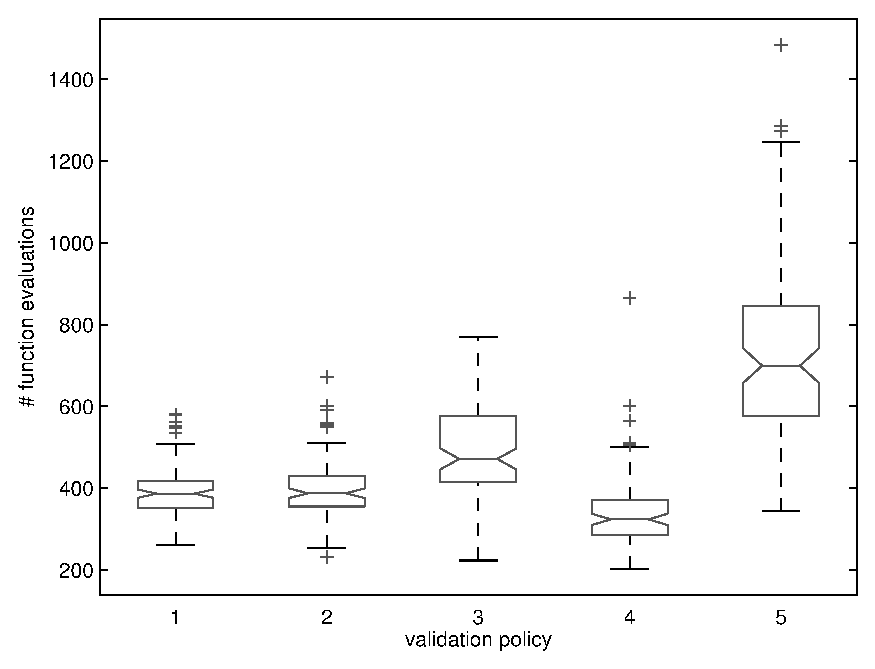
\includegraphics[width=\textwidth]{anova}
\caption[Box plot for different validation strategies]{Box plot for different validation methods~\cref{sur:val:org,sur:val:pseudo,sur:val:first,sur:val:last,sur:val:mubest} for Rosenbrock function of dimension $d=2$.}
\label{fig:boxplot}
\end{figure}

The surrogate ranking validation and improvement strategy using ordinal regression is tested using a Covariance Matrix Adaptation Evolution Strategy (CMA-ES) developed by \cite{Hansen01}. CMA-ES is a very efficient numerical optimization technique, however we still expect to reduce the number of function evaluations needed for search. For \cite{Ru06:PPSN} the validation policy had to successfully rank all of the candidate individuals, i.e.,  until $\tau=1$. %<viðbót vegna rýnis>
If there is no limit to training size then updating the surrogate becomes too computationally expensive, hence the training size needs to be pruned to size to $\overline{l}$. %</viðbót vegna rýnis>
\citeauthor{Ru06:PPSN} reduces the set to a size $\overline{l} = \lambda$ by omitting the oldest individuals first. These are quite stringent restrictions which can be improved upon. 
% Pruning away the worst - instead of the oldest 
The pruning only considers the age of the individuals, however older individuals might still be of more interest than newer ones if their fitness ranks higher. A more sophisticated way of pruning would be omitting the lowest ranking individuals first. 
% Validating on a mean pseudo individual  
Moreover, candidate individuals are generated randomly using a normal distribution, thus a pseudo individual representing their mean could be of interest as an indicator for the entire population, e.g., by validating this pseudo individual first could give information if the surrogate is outdated w.r.t. the current search space. 
% Validation only the current mu best ranked individuals 
Furthermore, the validation is only done on the candidate individuals for the current generation in ES where only the $\mu$ best ranked individuals will survive to become parents. In evolutionary computing one is interested in the accurate ranking of individuals  generated in the neighbourhood of parent individuals, hence for sufficient validation of the surrogate, only the $\mu$ best ranked individuals  should be considered and evaluated, since all other individuals  of lower rank will be disregarded in the next iteration in ES. 
% Validating on every other generation
Lastly, one should also investigate the frequency by which the model is validated, e.g., at each generation or every $K>1$ generations or even have the need for validating adapt with time.

Preliminary tests were conducted on which validation method deemed fruitful, by implementing  Rosenbrock function of dimension $d=2$, for the following setups, 
\begin{inparaenum}[{Method} (i)]
 \item the setup presented in \cite{Ru06:PPSN} %\label{sur:val:org}
 \item omitting the worst individuals during the pruning process, instead of the oldest ones; \label{sur:val:first}
 \item initialise the validation process by using a pseudo individual that represents the mean of the new candidate individuals; \label{sur:val:pseudo}
 \item requiring that only the $\mu$ best candidate individuals are correctly ranked; \label{sur:val:mubest}
\item validating on every other generation. \label{sur:val:last}
\end{inparaenum}
To summarise, the original method~\cref{sur:val:org} is compared with the aforementioned validation improvements, namely methods~\cref{sur:val:first,sur:val:pseudo,sur:val:mubest,sur:val:last}, which were added one at a time to the original method. 


Experimental results focusing on the number of true function evaluations are shown in~\cref{fig:boxplot}. There is no statistical difference between omitting oldest or worst ranked individuals  from the training set, but this was expected, since both are believed to be representatives of a region of the search space which is no longer of interest. Adding the pseudo mean candidate individual didn't increase the performance edge. When the surrogate was updated on every other generation, it quickly became outdated and more than double function evaluations were needed to achieve the same rate of convergence. 
However, requiring the correct ranking for only the $\mu$ best ranked candidate individuals showed a significant performance edge. 

If the training accuracy is not 100\% then clearly $\tau < 1$. In this case additional training individuals  would be forced for evaluation. However, enforcing a completely concordant ranking, i.e.,  $\tau=1$, was deemed to be too strict due to the fact the search is stochastic. Thus the surrogate is said to be sufficiently accurate if $\tau>0.999$. \todo{Af hverju 0.999? Rökstyðja betur}

Based on these preliminary tests, a pseudo code for the proposed model validation and improvement strategy is described in~\cref{fig:pseudocode} where it is implemented at the end of each generation of CMA-ES. The algorithm essentially only evaluates the expensive true fitness function when the surrogate is believed to have diverged. During each iteration of the validation process there are two sets of individuals, $\mathcal{Y}$ and $\mathcal{X}$, which are the training individuals  which have been evaluated with the expensive model, and the candidate individuals (of unknown fitness) for the next iteration of CMA-ES, respectively. The test individuals  of interest are those who are believed to become parent individuals  in the next generation of CMA-ES, i.e.,  the $\mu$ best ranked candidate individuals according to the surrogate $h$. The method uses only a simple cross-validation on a single test individual, the one which the surrogate ranks the highest and has not yet been added to the training set. Creating more test individuals  would be too costly, but plausible. Once a test individual has been evaluated it is added to the training set and the surrogate $h$ is updated w.r.t. $\mathcal{Y}$, cf.~\cref{fig:schema}. This is repeated until the surrogate is said to be sufficiently accurate, which occurs if either,
\begin{description}
  \item[$\tau$ sufficiently close], i.e.,  Kendall's $\tau$ statistic between the ranking of the training set using the surrogate, $\bar{R}$, and its true ranking, $R$, is higher than $0.999$, or 
  \item[$\mu$ best ranked] candidate individuals w.r.t. the current surrogate have been added to the training set.
\end{description}
Note that during each update of the surrogate of the ranking of the $\mu$ best candidate individuals can change. Thus it is possible to evaluate more then $\mu$ test individuals  during each validation iteration. 

Once the validation algorithm has completed, the training set is pruned to a size $\bar{l}=\lambda$ by omitting the lowest ranking individuals . \todo{Af hverju þetta gildi á $\bar{l}$?}

\begin{figure}
\noindent{\footnotesize\begin{tabbing}
\quad \quad \= 0\;\; \= \emph{Initialization}: Let $\mathcal{Y}$ denote current training set and its \\
\>   \> corresponding surrogate by $h$. Let $\mathcal{X}$ denote population \\
\>   \> of $\lambda$ individuals of unknown fitness under inspection.\\
\>1  \> {\bf for} \= $t := 1$ to $\lambda$ {\bf do} \emph{(validate a test individual )}\\ 
\>2  \>\> Estimate ranking of $\mathcal{X}$ using $h$; denoted by $\bar{R}_0$. \\
\>3  \>\> $\vec{x}_B \leftarrow \max_{\vec{x}\in\mathcal{X}\setminus\mathcal{Y}}\left\{\bar{R}_0\right\}$ (\emph{test individual}). \\
\>4  \>\> Rank $\vec{x}_B$ w.r.t. individuals  in $\mathcal{Y}$ using $h$; denoted by $\bar{R}$. \\
\>5  \>\> Evaluate $\vec{x}_B$ using true fitness function and evaluate its\\
\>   \>\> true rank among individuals  in $\mathcal{Y}$; denoted by $R$. \\ 
% In the case where no explicit fitness function can be defined, the test individual is evaluated by comparing it with selected individuals  in the training set.
\>6  \>\> $\mathcal{Y}\leftarrow\mathcal{Y}\cup\{\vec{x}_B\}$ \emph{(add to training set)}. \\
\>7  \>\> Compare the rankings  $\bar{R}$ and $R$ by computing the rank \\
\>   \>\> correlation $\tau$.\\
\>8  \>\> {\bf if} \= $\tau>0.999$ {\bf then} \\
\>9  \>\> \> break (\emph{model is sufficiently accurate}) \\
\>10 \>\> {\bf fi} \\
%This is a simple cross-validation on a single test individual. Creating more test individuals  would be too costly, but plausible.
\>11  \>\> Update the surrogate $h$ using the new training set $\mathcal{Y}$.\\
\>12  \>\> {\bf if} \= $\mu$ best individuals of $\bar{R}_0$ have been evaluated {\bf then} \\
\>13  \>\> \> break (\emph{model is sufficiently accurate}). \\
\>14  \>\> {\bf fi} \\
\>15  \> {\bf od} %  Repeated the steps 1-9 above until $\tau_t>0.999$ or at least the $\mu$  highest ranking individuals  of unknown fitness have been evaluated. There is no need to evaluate more than the $\mu$ best ranking individuals  since they will be disregarded in the next iteration of CMA-ES.
\end{tabbing}}
\caption{Pseudo code}
\label{fig:schema:pseudocode}
\end{figure}

\begin{figure} \centering 
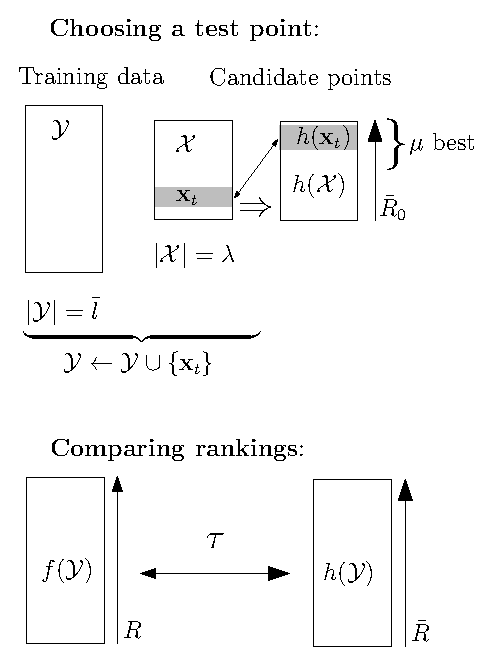
\includegraphics[width=0.5\textwidth]{schema}
\caption{Schema for validating and improving surrogate models.}\label{fig:schema} 
\end{figure}


\section{Experimental Study}\label{sec:sur:expr}
In the experimental study CMA-ES  is run for several test functions, namely sphere model and Rosenbrock function (cf.~\cref{app:fun:sphere} and~\cref{app:fun:rosen}), of various dimensions $d=2,5,10$ and $20$. The average fitness for $100$ independent runs versus the number of function evaluations is reported using the original validation procedure presented in \cite{Ru06:PPSN} and compared with its new and improved validation procedure, whose pseudo code is presented in~\cref{fig:schema:pseudocode} and shown schematically in~\cref{fig:schema}. The procedures will be referred to as using ``all'' or only the ``$\mu$ best'' candidate individuals during the validation, respectively.
The parameter setting for the $(\mu,\lambda)$ CMA-ES is as recommended in \cite{Hansen01} with population size $\lambda = 4+\lfloor 3\ln(n)\rfloor$ and the number of parents selected $\mu=\lambda/4$. The stopping criteria used are $1000n$ function evaluation or a fitness less than $10^{-10}$. The initial mean search individual is generated from a uniform distribution between $0$ and $1$. It is also noted that the training set is only pruned to size $\overline{l} = \lambda$ subsequent to the validation and improvement procedure.

\subsection{Sphere model}\label{sec:sphere}
The first experimental results are presented for the unimodal sphere model of dimension $d$.  
The average fitness versus the number of function evaluations is presented in~\cref{fig:sphereFitness}. A performance edge is achieved by restricting the validation strategy to only having the surrogate correctly rank the $\mu$ highest ranking individuals, and thereby saving the algorithm of evaluating individuals  that would have been disregarded in the next iteration.~\cref{fig:sphereIntmEval} shows the mean intermediate function evaluations that are calculated during the validation process. As one expects, requiring the method to evaluate no more than the $\mu$ best ranked candidate individuals results in a lower intermediate function evaluations, generally saving the method one function evaluation per generation, it also achieves a better mean fitness, as shown in~\cref{tbl:Sphere}.

\begin{figure}
%\subfloat[Mean fitness values versus number of function evaluation]{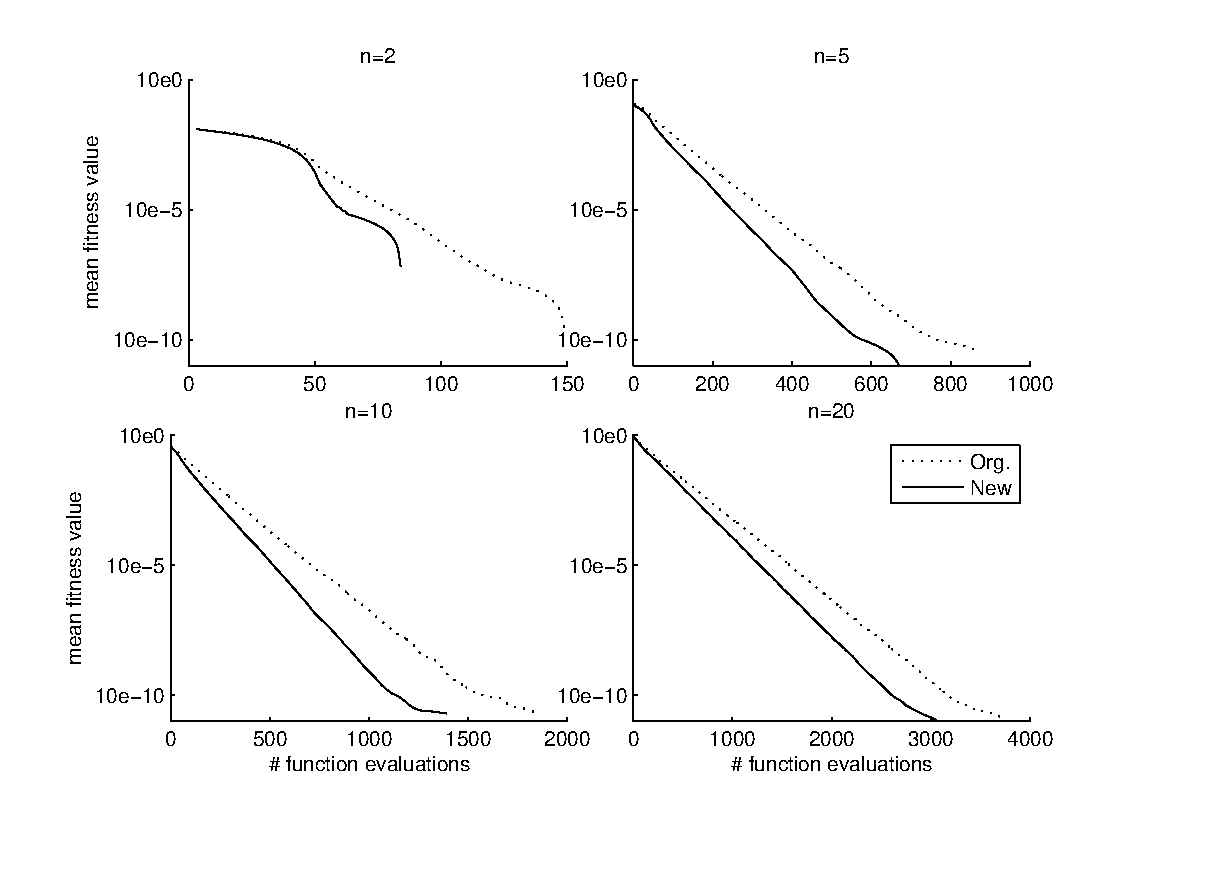
\includegraphics[trim = 8mm 10mm 10mm 5mm, clip, width=\textwidth]{sphere_meanFitness_funcEval}}
\label{fig:sphereFitness}
\,
%\subfloat[Mean intermediate function evaluations versus generation]{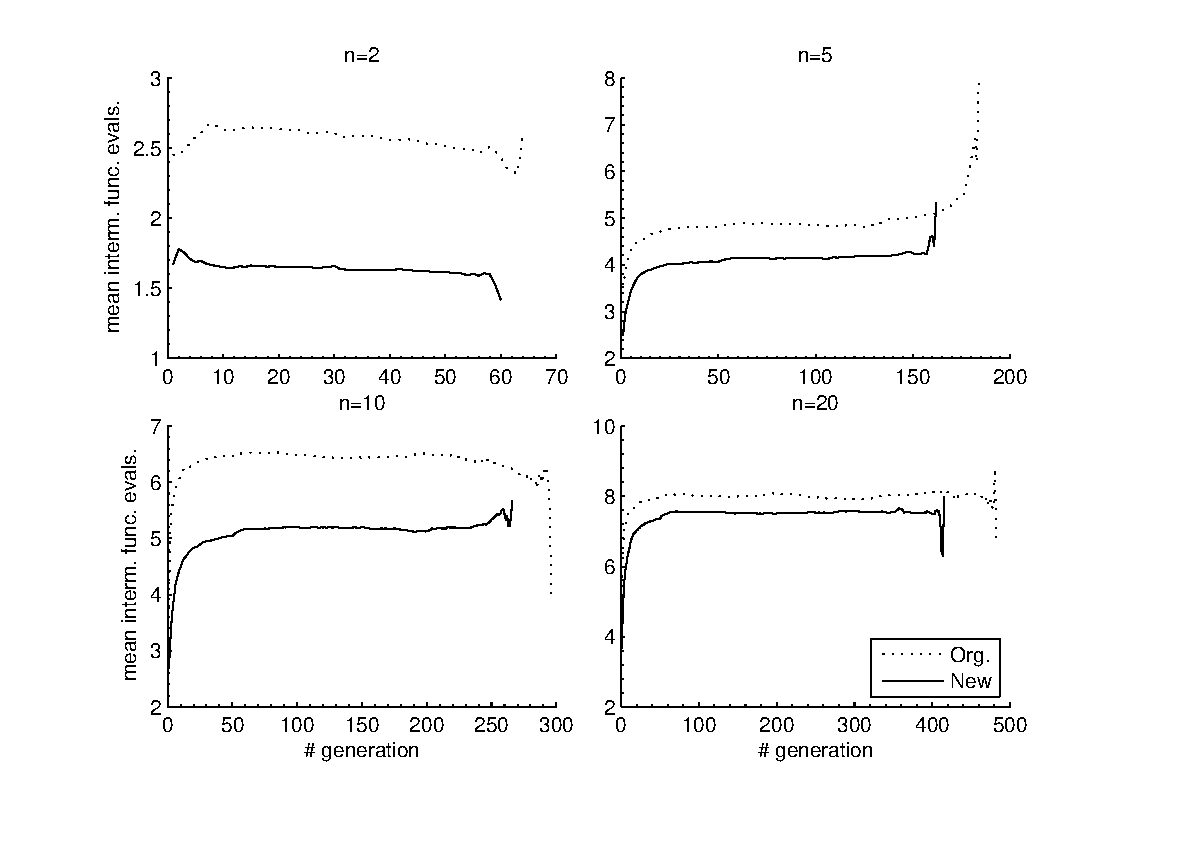
\includegraphics[trim = 10mm 10mm 10mm 5mm, clip, width=\textwidth]{sphere_intmEvals_gen}}
\label{fig:sphereIntmEval}
\caption{Sphere model: Surrogate updated using all (dotted) or $\mu$ best (solid) individuals.}
\end{figure}

\begin{table} \centering
\caption{Main statistics of experimental results for updating surrogate with all or $\mu$ best individuals on sphere model.}\label{tbl:Sphere}
{\renewcommand{\arraystretch}{1.1} \renewcommand{\tabcolsep}{0.1cm} %\scriptsize%footnotesize
\begin{tabular}{ c  c | rrr | rrr| rrr }
\toprule
 & & \multicolumn{3}{c|}{Function eval.} & \multicolumn{3}{c|}{Generations} & \multicolumn{3}{c}{Fitness} \\ 
     & $n$ & \multicolumn{1}{c}{mean} & \multicolumn{1}{c}{med.} & \multicolumn{1}{c|}{sd} & \multicolumn{1}{c}{mean} & \multicolumn{1}{c}{med.} & \multicolumn{1}{c|}{sd} & \multicolumn{1}{c}{mean} & \multicolumn{1}{c}{med.} & \multicolumn{1}{c}{sd} \\
\midrule
all& 2 & 130.59 & 132 & 18.33 & 49.02 & 49 & 6.51 & 2.35e-09 & 2.82e-10 & 1.15e-08\\ 
$\mu$&2 & 81.53 & 81 & 9.53 & 48.11 & 48 & 5.02 & 7.01e-10 & 2.26e-10 & 1.35e-09\\ \midrule
all& 5 & 702.02 & 702 & 67.57 & 145.15 & 145 & 14.96 & 2.77e-10 & 1.82e-10 & 3.64e-10\\ 
$\mu$& 5 & 545.25 & 547 & 54.27 & 132.60 & 132 & 11.03 & 1.83e-10 & 1.46e-10 & 1.09e-10\\ \midrule
all& 10 & 1563.58 & 1553 & 117.09 & 241.83 & 240 & 18.47 & 1.52e-10 & 1.37e-10 & 5.03e-11\\ 
$\mu$& 10 & 1161.03 & 1158 & 79.98 & 226.60 & 224 & 13.86 & 1.34e-10 & 1.22e-10 & 3.80e-11\\ \midrule
all& 20 & 3383.83 & 3377 & 135.52 & 423.14 & 424 & 20.42 & 1.27e-10 & 1.21e-10 & 2.51e-11\\ 
$\mu$& 20 & 2795.28 & 2804 & 132.77 & 372.86 & 372 & 16.56 & 1.17e-10 & 1.12e-10 & 1.72e-11\\ 
\bottomrule
\end{tabular}
}
\end{table}

\subsection{Rosenbrock function}\label{sec:rosen}
The first experiment is now repeated for Rosenbrock function.
The average fitness versus the number of function evaluations is presented in~\cref{fig:rosenFitness} and~\cref{fig:rosenIntmEval} shows the mean intermediate function evaluations that are calculated during the validation process. Despite requiring more generations, the over all function evaluations are significantly lower and yield a better fitness when updating the surrogate on only the $\mu$ best individuals as shown in~\cref{tbl:Rosenbrock}. If all of the candidate individuals have to be ranked correctly, the method will get stuck in local minima for this problem in around 6 out of 100 experiments, however this is not a problem if only the $\mu$ best candidate individuals are ranked consistently, except at high dimensions, and even then the $\mu$ best individuals  policy significantly outperforms evaluating all of the candidate individuals. Clearly the choice of validation policy will influence search performance. 

\begin{figure}
%\subfloat[Mean fitness values versus number of function evaluation]{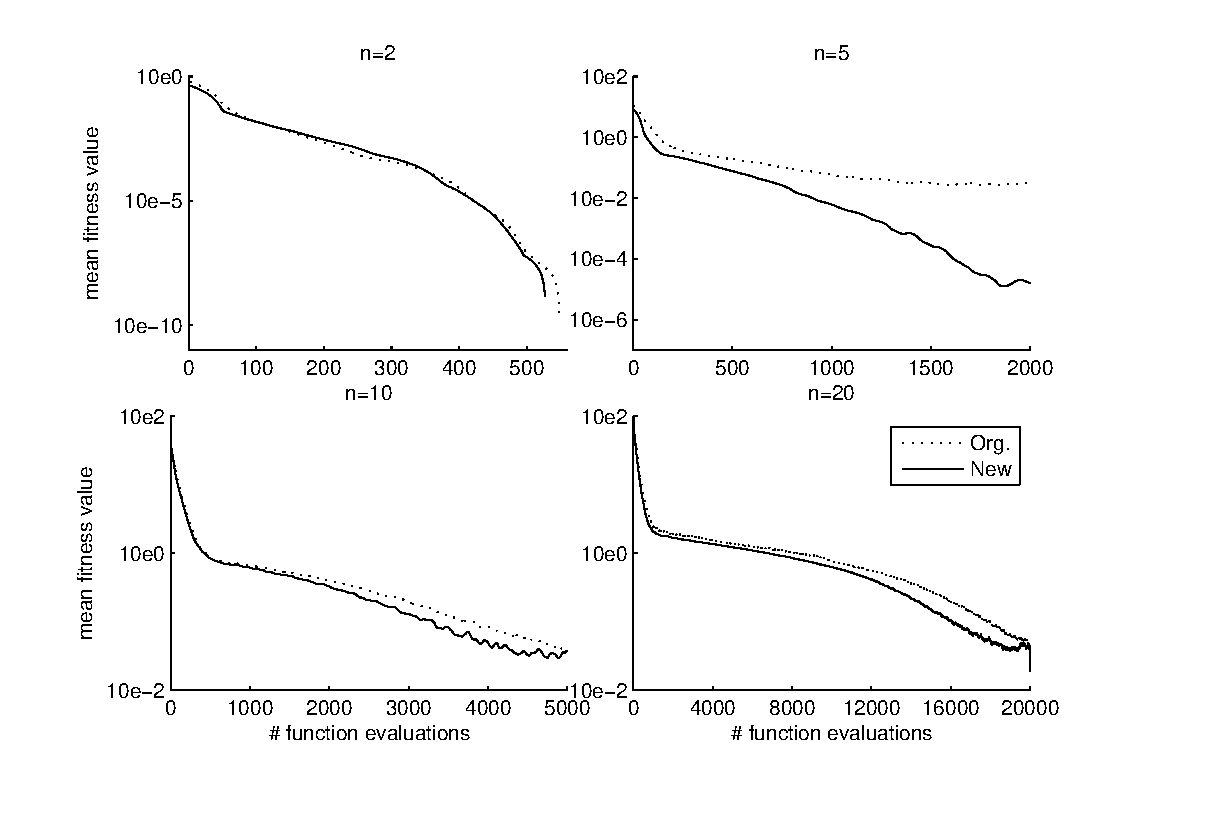
\includegraphics[trim = 10mm 10mm 10mm 5mm, clip, width=\textwidth]{rosen_meanFitness_funcEval}}
\label{fig:rosenFitness}
\,
%\subfloat[Mean intermediate function evaluations versus generation]{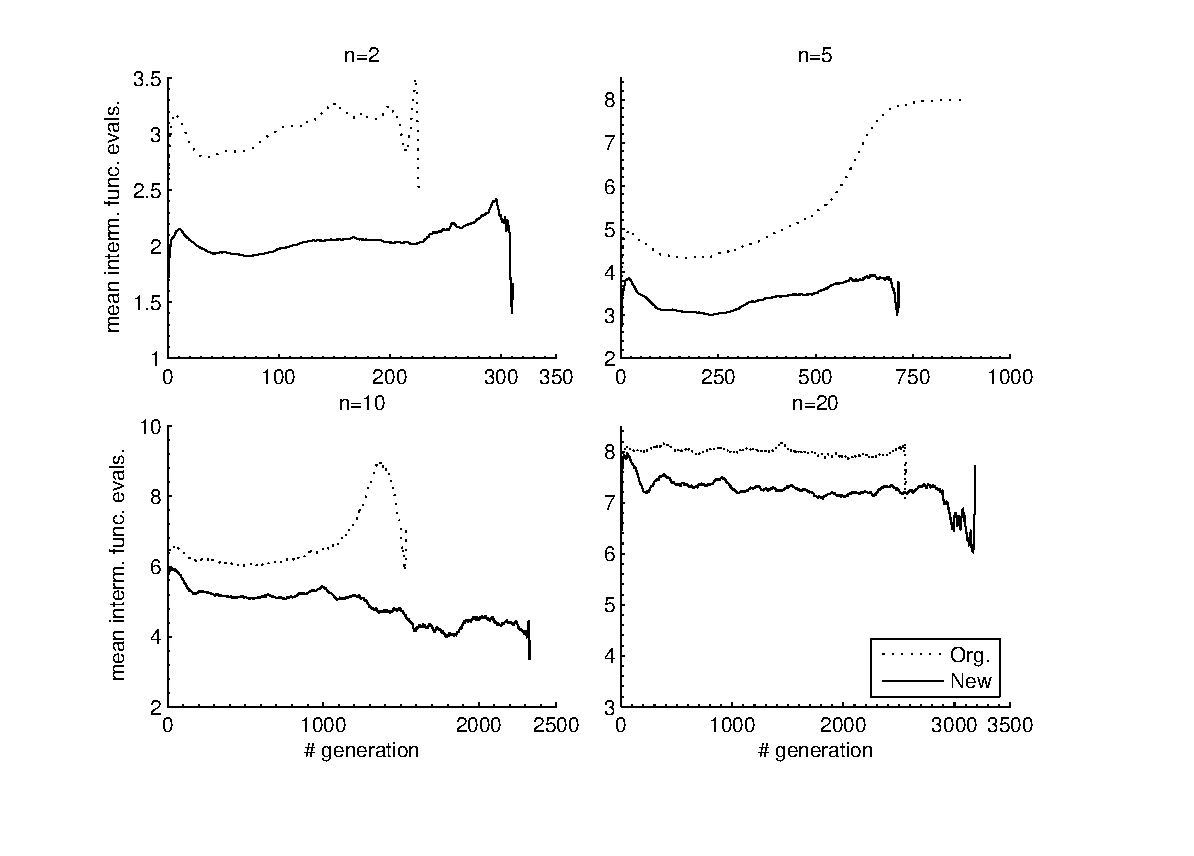
\includegraphics[trim = 15mm 10mm 15mm 5mm, clip, width=\textwidth]{rosen_intmEvals_gen}}
\label{fig:rosenIntmEval}
\caption{Rosenbrock function: Surrogate updated using all (dotted) or $\mu$ best (solid) individuals.}
\end{figure}

\begin{table}\centering
\caption{Main statistics of experimental results for updating surrogate with all or $\mu$ best individuals on Rosenbrock function.} \label{tbl:Rosenbrock}
{\renewcommand{\arraystretch}{1.1} \renewcommand{\tabcolsep}{0.1cm} %\scriptsize%footnotesize
\begin{tabular}{ c  c | rrr | rrr| rrr}
\toprule
 & & \multicolumn{3}{c|}{Function eval.} & \multicolumn{3}{c|}{Generations} & \multicolumn{3}{c}{Fitness} \\ 
     & $n$ & \multicolumn{1}{c}{mean} & \multicolumn{1}{c}{med.} & \multicolumn{1}{c|}{sd} & \multicolumn{1}{c}{mean} & \multicolumn{1}{c}{med.} & \multicolumn{1}{c|}{sd} & \multicolumn{1}{c}{mean} & \multicolumn{1}{c}{med.} & \multicolumn{1}{c}{sd} \\
\midrule
all & 2 & 389.9 & 386 & 63.9 & 132.3 & 130 & 31.3 & 6.24e-10 & 3.20e-10 & 1.05e-09\\ 
$\mu$ & 2 & 344.9 & 336 & 78.6 & 172.2 & 170 & 50.0 & 7.53e-10 & 1.66e-10 & 3.64e-09\\ \midrule
all & 5 & 2464.2 & 2280 & 748.6 & 514.6 & 492 & 105.8 & 2.75e-01 & 1.74e-10 & 1.01e+00\\ 
$\mu$ & 5 & 1724.9 & 1729 & 295.6 & 520.7 & 520 & 82.8 & 1.83e-10 & 1.53e-10 & 1.05e-10\\ \midrule
all & 10 & 6800.5 & 6495 & 1258.7 & 1079.8 & 1052 & 177.8 & 2.79e-01 & 1.32e-10 & 1.02e+00\\ 
$\mu$ & 10 & 6138.5 & 6143 & 1398.2 & 1177.7 & 1103 & 310.1 & 1.99e-01 & 1.24e-10 & 8.73e-01\\ \midrule
all & 20 & 19968.8 & 20004 & 234.7 & 2494.0 & 2500 & 49.6 & 4.54e-01 & 2.88e-02 & 1.08e+00\\ 
$\mu$ & 20 & 19645.9 & 20002 & 1086.4 & 2687.3 & 2748 & 230.5 & 3.10e-01 & 3.12e-07 & 9.97e-01\\ \bottomrule
\end{tabular}
}

\end{table}

\section{Discussion and Conclusion}\label{sec:sur:disc}
The technique presented in this dissertation to control the number of true fitness evaluations is based on a single test individual chosen from a set of candidate individuals which the surrogate ranks the highest. The approximate ranking of this test individual is compared with its true ranking in order to determine the quality of the surrogate. This is a simple form of cross-validation. An alternative approach could be to rank all candidate individuals along with the training individuals  using the surrogate model. This is followed by the re-ranking of training and candidate individuals using the updated surrogate and comparing it with the previous estimate by computing Kendall's $\tau$. Its aim is to observe a change in ranking between successive updates of the surrogate. This study has shown that during the validation process it is sufficient for $\tau$ to be close to $1$ or that only the potential parent individuals should be ranked consistently. \todo{Report \% close to 1 vs. only $\mu$ best}.\\
Moreover, the new validation approach reduces the number of fitness evaluation needed, without a loss in performance although it might take a few more iterations in CMA-ES. 


When it comes to modelling surrogates based on training data, the general rule of thumb is the bigger the training set, the more accurate a model. However, there are computational time limits thus pruning of the training set is necessary. Previous studies \citep{Jin05,Ratle99} have reported that replacing random training individuals  is not optimal. This study has shown that there is no statistical difference in omitting oldest or lowest-ranking individuals  from the training set. Hence, for future work, further investigation on the fitness landscape is needed to determine effectively which search area is no longer of interest and thus unnecessary for the surrogate to approximate correctly. For instance it could be of interest to disregard training individuals  with the largest euclidean distance away from the current candidate individuals rather than simply omitting the oldest/lowest-ranking training individuals. 

When building surrogates in evolutionary computation one is interested in the quality of ranking of individuals  rather than their exact fitness value. For this reason the training accuracy and cross validation is a more meaningful measure of quality for the surrogate model. This is in contrast to regression, where the fitness function is modelled directly and the quality estimated in terms of measures such a least square error. 
This study has shown that the sampling used for validating the accuracy of the surrogate can stop once the $\mu$ best ranked candidate individuals have been evaluated, since they are the only candidate individuals who will survive to become parents in the next generation. 
Although in some cases the sampling could stop sooner, when the surrogate ranking and true ranking are sufficiently concordant, i.e.,  $\tau$ was close to 1. This slight slack in for $\tau$ is allowed due to the fact the ES search is stochastic, however the allowable range in slack for $\tau$ needs to be investigated more fully % <viðbót vegna rýnis>
since allowing only $\tau\in[0.999,1]$ might be too narrow an interval, resulting in an excess of expensive function evaluations needed. %</viðbót vegna rýnis>

However, in the context of surrogate-assisted optimization the discrepancy between the exact model and its surrogate can be translated as noise, which could be an indicator of the necessary sampling size for validation/updating the surrogate, instead of only focusing on consistently ranking the $\mu$ best candidate individuals. Therefore, one can take inspiration from a varying random walk population model suggested by \cite{Miller97} to approximate the population sizing to overcome unnecessary fitness evaluations.
  
  
  \ifthenelse{\equal{#1}{true}}{
%    \HeaderQuote{What is the use of a book, without pictures or conversations?}{Alice}

\chapter{Test function suite}\label{app:fun} \todo[color=green!40]{\cref{app:fun} Unfinished}
\FirstSentence{T}{est functions $f$ used} in~\cref{ch:surrogates} are defined $f:\mathbb{R}^d\mapsto\mathbb{R}$.

\todo[inline]{All benchmark functions with the exception of ?? are described in [?]. They are summarized here for completeness. The original sources of the functions are also cited.
	\url{https://notendur.hi.is/tpr/software/sres/testfcn.pdf}
}

\section{Sphere }\label{app:fun:sphere}
Sphere function is a convex and unimodal function (cf.~\cref{fig:fun:sphere}). Sphere function is defined as follows,
\begin{eqnarray}
	f_{\textrm{Sphere}}(\vec{x})&=&\sum_{i=1}^d x_i^2
\end{eqnarray} where $\vec{x}\in[-3,7]^d$.
It has a global minimum at $\vec{x}=\textbf{0}$ where $f_{\textrm{Sphere}}(\textbf{0})=0$. 

\section{Noisy sphere}\label{app:fun:nsphere}
Noisy sphere function is the sphere function from~\cref{app:fun:sphere} where a Gaussian noise has added to perturb the sphere (cf.~\cref{fig:fun:nsphere} where $\epsilon=0.1$). Noisy sphere function is defined as follows,
\begin{eqnarray}
	f_{\textrm{NoisySphere}}(\vec{x})&=&f_{\textrm{Sphere}}(\vec{x})\left(1+\epsilon\mathcal{N}(0,1)\right)
\end{eqnarray} where $\vec{x}\in[-3,7]^d$.
It has a global minimum at $\vec{x}=\textbf{0}$ where $f_{\textrm{NoisySphere}}(\textbf{0})=0$.

\section{Schwefel}\label{app:fun:schwefel}
Schwefel is ... (cf.~\cref{fig:fun:schwefel}). Schwefel function is defined as follows,
\begin{eqnarray}
	f_{\textrm{Schwefel}}(\vec{x})&=&\sum_{i=1}^d\left(\sum_{j=1}^i x_j\right)^2
\end{eqnarray} where $\vec{x}\in[-10,10]^d$.
It has a global minimum at $\vec{x}=\textbf{0}$ where $f_{\textrm{Schwefel}}(\textbf{0})=0$.

\section{Ellipsoid}\label{app:fun:ellipsoid}
Ellipsoid is ... (cf.~\cref{fig:fun:ellipsoid}). Ellipsoid function is defined as follows,
\begin{eqnarray}f_{\textrm{Ellipsoid}}(\vec{x})=\sum_{i=1}^d \left(100^{\frac{i-1}{d-1}}x_i\right)^2
\end{eqnarray} where $\vec{x}\in[-3,7]^d$.
It has a global minimum at $\vec{x}=\textbf{0}$ where $f_{\textrm{Ellipsoid}}(\textbf{0})=0$.

\section{Rosenbrock}\label{app:fun:rosen}
Rosenbrock function is a non-convex function, where the global minimum is inside a long, narrow, parabolic shaped flat valley (cf.~\cref{fig:fun:rosen}). To find the valley is trivial. To converge to the global minimum, however, is difficult. Rosenbrock function is defined as follows,
\begin{eqnarray}
	f_{\textrm{Rosenbrock}}(\vec{x})&=&\sum_{i=1}^{d-1} \left(100\cdot(x_i^2-x_{i+1})^2+(x_i-1)^2\right)
\end{eqnarray} where $\vec{x}\in[-5,5]^d$. 
It has a global minimum at $\vec{x}=\textbf{1}$ where $f_{\textrm{Rosenbrock}}(\textbf{1})=0$.

\section{Ackley}\label{app:fun:ackley}
Ackley function is a non-convex function, where the function is a fairly difficult problem due to its large search space and its large number of local minima (cf.~\cref{fig:fun:ackley}). Ackley function is defined as follows,
\begin{eqnarray}
	f_{\textrm{Ackley}}(\vec{x})&=&20-20\cdot\exp\left(-0.2\sqrt{\frac{1}{n}\sum_{i=1}^d x_i^2}\right)
	\\&&+e-\exp\left(\frac{1}{2}\sum_{i=1}^d \cos(2\pi x_i)\right) \nonumber
\end{eqnarray} where $\vec{x}\in[1,30]^d$.
It has a global minimum at $\vec{x}=\textbf{0}$ where $f_{\textrm{Ackley}}(\textbf{0})=0$.

\section{Rastrigin}\label{app:fun:rastrigin}
Rastrigin function is based on the sphere function from~\cref{app:fun:sphere} with the addition of cosine modulation in order to produce frequent local minima (cf.~\cref{fig:fun:rastrigin}). Thus, the test function is highly multimodal. However, the location of the minima are regularly distributed. Rastrigin function is defined as follows,
\begin{eqnarray}
	f_{\textrm{Rastrigin}}(\vec{x})&=&10n+\sum_{i=1}^d \left(x_i^2-10\cos(2\pi x_i)\right)
\end{eqnarray} where $\vec{x}\in[1,5]^d$. 
It has a global minimum at $\vec{x}=\textbf{0}$ where $f_{\textrm{Rastrigin}}(\textbf{0})=0$.

\begin{figure}\centering
	\begin{subfigure}{0.37\textwidth}
		\centering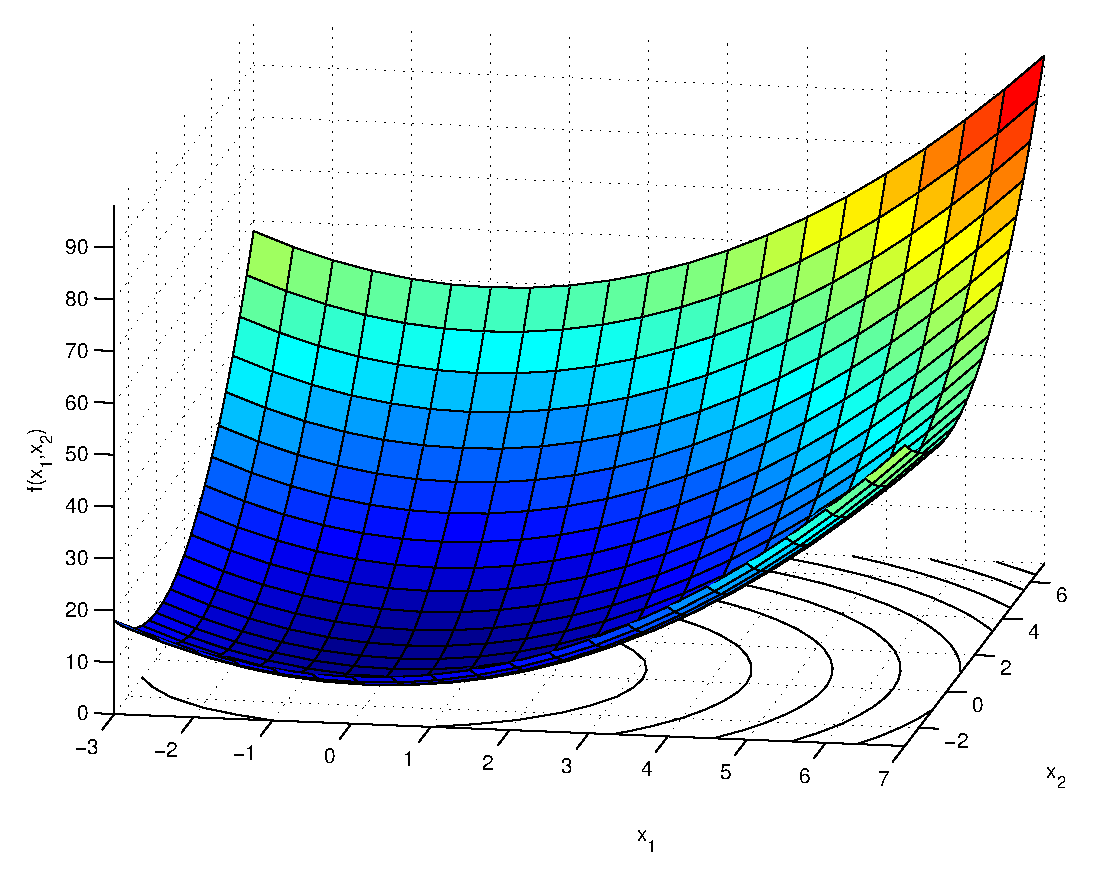
\includegraphics{fun/sphere}
		\caption{Sphere function}\label{fig:fun:sphere}
	\end{subfigure}
	\quad
	\begin{subfigure}{0.37\textwidth}
		\centering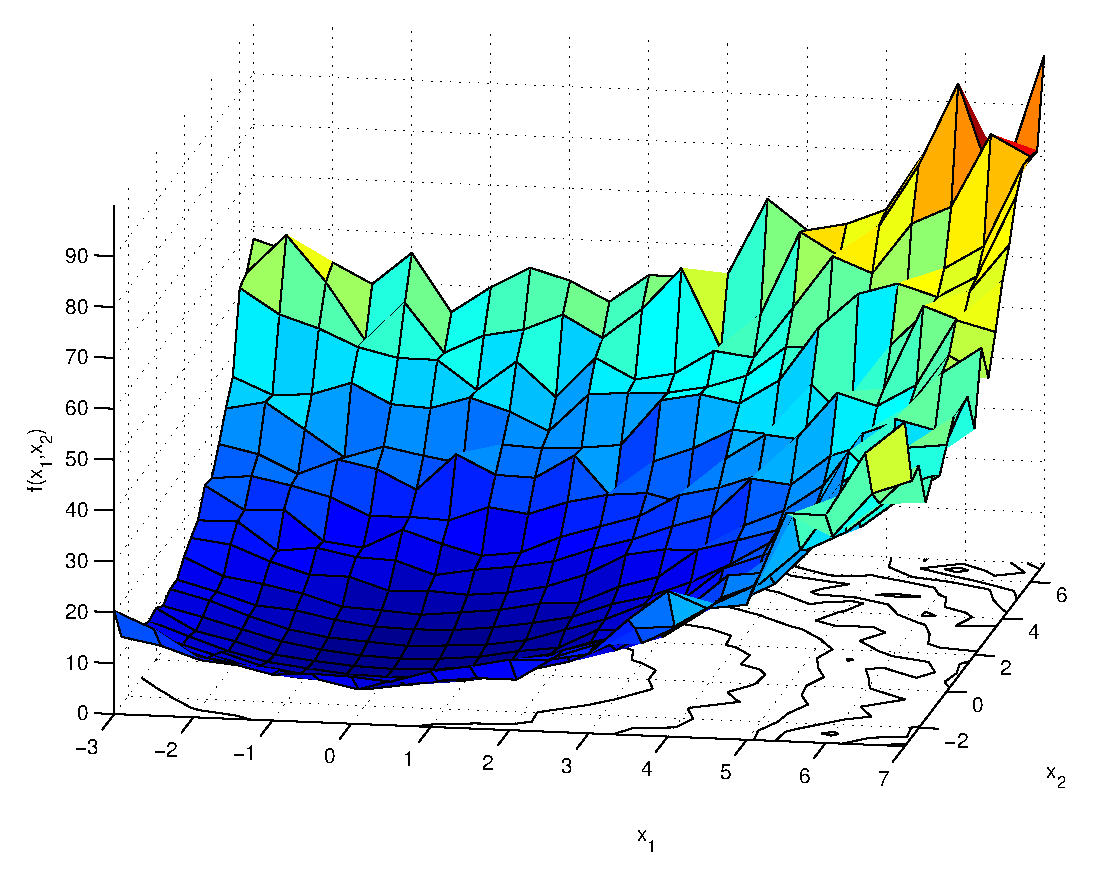
\includegraphics{fun/nsphere}
		\caption{Noisy sphere (with $\epsilon=0.1$)}\label{fig:fun:nsphere}
	\end{subfigure}
	\\
	\begin{subfigure}{0.37\textwidth}
		\centering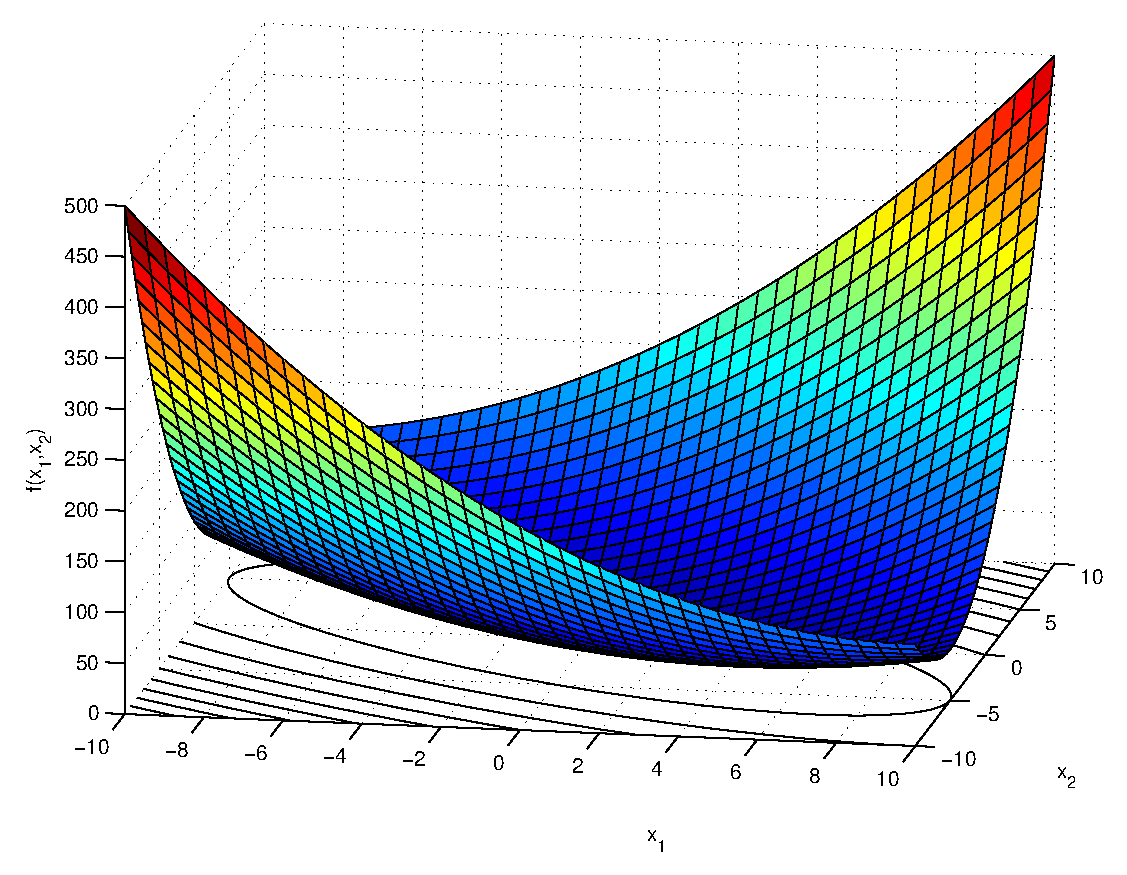
\includegraphics{fun/schwefel}
		\caption{Schwefel}\label{fig:fun:schwefel}
	\end{subfigure}
	\quad
	\begin{subfigure}{0.37\textwidth}
		\centering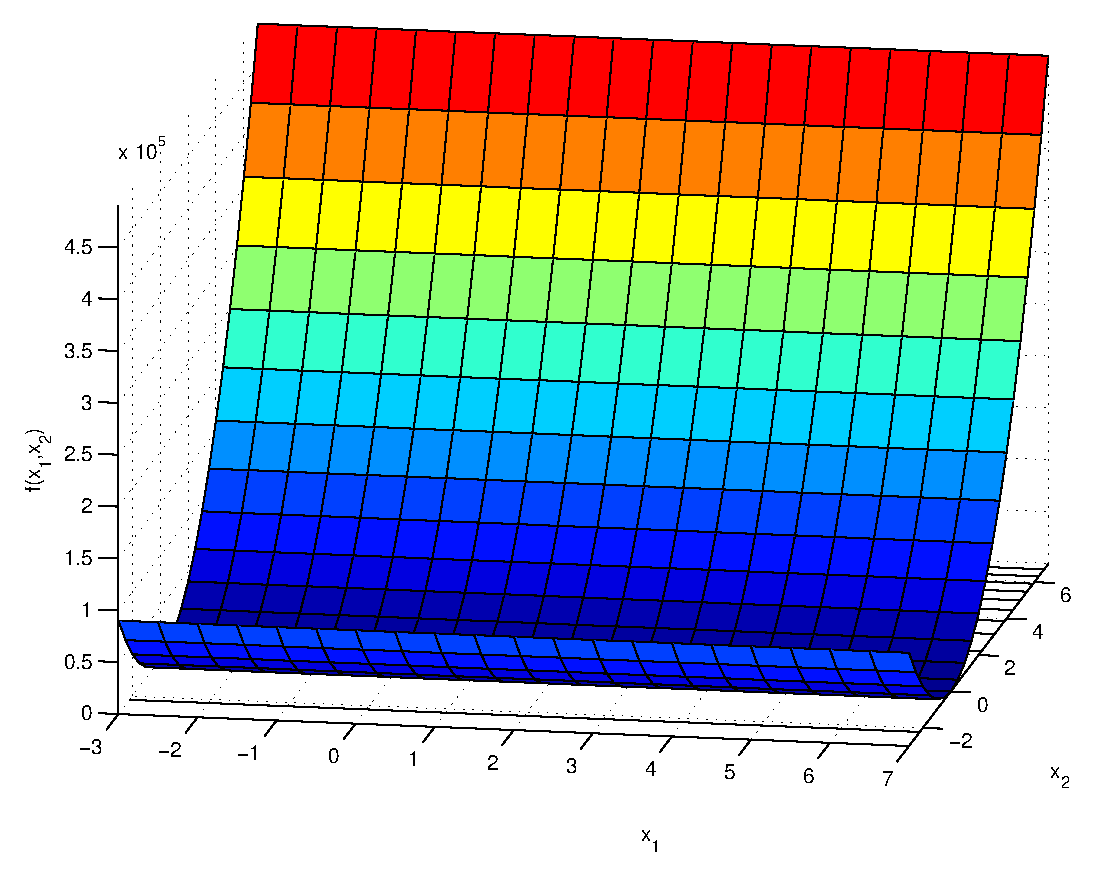
\includegraphics{fun/ellipsoid}
		\caption{Ellipsoid}\label{fig:fun:ellipsoid}
	\end{subfigure}
	\\
	\begin{subfigure}{0.37\textwidth}
		\centering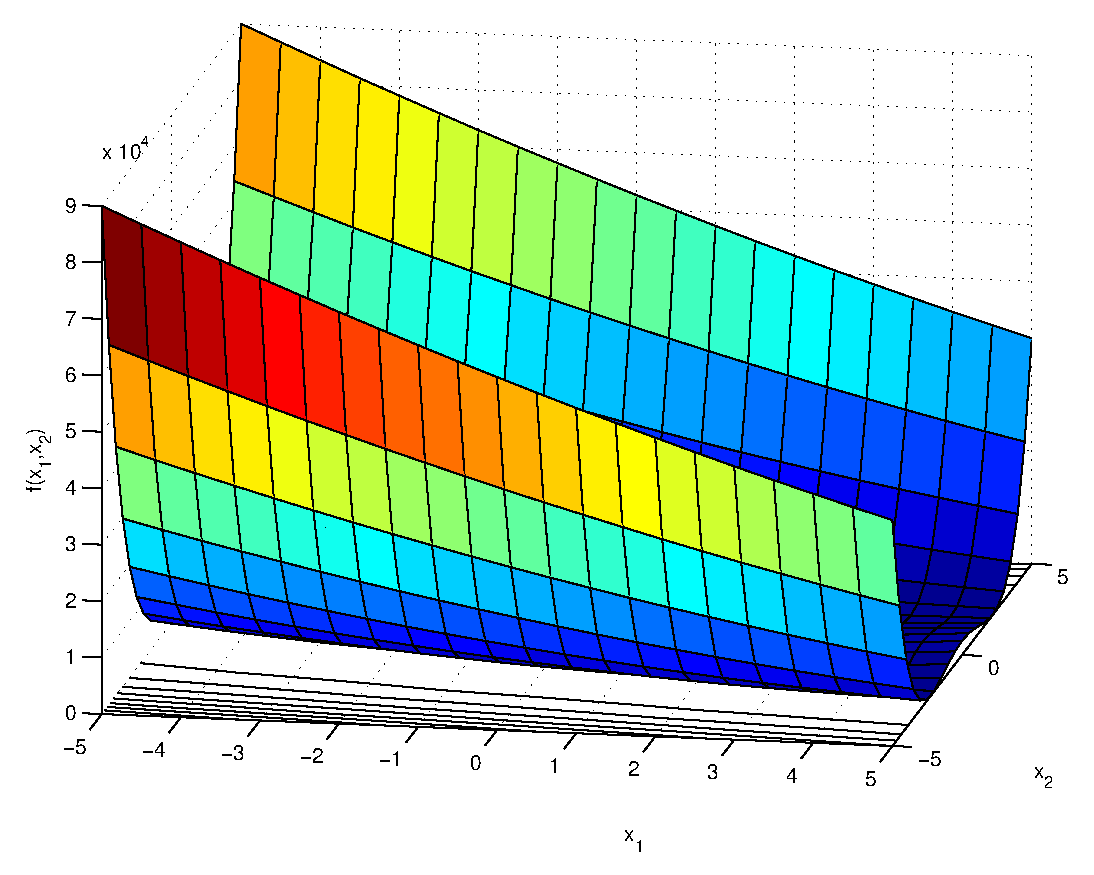
\includegraphics{fun/rosen}
		\caption{Rosenbrock}\label{fig:fun:rosen}
	\end{subfigure}
	\quad
	\begin{subfigure}{0.37\textwidth}
		\centering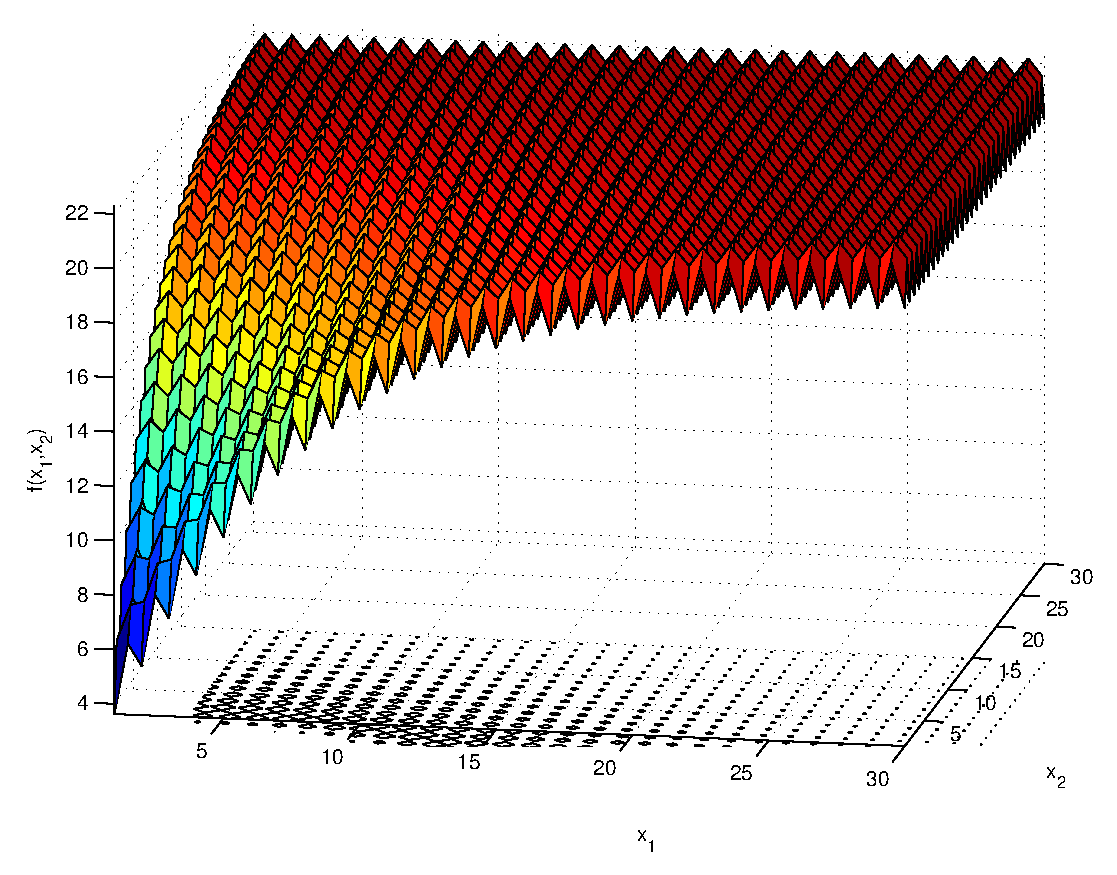
\includegraphics{fun/ackley}
		\caption{Ackley}\label{fig:fun:ackley}
	\end{subfigure}
	\\
	\begin{subfigure}{0.37\textwidth}
		\centering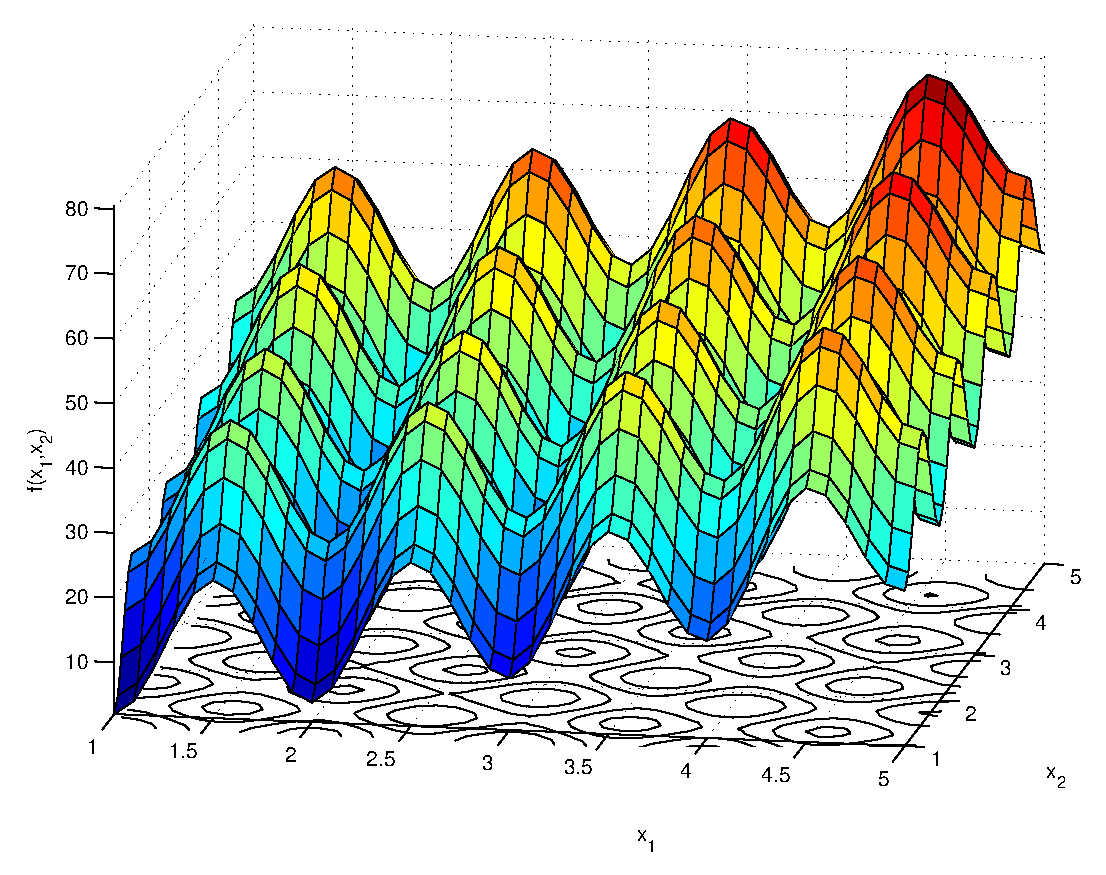
\includegraphics{fun/rastrigin}
		\caption{Rastrigin}\label{fig:fun:rastrigin}
	\end{subfigure}
	\caption{Test function suite of two variables in 3D.}
\end{figure}





 % test function suite
    \papers

\HeaderQuote{But it's no use going back to yesterday, because I was a different 
person then.}{Alice}
\chapter{\usebibentry{InRu11a}{title}}\label[paper]{InRu11a}
\paper{natbib=InRu11a,file={papers/InRu11a.pdf},
    authorslist={Helga Ingimundardóttir, Tómas Philip Rúnarsson}}

\chapter{\usebibentry{InRu11b}{title}}\label[paper]{InRu11b}
\paper{natbib=InRu11b,file={papers/InRu11b.pdf},
    authorslist={Helga Ingimundardóttir, Tómas Philip Rúnarsson}}

\chapter{\usebibentry{InRu12}{title}}\label[paper]{InRu12}
\paper{natbib=InRu12,file={papers/InRu12.pdf},
    authorslist={Helga Ingimundardóttir, Tómas Philip Rúnarsson}}

\chapter{\usebibentry{InRu14}{title}}\label[paper]{InRu14}
\paper{natbib=InRu14,file={papers/InRu14.pdf},
    authorslist={Helga Ingimundardóttir, Tómas Philip Rúnarsson}}

\chapter{\usebibentry{InRu15a}{title}}\label[paper]{InRu15a}
\paper{natbib=InRu15a,file={papers/InRu15a.pdf},
    authorslist={Helga Ingimundardóttir, Tómas Philip Rúnarsson},
    remark=Nominated for best paper}
 % published papers etc.
    \FirstSentence{T}{his thesis was typeset} using \LaTeX, originally developed by 
Leslie Lamport and based on Donald Knuth's \TeX. The body text is set in 11 
point Arno Pro, designed by Robert Slimbach in the style of book types from the 
Aldine Press in Venice, and issued by Adobe in 2007. A template, which can be 
used to format a Ph.D. thesis with this look and feel, has been released under 
the permissive creative commons share-alike license, and can be found on-line at
 \href{https://github.com/tungufoss/alice.papers/Thesis}{github.com/tungufoss/alice.papers}
or from the author at \href{mailto:hei2@hi.is}{hei2@hi.is}. 

Moreover the epigraphs are from \emph{Alice's Adventures in Wonderland} 
\citeyearpar{alice} and \emph{Through the Looking-Glass, and What Alice Found 
There} \citeyearpar{lookingglass} by Lewis \citeauthor{alice}.  
    }{}
  \ifthenelse{\equal{#1}{false}}{}{}
}
\newcommand{\printAll}{true} % either true or false CASE-SENSITIVE

\begin{document}

% Front matter
\printFrontMatter{\printAll}

% Main matter, include each chapter...
\include{chapters/introduction}
\HeaderQuote{Read the directions and directly you will be directed in the right direction.}{Doorknob} 

\chapter{Scheduling}\label{ch:scheduling}
\FirstSentence{S}{cheduling problems}, which occur frequently in practice, are a category within combinatorial optimisation problems. 
A subclass of scheduling problems is the \jsp\ scheduling problem (\JSP), which is widely studied in operations research. 
\Jsp\ deals with the allocation of tasks of competing resources where its goal is to optimise a single or multiple objectives. 
\Jsp's analogy is from manufacturing industry where a set of jobs are broken down into tasks that must be processed on several machines in a workshop. 
Furthermore, its formulation can be applied on a wide variety of practical problems in real-life applications which involve decision making, therefore its problem-solving capabilities has a high impact on many manufacturing organisation. % Gefa dæmi?

Deterministic \JSP\ is the most \emph{general} case for classical scheduling problems \citep{Jain99}. 
Many other scheduling problems can be reformulated as \JSP. 
For instance the widely studied \textit{Travelling Salesman Problem} can be contrived as \jsp\ with the salesman as a single machine in use and the cities to be visited are the jobs to be processed.
Moreover, the general form of \JSP\ assumes that each job can have its own distinctive flow pattern through the machines, which is independent of the other jobs. 
In the case where all jobs share the same permutation route, \jsp\ is reduced to a permutation \fsp\ scheduling problem (\FSP) \citep{Guinet1998,Tay08}. 
Therefore, without loss of generality, this dissertation is structured around \JSP. 

\section{\Jsp\ scheduling problem}
\JSP\ considered for this dissertation is where $n$ jobs, $\mathcal{J}=\{J_j\}_{j=1}^n$, are scheduled on a finite set, $\mathcal{M}=\{M_a\}_{a=1}^m$, of $m$ machines, subject to the constraint that each job $J_j$ must follow a predefined machine order (a chain or sequence of $m$ operations, $\vsigma_j=[\sigma_{j1},\sigma_{j2},\dotsc,\sigma_{jm}]$) and that a machine can handle at most one job at a time. 
The objective is to schedule jobs in such a manner as to minimise the maximum completion times for all tasks, which is also known as the makespan, $C_{\max}$. A common notion for this family of scheduling problems, i.e., a $m$ machine \JSP\ w.r.t. minimising makespan, is $Jm||C_{\max}$ \citep[cf.][]{Pinedo08}. In addition, for \FSP\ w.r.t. minimising makespan the notation is $Fm||C_{\max}$. 
An additional constraint commonly considered are job release-dates and due-dates, and then the objective is generally minimising the maximum lateness, denoted $Jm||L_{\max}$, however, those  constraints will not be considered here. 

Henceforth, the index $j$ refers to a job $J_j\in\mathcal{J}$ while the index $a$ refers to a machine $M_a\in\mathcal{M}$. If a job requires a number of processing steps or operations, then the pair $(j,a)$ refers to the operation, i.e., processing the task of job $J_j$ on machine $M_a$. Moreover, index $k$ will denote the time step of the operation. Note that once an operation is started, it must be completed uninterrupted, i.e., pre-emption is not allowed. Moreover, there are no sequence dependent setup times.

\section{Mathematical formulation}
For any given \JSP, which consists of $n$ jobs for $m$ machines, then each job $J_j$ has an indivisible operation time (or cost) on machine $M_a$, $p_{ja}$, which is assumed to be integral and finite. 
Starting time of job $J_j$ on machine $M_a$ is denoted $x_s(j,a)$ and its completion time is denoted $x_f(j,a)$ where, 
\begin{equation}  x_f(j,a):=x_s(j,a)+p_{ja} \end{equation} 
Each job $J_j$ has a specified processing order through the machines, it is a permutation vector, $\vsigma_j$, of $\{1,..,m\}$, representing a job $J_j$ can be processed on $M_{\vsigma_j(a)}$ only after it has been completely processed on $M_{\vsigma_j(a-1)}$, i.e.,
\begin{equation}\label{eq:permutation}
   x_s(j,\vsigma_j(a)) \geq x_f(j,\vsigma_j(a-1)) 
\end{equation}
for all $J_j\in\mathcal{J}$ and $a\in\{2,..,m\}$. 
Note, that each job can have its own distinctive flow pattern through the machines, which is independent of the other jobs. However, in the case that all jobs share the same permutation route, \JSP\ is reduced to a \FSP\ \citep{Guinet1998,Tay08}.

The disjunctive condition that each machine can handle at most one job at a time is the following,
\begin{equation}\label{eq:oneJobPerMac}
   x_s(j,a) \geq x_f(j',a) \quad\textrm{or}\quad x_s(j',a) \geq x_f(j,a)  
\end{equation}
for all $J_j,J_{j'}\in\mathcal{J},\; J_j\neq J_{j'}$ and $M_a\in\mathcal{M}$. 

The objective function is to minimise its maximum completion times for all tasks, commonly referred to as the makespan, $C_{\max}$, which is defined as follows,
\begin{equation}
  C_{\max} := \max\{x_f(j,\vsigma_j(m))\;|\;J_j\in\mathcal{J}\}.\label{eq:makespan}
\end{equation} 
Clearly, w.r.t. minimum makespan, it is preferred that schedules are non-delay, i.e., the machines are not kept idle. The time in which machine $M_a$ is idle between consecutive jobs $J_j$ and $J_{j'}$ is called idle time, or flow, 
\begin{equation} s(a,j):=x_s(j,a)-x_f(j',a) \label{eq:slack}\end{equation}
where $J_j$ is the immediate successor of $J_{j'}$ on $M_a$. Although this is not a variable directly needed to construct a schedule for \JSP, it is a key feature in order to measure the quality of the schedule. 

\section{Construction heuristics}\label{sec:CH}
Construction heuristics are designed in such a way that it limits the search space in a logical manner, respecting not to exclude the optimum. Here, the construction heuristic is to schedule the dispatches as closely together as possible, i.e., minimise the schedule's flow. 
More specifically, once an operation $(j,a)$ has been chosen from the ready-list, $\mathcal{R}$, by some dispatching rule, it can placed immediately after (but not prior) $x_f(j,\vsigma_j(a-1))$ on machine $M_a$ due to constraint \cref{eq:permutation}. 
However to guarantee that constraint \cref{eq:oneJobPerMac} is not violated, idle times $M_a$ are inspected, as they create flow time  which $J_j$ can occupy. Bearing in mind that $J_j$ release time is $x_f(j,\vsigma_j(a-1))$ one cannot implement \cref{eq:slack} directly, instead it has to be updated as follows,
\begin{eqnarray}
\tilde{s}(a,j')&:=& x_s(j'',a)-\max\{x_f(j',a),x_f(j,\vsigma_j(a-1))\} % \textrm{ if } x_f(j,\vsigma_j(a-1)\geq x_f(j',a) 
\end{eqnarray}
for all already dispatched jobs $J_{j'},J_{j''}\in \mathcal{J}_a$ where $J_{j''}$ is $J_{j'}$ successor on $M_a$. Since pre-emption is not allowed, the only applicable slots are whose idle time can process the entire operation, i.e.,
\begin{eqnarray}
\tilde{S}_{ja}&:=&\{J_{j'}\in \mathcal{J}_a\;|\;\tilde{s}(a,j')\geq p_{ja} \}\label{eq:slots}.
\end{eqnarray} 
Now, there are several heuristic methods for selecting a slot from \cref{eq:slots}, e.g., if the main concern were to utilise the slot space, then choosing the slot with the smallest idle time would yield a closer-fitted schedule and leaving greater idle times undiminished for subsequent dispatches on $M_a$. However dispatching $J_j$ in the first slot would result in its earliest possible release time, which would be beneficial for subsequent dispatches for $J_j$. Preliminary experiments favoured dispatching in the first (earliest) slot,\footnote{Preliminary experiments of 500 \JSP\ instances where inspected: First slot chosen could always achieve its known optimum by implementing the pseudo code in \cref{fig:pseudocode}, however only $97\%$ of the instances when choosing the smallest slot.} and henceforth will be used throughout the dissertation.

\begin{comment} % virðist að þetta vandamál sé leyst, sbr. "scriptCompareSlotChoice.m"
Preliminary experiments which at each time step all jobs on the ready-list are explored and dispatched according to a (fixed) construction heuristic. The job corresponding to the best resulting makespan (found via analytical methods) is chosen to have the highest priority. The resulting makespan is divided by its theoretical optimal makespan, i.e., the deviation from optimality defined by \cref{eq:ratio}. A histogram for 6-job 5-machine \jsp\ problem instances ($N=500$) is depicted in \cref{fig:slot:smallestvsfirst} using both the intrinsic heuristics: (\subref{fig:slot:first}) first slot chosen and (\subref{fig:slot:small}) slot corresponding to the smallest slot size chosen. Using always the first slot, roughly 26\% of the instances were able to achieve the optimum makespan, however mere 16\% using the smallest slot size. Hence dispatching in the first slot was favoured and will be used throughout the study.
\begin{figure}
\subfloat[First slot]{\includegraphics[width=\textwidth]{slotsize_first.eps}} %\label{fig:slot:first}}
\subfloat[Smallest slot size]{\includegraphics[width=\textwidth]{slotsize_small.eps}} %\label{fig:slot:small}}
\caption{Histogram of deviation from optimality by sequentially dispatching optimal jobs using a fixed construction heuristic.}
\label{fig:slot:smallestvsfirst}
\end{figure}
\end{comment}

Note that the choice of slot is an intrinsic heuristic within the construction heuristic.
Construction heuristics are designed in such a manner that they limit the search space. Preferably without excluding the true optimum. The focus of this dissertation, however, is on learning the priority of the jobs on the ready-list, for a fixed construction heuristic. Hence there are some problem instances in which the optimum makespan cannot be achieved due to the limitations of the schedule's construction heuristic of not being properly able to differentiate between which slot from $\tilde{S}_{ja}$ is the most effective. Instead, hopefully, the learning algorithm will be able to spot these problematic situations, should they arise, by inspecting the schedule's features and translate that into the jobs' priorities.

\section{Example}\label{sec:jsp:example}
Let's define a six-job and five-machine \jsp\ problem, with the following $\vec{p}\sim\mathcal{U}(1,99)$ and $\vsigma$ matrices,
\begin{eqnarray}
\vec{p}=
\left[\begin{array}{rrrrr}
 \tcr{91} & \tcr{53} & \textbf{31} & 59 & 84 \\
 \tcr{15} & \textbf{22} & 23 & 13 & 92 \\
 \tcr{54} & \tcr{33} & \tcr{15} & \tcr{62} & \tcr{83} \\
 \tcr{83} & \tcr{51} & \tcr{80} & \tcr{97} & \textbf{40} \\
 \tcr{51} & \tcr{27} & \textbf{74} & 85 & 70 \\
 \tcr{59} & \textbf{69} & 66 & 46 & 20 
\end{array}\right], 
\quad \label{eq:psigma}
\vsigma=
\left[\begin{array}{r}
\vsigma_1 \\ \vsigma_2  \\ \vsigma_3 \\ \vsigma_4 \\ \vsigma_5 \\ \vsigma_6
\end{array}\right] =
\left[\begin{array}{rrrrr} 
 \tcr{4} & \tcr{5} & \textbf{3} & 2 & 1 \\
 \tcr{1} & \textbf{3} & 2 & 4 & 5 \\
 \tcr{3} & \tcr{1} & \tcr{2} & \tcr{4} & \tcr{5} \\
 \tcr{2} & \tcr{3} & \tcr{5} & \tcr{1} & \textbf{4} \\
 \tcr{2} & \tcr{5} & \textbf{4} & 3 & 1 \\
 \tcr{2} & \textbf{3} & 5 & 1 & 4 
\end{array}\right].
\end{eqnarray}
Now assume 15 operations have already dispatched been made, i.e., the red entries, by using the following sequence of jobs,
\begin{eqnarray}
\vchi=\left[J_3,J_3,J_3,J_3,J_4,J_4,J_5,J_1,J_1,J_2,J_4,J_6,J_4,J_5,J_3\right]
\end{eqnarray}
hence the ready-list is $\mathcal{R}=\{J_1,J_2,J_4,J_5,J_6\}$ (note that $J_3$ has traversed through all of its machines) indicating the 5 potential jobs to be dispatched at step $k=16$, denoted in bold. \Cref{fig:example} illustrates the temporal partial schedule of the dispatching process.
Numbers in the boxes represent the job identification $j$. The width of the box illustrates the processing times for a given job for a particular machine $M_a$ (on the vertical axis). The dashed boxes represent the resulting partial schedule for when a particular job is scheduled next. Moreover, the current $C_{\max}$ is denoted with a dotted line.

If the job with the shortest processing time were to be scheduled next, i.e., implementing the SPT heuristic, then $J_2$ would be dispatched. Similarly, for the LPT (largest processing time) heuristic then $J_5$ would be dispatched. 
Other DRs use features not directly observable from looking at the current partial schedule (but easy to keep record of), for example by assigning jobs with most or least total processing time remaining, i.e., MWR and LWR heuristics, who would yield $J_5$ and $J_4$, respectively.

To summarise, in order to create a schedule for \JSP, a construction heuristic is chosen with some DR to determine the priority of the jobs on the ready-list, $\mathcal{R}$. \Cref{fig:pseudocode} outlines the pseudo code for the dispatching process of a \JSP\ problem instance.



\begin{figure}[p]
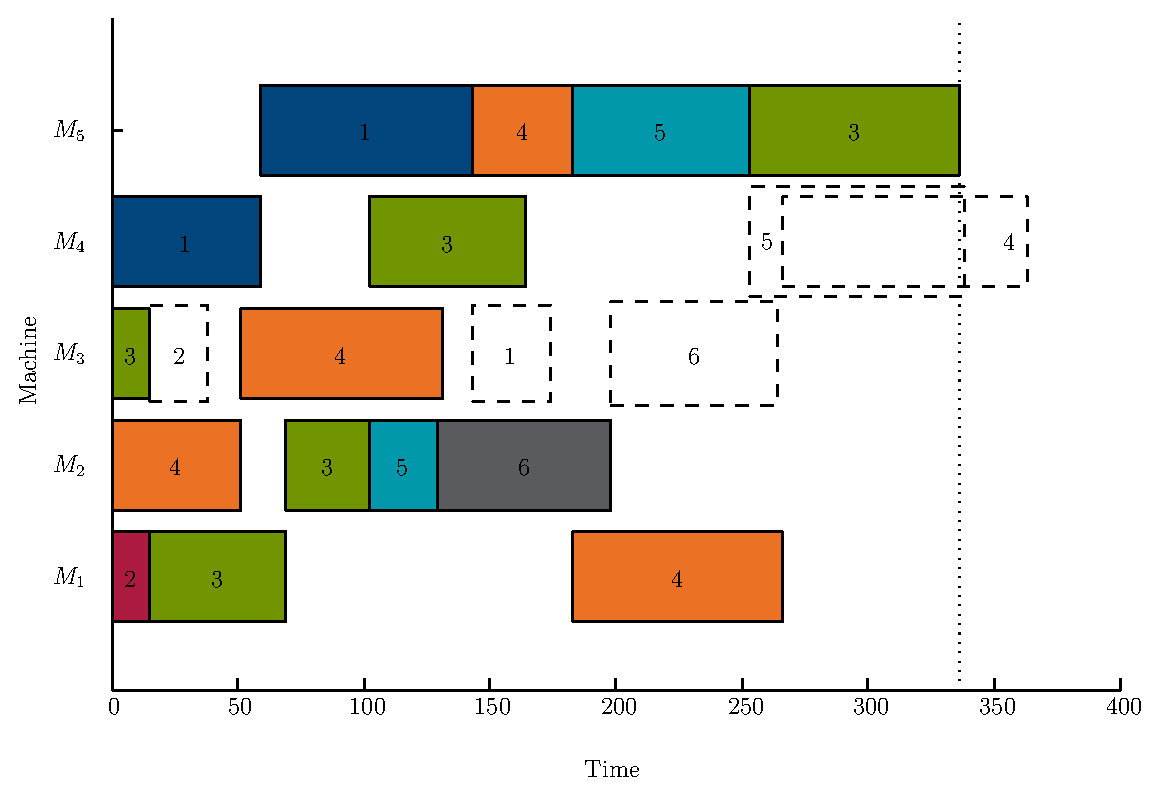
\includegraphics[width=\textwidth]{jssp_example}
\caption[Gantt chart of a partial \JSP\ schedule]{Gantt chart of a partial \JSP\ schedule after 15 dispatches: Solid and dashed boxes represent $\vchi$ and $\mathcal{R}^{(16)}$, respectively. Current $C_{\max}$ denoted as dotted line.}
\label{fig:example}
\end{figure}

\begin{figure}[p]\centering 
\noindent{\footnotesize\begin{tabbing}
\quad \quad \= 0\;\; \= \emph{Initialization}: Let $\vchi=\emptyset$ denote \\
\>  \> the current dispatching sequence. \\
\>1 \> {\bf for} \= $k := 1$ to $\ell=n\cdot m$ {\bf do} \emph{(at each dispatch iteration)}\\ 
\>2 \>\> {\bf for} \= $J_j\in \mathcal{R}^{(k)}\subset \mathcal{J}$ {\bf do} \emph{(inspect ready-list)} \\
\>3 \>\>\>  $I_j^{DR}\leftarrow \text{DR}\left([\vchi,j],Y\right)$ \emph{(priority $J_j$)}\\
\>4 \>\> {\bf od} \\
\>5 \>\> $j^*\leftarrow \argmax_{j\in \mathcal{R}^{(k)}}\{I_j^{DR}\}$ \emph{(choose highest priority)} \\
\>6 \>\> $\chi_k \leftarrow j^*$ \emph{(dispatch $j^*$)}\\
\>7 \> {\bf od} \\
\>8 \> $C_{max} \leftarrow Y(\vchi)$ \emph{(makespan)}
\end{tabbing}}
\caption{Pseudo code for constructing a \JSP\ sequence using a dispatching rule (DR) for a fixed construction heuristic (CH).}\label{fig:pseudocode}
\end{figure}


Henceforth, a \emph{sequence} will refer to the sequential ordering of the dispatches of tasks to machines, i.e., $(j,a)$; the collective set of allocated tasks to machines, which is interpreted by its sequence, is referred to as a \emph{schedule}; a \emph{scheduling policy} will pertain to the manner in which the sequence is manufactured for an (near) optimal schedule: be it a SDR such as MWR or via evolutionary search, etc. 

\section{Single-based priority dispatching rules}\label{sec:SDR}
\emph{Dispatching rules} (DR) are of a construction heuristics, where one starts with an empty schedule and adds sequentially on one operation (or task) at a time. Namely, at each time step $k$, an operation is dispatched which has the highest priority of the ready-list, \mbox{$\mathcal{R}^{(k)}\subset\mathcal{J}$}, i.e., the jobs who still have operations unassigned. If there is a tie, some other priority measure is used. 

A \emph{single-based priority dispatching rule}(SDR), or simple priority dispatching rule, is a function of features of the jobs and/or machines of the schedule. The features can be constant or vary throughout the scheduling process. For instance, the priority may depend on job processing attributes, such as which job has, 
\begin{description}
\item[Shortest immediate processing time (SPT)] \hfill \\
greedy approach to finish shortest tasks first,  
\item[Longest immediate processing time (LPT)] \hfill \\
greedy approach to finish largest tasks first, 
\item[Least work remaining (LWR)] \hfill \\
whose intention is to complete jobs advanced in their pro\-gress, i.e., minimising the ready-list $\mathcal{R}$,
\item[Most work remaining (MWR)] \hfill \\
whose intention is to accelerate the processing of jobs that require a great deal of work, yielding a balanced progress for all jobs during dispatching, however in-process inventory can be high.
\end{description}
These rules are the ones most commonly applied in the literature due to their simplicity and effectiveness, %\citep[cf.][]{Haupt89,Panwalkar77}
therefore they will be referenced throughout the dissertation. 
However there are many more available, e.g., randomly selecting an operation with equal possibility (RND); minimum slack time (MST); smallest slack per operation (S/OP); and using the aforementioned dispatching rules with predetermined weights. A survey of more than 100 of such rules are presented in \citet{Panwalkar77}, however the reader is referred to an in-depth survey for SDRs by \citet{Haupt89}. 

%Haupt89:
%Among the rules with job processing information, SPT is the most known, the most applied, and yet one of the most efficient rules. In line with LPT, it requires the lowest information amount, since only operation data (not job data) from the local queue (not from other queues) are needed.
%LWR give preference to jobs the work completed of which is rather advanced. Thus, they can be regarded as value-oriented rules selecting jobs with a high fraction of their value added or cumulative value to their total value.
% The intent of MWR is to speed up jobs with large processing work resulting in a well-balanced work progress of all jobs, at the expense of a high volume of in-process inventory, while LWR tend to reduce the number of jobs in the shop.

To summarise, SDRs assign an index to each job of the ready-list waiting to be scheduled, and are generally only based on few features and simple mathematical operations. 

%Haupt89:
%Among the rules with job processing information, SPT is the most known, the most applied, and yet one of the most efficient rules. In line with LPT, it requires the lowest information amount, since only operation data (not job data) from the local queue (not from other queues) are needed.
%LWR give preference to jobs the work completed of which is rather advanced. Thus, they can be regarded as value-oriented rules selecting jobs with a high fraction of their value added or cumulative value to their total value.
% The intent of MWR is to speed up jobs with large processing work resulting in a well-balanced work progress of all jobs, at the expense of a high volume of in-process inventory, while LWR tend to reduce the number of jobs in the shop.

\section{Features for \jsp}\label{sec:features}
A DR may need to perform a one-step look-ahead and observes features of the partial schedule to make a decision, for example by observing the resulting temporal makespan. These emanated observed features are sometimes referred to as an \emph{after-state} or \emph{post-decision state}. 

Features are used to grasp the essence of the current state of the schedule. Temporal scheduling features applied in this dissertation for a job $J_j$ to be dispatched on machine $M_a$ are given in \cref{tbl:features}. 
Note, from a job-oriented viewpoint, for a job already dispatched $J_j\in\mathcal{J}$ the corresponding set of machines now processed is $\mathcal{M}_j\subset\mathcal{M}$. Similarly from the machine-oriented viewpoint, $M_a\in\mathcal{M}$ with corresponding $\mathcal{J}_a\subset\mathcal{J}$. 

The features of particular interest were obtained from inspecting the aforementioned SDRs from \cref{sec:SDR}:  
\phiJobRelated\ and \phiMacRelated\ are job-related and machine-related attributes of the current schedule, respectively. 

Some features are directly observed from the partial schedule, such as the job- and machine-related features. 
In addition there are flow-related, \phiFlowRelated, which measure the influence of idle time on the schedule, 
and current makespan-related, \phiScheduleRelated.

Note that \phiLocalRelated\ are only based on the current step of the schedule, i.e., schedule's \emph{local features}, and might not give an accurate indication of how it will effect the schedule in the long run. Therefore, a set of features are needed to estimate the schedule's overall performance, referred to as its \emph{global features}. The approach here is to use well known SDRs, \phiSDRRelated, as a benchmark by retrieving what would the resulting $C_{\max}$ would be given if that SDR would be implemented from that point forward. Moreover, random completion of the partial schedule are implemented, here \phiRND\ corresponds to 100 random rollouts, which can be used to identify which features $\vphi$ are promising on a long-term basis.  

All of the features vary throughout the scheduling process, w.r.t. operation belonging to the same time step $k$, save for \phitotalProc\ which varies between jobs; \phistep\ to keep track of features' evolution w.r.t. the scheduling process; and \phiwrmTotal\ which is static for a given problem instance, but used for normalising other features, such as work-remaining based (\phiwrmJob\ and \phiwrmMac) or makespan-based (\phiGlobalRelated) ones.
In addition, \phimac, is reported in order to distinguish which features are in conflict with each other.

\begin{table} \centering 
  \caption[Feature space $\mathcal{F}$ for \JSP]{Feature space $\mathcal{F}$ for \JSP\ where job $J_j$ on machine $M_a$ given the resulting temporal schedule after dispatching $(j,a)$.}
  \label{tbl:features}
   {\footnotesize

 \centering
 \renewcommand{\arraystretch}{1.5}
  \begin{tabular}{clll} %p{0.45\textwidth}|p{0.4\textwidth}|}
   \toprule
$\vphi$ & Feature description & Mathematical formulation& Shorthand\\ 
%\hline  \multicolumn{4}{c}{\textbf{Local features}}  \\
\midrule
 \multicolumn{4}{c}{\textbf{job related}}\\
  \phiproc & job processing time & $p_{ja}$&proc\\
  \phistartTime & job start-time  & $x_s(j,a)$ &startTime\\
  \phiendTime & job end-time & $x_f(j,a)$ &endTime\\
  \phiarrivalTime & job arrival time &$x_f(j,a-1)$ & arrival\\ 
  \phitotalProc & total processing time & $\sum_{a\in \mathcal{M}}p_{ja}$ & totalProc\\
  \phiwait & time job had to wait &$x_s(j,a)-x_f(j,a-1) $ & wait\\   
  \phiwrmJob & total work remaining for job & $\sum_{a'\in\mathcal{M}\setminus \mathcal{M}_{j}}p_{ja'}$ & wrmJob\\
  \phijobOps & number of assigned operations for job & $|\mathcal{M}_j|$ & jobOps\\ 
\midrule
 \multicolumn{4}{c}{\textbf{machine related}}\\
  \phimacFree & when machine is next free & $\max_{j'\in \mathcal{J}_a} 
  \{x_f(j',a)\}$& macFree\\
  \phiwrmMac & total work remaining for machine &$\sum_{j'\in\mathcal{J}\setminus \mathcal{J}_{a}}p_{j'a} $ & wrmMac\\
  \phimacOps & number of assigned operations for machine & $|\mathcal{J}_a|$ & macOps\\
\midrule
 \multicolumn{4}{c}{\textbf{flow related}}\\
  \phislotsReduced & change in idle time by assignment & $\Delta s(a,j)$& slotsReduced \\
  \phislots & total idle time for machine & $\sum_{j'\in \mathcal{J}_a}s(a,j')$ & slots\\
  \phislotsTotal & total idle time for all machines & $\sum_{a'\in \mathcal{M}}\sum_{j'\in \mathcal{J}_{a'}}s(a',j')$  & slotsTotal\\
\midrule
 \multicolumn{4}{c}{\textbf{current makespan related}}\\
  \phimakespan & current makespan & $\max_{(j',a')\in \mathcal{J} \times \mathcal{M}_{j'}}\{x_f(j',a')\}$ & makespan \\
\midrule
 \multicolumn{4}{c}{\textbf{final makespan related}}\\
\phiSPT & final makespan using SPT & $ C_{\max}|\text{DR}=\text{SPT}$ & SPT \\
\phiLPT & final makespan using LPT  & $ C_{\max}|\text{DR}=\text{LPT}$ & LPT \\
\phiLWR & final makespan using LWR & $ C_{\max}|\text{DR}=\text{LWR}$ & LWR \\
\phiMWR & final makespan using MWR & $ C_{\max}|\text{DR}=\text{MWR} $ & MWR \\
\phiRND & final makespan using 100 random rollouts & $ \{C_{\max}|\text{DR}=\text{RND}\}_{i=1}^{100}$ & RND \\  
   \bottomrule
  \end{tabular}
}
 %Feature description for job $J_j$ on machine $M_a$ given current temporal schedule, where the set of jobs already dispatched are $J\subset\mathcal{J}$ on corresponding set of machines $\mathcal{M}_j\subset\mathcal{M}$

\end{table}



\section{Composite dispatching rules}\label{sec:CDR}
\citet{Jayamohan04} showed that a careful combination of dispatching rules can perform significantly better. These are referred to as \emph{composite dispatching rules} (CDR), where the priority ranking is an expression of several SDRs. For instance, optimising \JSP\ w.r.t. $L_{max}$ for one machine\ \cite[see. chapter 14.2]{Pinedo08}, one can combine SDRs that are optimal for a different criteria of problem instances, which complement each other as a CDR, e.g., combining the SDRs 
WSPT (SPT weighted w.r.t. $\mathcal{J}$), ``which is optimal when all release dates and due dates are zero,'' 
and minimum slack first (MS), ``which is optimal when all due dates are sufficiently loose and spread out,'' 
one gets the CDR apparent tardiness cost (ATC) which can work well on a broader set of problem instances than the original SDRs by themselves.

CDRs can deal with greater number of features and more complicated form, in short, CDR are a combination of several SDRs. For instance let CDR be comprised of $d$ SDRs, then the index $I$ for job $J_j$ using CDR is, 
\begin{equation}
I_j^{CDR} = \sum_{i=1}^d w_i \cdot \text{DR}^i(\vphi_j)
\end{equation}
where $w_i>0$ and $\sum_{i=0}^d w_i = 1$, then $w_i$ gives the \emph{weight} of the influence of $\text{DR}^i$ (which could be SDR or another CDR) to CDR. Note, each $\text{DR}^i$ is a function of the job $J_j$'s feature state $\vphi_j$.

\subsection{Blended dispatching rules}
Since each DR yield a priority index $I^{DR}$ then it is easy to translate its index as a  performance measure $a$, i.e., $a:~I^{DR}\mapsto \mathcal{Y}$. Then it is possible to combine several performance measures into a single DR, these are referred to as \emph{blended dispatching rules} (BDR), where an overall blended priority index $P$ is defined as 
\begin{equation}
P_j = \sum_{i=1}^d w_i \cdot a_i 
\end{equation}
where $w_i>0$ and $\sum_{i=0}^d w_i = 1$, then $w_i$ gives the weight of the proportional influence of performance measure $a_i$ (based on some SDR or CDR) to the overall priority. 

Generally the weights $\vec{w}$ chosen by the algorithm designer a priori. 
A more sophisticated approach would to learn have the algorithm discover these weights autonomously, for instance via evolutionary search or ordinal regression, to be discussed in \cref{ch:esmodels} and \cref{ch:prefmodels}, respectively.

\subsection{Automated discovery of dispatching rules}
\citet{Monch13} stress the importance of automated discovery of DRs and named several of successful implementations in the field of semiconductor wafer fabrication facilities. 
However, \citeauthor{Monch13} note that this sort of investigation is still in its infancy and subject for future research.

A recent editorial of the state-of-the-art approaches in advanced dispatching rules for large-scale manufacturing systems by \citet{Chen13} points out that:
\begin{quote}
[..] most traditional dispatching rules are based on historical data. With the emergence of data mining and on-line analytic processing, dispatching rules can now take predictive information into account.
\end{quote}
implying that there has not been much automation in the process of discovering new dispatching rules, which is the ultimate goal of this dissertation, i.e., automate creating optimisation heuristics for scheduling. 

With meta heuristics one can use existing DRs and use for example \textit{portfolio-based algorithm selection} \citep{Rice76,Gomes01}, either based on a single instance or class of instances \citep{Xu07} to determine which DR to choose from. 
Instead of optimising which algorithm to use under what data distributions, such as the case of portfolio algorithms, the approach taken in this dissertation is more similar to that of \emph{meta learning} \citep{Vilalta02} which is the study of how learning algorithms can be improved, i.e., exploiting their strengths and remedy their failings, in order for a better algorithm design. Thus creating an adaptable learning algorithm that dynamically finds the appropriate dispatching rule  to the data distribution at hand. 

\citet{Kalyanakrishnan11} point out that meta learning can be very fruitful in reinforcement learning, and in their experiments they discovered some key discriminants between competing algorithms for their particular problem instances, which provided them with a hybrid algorithm which combines the strengths of the algorithms.

\citet{Nguyen13} proposed a novel \textit{iterative dispatching rules} for \JSP\ which learns from completed schedules in order to iteratively improve new ones. At each dispatching step, the method can utilise the current feature space to `correctify' some possible `bad' dispatch made previously (sort of reverse lookahead).
Their method is straightforward, and thus easy to implement and more importantly, computationally inexpensive, although \citeauthor{Nguyen13} stress that there still remains room for improvement. 

\citet{Korytkowski13} implemented \textit{Ant Colony Optimisation} to select the best DR from a selection of nine DRs for \JSP\ and their experiments showed that the choice of DR do affect the results and that for all performance measures considered it was better to have all of the DRs to choose from rather than just a single DR at a time. 
Similarly, \citet{Lu13} investigate eleven SDRs for \JSP\ to create a pool of thirty three CDRs that strongly outperformed the ones they were based on, which is intuitive since where one SDR might be failing, another could be excelling, hence combining them should yield a better CDR. \citeauthor{Lu13} create their CDRs with \textit{multi-contextual functions} based either on machine idle time or job waiting time, so one can say that the CDRs are a combination of those two key features of the schedule and then the basic DRs. However, there are no combinations of the basic DR explored, only machine idle time and job waiting time.  
\citet{Yu13} used priority rules to combine twelve existing DRs from the literature, in their approach they had forty eight priority rules combinations, yielding forty eight different models to implement and test. This is a fairly ad hoc solution and there is no guarantee the optimal combination of DRs is found. 

\clearpage
\section{Rice's framework for \jsp}\label{sec:rice:jsp}
\citeauthor{Rice76}'s framework for algorithm selection (discussed in \cref{sec:rice}) has already been formulated for \jsp\ \citep[cf.][]{SmithMilesLion3,SmithMilesLion5,InRu12}, as follows, 
\begin{description} 
\item[Problem space] $\mathcal{P}$ is defined as the union of $N$ problem instances consisting of processing time and ordering matrices,
\begin{equation} 
\mathcal{P}=\left\{(p_{ja}^{(i)},\vsigma_j^{(i)})\;\big|\;J_j\in\mathcal{J},\;M_a\in\mathcal{M}\right\}_{i=1}^{N}
\end{equation}
Problem generators for $\mathcal{P}$ are given in \cref{ch:genprobleminstances}.
\item[Feature space] $\mathcal{F}$ which is outlined in \cref{sec:features}. Note, these are not the only possible set of features, however, the local feature, \phiLocalRelated, are built on the work by \cite{InRu11a,SmithMilesLion3} and deemed successful in capturing the essence of a \jsp\ data structure;
\item[Algorithm space] $\mathcal{A}$ is simply the scheduling policies under consideration, e.g., SDRs from \cref{sec:SDR},
\begin{equation}
\mathcal{A}=\left\{\text{SPT,~LPT,~LWR,~MWR,~}\dotsc\right\}
\end{equation} 
\item[Performance space] $\mathcal{Y}$ is based on the resulting $C_{\max}$, defined by \cref{eq:makespan}. The optimum makespan is denoted $C_{\max}^{\text{opt}}$, and the makespan obtained from the scheduling policy $A\in\mathcal{A}$ under inspection by $C_{\max}^{A}$. Since the optimal makespan varies between problem instances the performance measure is the following, 
\begin{equation}\label{eq:rho}
\rho=\frac{C_{\max}^{A}-C_{\max}^{opt}}{C_{\max}^{\text{opt}}}\cdot 100\%
\end{equation}
which indicates the \namerho. Thus $\mathcal{Y}$ is the following, 
\begin{equation}
\mathcal{Y}=\left\{\rho_i\right\}_{i=1}^{N}
\end{equation}
\end{description}
The mapping $Y:\;\mathcal{A}\times\mathcal{F} \mapsto \mathcal{Y}$ is the step-by-step construction heuristic introduced in \cref{sec:CH}.
\include{chapters/genprobleminstances}
\HeaderQuote{Sentence first -- verdict afterwards.}{The Queen}

\chapter{Problem Structure}\label{ch:problemstructure} 

%\begin{abstract} 
%Many heuristic methods have been proposed for the \jsp\ scheduling problem. Different solution methodologies outperform other depending on the particular problem instance under consideration. Therefore, one is interested in knowing how the instances differ in structure and determine when a particular heuristic solution is likely to fail and explore in further detail the causes. In order to achieve this, we seek to characterise features for different difficulties. Preliminary experiments show there are different significant features that distinguish between easy and hard \jsp\ problem, and that they vary throughout the scheduling process. 
%The insight attained by investigating the relationship between problem structure and heuristic performance can undoubtedly lead to better heuristic design that is tailored to the data distribution under consideration.
%\end{abstract}


\FirstSentence{P}{roblem structure and heuristic effectiveness} are closely intertwined. When investigating the relation between the two, one can research what \citet{Corne10} call \emph{footprints} in instance space, which is an indicator how an algorithm generalises over a given instance space. This sort of investigation has also been conducted by \citet{Pfahringer00} under the alias \emph{landmarking}. 
% quote Corne10: ``such a footprint indicates how an algorithm's comparative performance generalises in instance space''
% quote Katie2009: ``Landmarking tries to directly characterise a domain by relating the performance to some learners -- the landmarkers -- to the performance of some other algorithm.''
From experiments performed by \citeauthor{Corne10}, it is evident that one-algorithm-for-all problem instances is not ideal, in accordance with no free lunch theorem \citep{Wolpert97nofree}. An algorithm may be favoured for its best overall performance, however it is rarely the best algorithm available over various subspaces of the instance space.
Therefore, when comparing different algorithms one needs to explore how they perform w.r.t. the instance space, i.e., their footprint. That is to say, one can look at it as finding which footprints correspond to a subset of the instance space that works \emph{well} for a given algorithm, and similarly finding which footprints correspond to a subset of the instance space that works \emph{poorly} for a given algorithm. 

In the context of \jsp\ this corresponds to finding \emph{good} (makespan close to its optimum)  and \emph{bad} (makespan far off its optimum) schedules. Note, good and bad schedules are interchangeably referred to as \emph{easy} and \emph{hard} schedules (pertaining to the manner they are achieved), respectively. 

\citet{SmithMilesLion5} also investigate algorithm performance in instance space using footprints. The main difference between \citeauthor{Corne10} and \citeauthor{SmithMilesLion5} is how they discretise the instance space. In the case of \citeauthor{Corne10} they use \jsp\ and discretise manually between different problem instances; on one hand w.r.t. processing times, e.g.,  $\vec{p}\sim \mathcal{U}(10,20)$ versus $\vec{p}\sim \mathcal{U}(20,30)$ etc., and on the other hand w.r.t. number of jobs, $n$. 
They warn that footprinting can be uneven, so great care needs to be taken in how to discretise the instance space into subspaces. 
On the other hand, \citeauthor{SmithMilesLion5} use a completely automated approach. Using timetabling instances, they implement a self-organizing map to group similar problem instances together, that were both real world instances and synthetic ones using different problem generators. 

Going back to the \jsp\ paradigm, then the interaction between processing time distribution and its permutation is extremely important, because it introduces hidden properties in the data structure making it \emph{easy} or \emph{hard} to schedule for the given algorithm. These underlying characteristics, i.e., features, define its data structure. A more sophisticated way of discretising the instance space is grouping together problem instances that show the same kind of feature behaviour, especially given the fact the learning models in \cref{ch:prefmodels} will be heavily based on feature pairs. Thereby making it possible to infer what sort of feature behaviour distinguishes  between \emph{good} and \emph{bad} schedules. 

In \citet{InRu12}, a single problem generator was used to create  $N=1,500$ synthetic $6\times6$ \jsp\ problem instances, where $\vec{p}\sim\mathcal{U}(1,200)$ and $\vsigma$ was a random permutation. The experimental study showed that MWR works either well or poorly on a subset of the instances, in fact 18\% and 16\% of the instances were classified as \emph{easy} and \emph{hard} for MWR, respectively. 
Since the problem instances were na\"{i}vely generated, not to mention given the high variance of the data distribution, it is intuitive that there are some inherent structural qualities that could explain this difference in performance. The experimental study investigated the feature behaviours for these two subsets, namely, the easy and hard problem instances. For some features, the trend was more or less the same, which are explained by the common denominating factor, that all instances were sampled from the same problem generator. Whereas, those features that were highly correlated with the end-result, i.e., the final makespan, which determined if an instance was labelled easy or hard, then the significant features varied greatly between the two difficulties, which imply the inherent difference in data structure. 
Moreover, the study in gives support to that random problem instance generators are \emph{too} general and might not suit real-world applications. \citet{Whitley} argue that problem instance generator should be more structured, since real-world manufacturing environment is not completely random, but rather structured, e.g.,  job's tasks can be correlated or machines in the shop. \citeauthor{Whitley} propose a problem instance generator that relates to real-world \fsp\ attributes, albeit not directly modelled after real-world \fsp\ due to the fact that deterministic $Fm||C_{\max}$ is seldom directly applicable in practice \citep{Dudek92}. This is why \fjc{n}{m}, \fmc{n}{m} and \fmxc{n}{m} are also taken into consideration in \cref{ch:genprobleminstances} as they are an attempt to mimic the real-world characteristics of \fsp.

It is interesting to know if the difference in the structure of the schedule is time dependent, e.g.,  is there a clear time of divergence within the scheduling process? 
Moreover, investigation of how sensitive is the difference between two sets of features, e.g.,  can two schedules with similar feature values yield completely contradictory outcomes (i.e. one poor and one good schedule)? Or will they more or less follow the their predicted trend? If the latter is the prevalent case, then these instances need to be segregated and each having their own learning algorithm implemented, for a meaningful outcome overall.  
This also, essentially, answers the question of whether  it is in fact feasible to discriminate between \emph{good} and \emph{bad} schedules using the currently selected features as a measure. If results are contradictory, it is an indicator the features selected are not robust enough to capture the essence of the data structure and some key features are missing from the feature set that could be able to discriminate between \emph{good} and \emph{bad} schedules. 
Additionally, there is also the question of how can one define ``similar'' schedules, and what measures should be used? This \lcnamecref{ch:problemstructure} describes some preliminary experiments with the aim of investigating the feasibility of finding distinguishing features corresponding to \emph{good} and \emph{bad} schedules in \jsp. To summarise:
\begin{inparaenum}[(a)]
	\item How to define problem difficulty? 
	\item Is there a time of divergence?
	\item What are ``similar'' schedules?
	\item Do similar features yield contradictory outcomes?
	\item Are extra features needed? 
	And \item what can be learned from feature behaviour?
\end{inparaenum}

Instead of searching through a large set of algorithms  and determining which algorithm is the most suitable for a given subset of the instance space, i.e., creating an algorithm portfolio, as is generally the focus in the current literature \citep{SmithMilesLion3,SmithMilesLion5,Corne10}, the focus of the experimental study in \cref{sec:diff:jrnd,sec:diff:jrndn,sec:diff:frnd,sec:diff:frndn,sec:diff:fjc,sec:diff:fmc,sec:diff:fmxc} 
(each corresponding to a given problem space from \cref{ch:genprobleminstances})
is rather on few simple algorithms, here the SDRs described in \cref{sec:SDR}, and understanding \emph{how} they work on the instance space, similar to \citet{Whitley}, who analyse the fitness landscape of several problem classes for a fixed algorithm. 
Note, figures and tables that accompany this \lcnamecref{ch:problemstructure} are mostly located in \cref{app:problemstructure}.


\section{Distribution difficulty w.r.t. SDRs}
Depending on the data distribution, dispatching rules perform differently. Take for instance the common single-based priority dispatching rules; SPT, LPT, LWR and MWR (cf. \cref{sec:SDR}). 
A box-plot for \fullnamerho, for all problem spaces in \cref{ch:genprobleminstances} are depicted in \cref{fig:SDR:boxplot}. 
As one can see, there is a staggering difference between the interaction of SDRs and their problem space. MWR is by far the best out of the four SDRs inspected for \JSP\ -- not only does it reach the known optimum most often but it also has the lowest worst-case factor from optimality. Similarly LWR for \FSP.
Although the same processing time distribution is used, there are some inherent structure in which MWR and LWR can exploit for \JSP\ and  \FSP, respectively, whereas the other SDRs cannot. However, \emph{all} of these dispatching rules are considered good and commonly used in practice and no one is better than the rest \citep{Haupt89}, it simply depends on the data distribution at hand. This indicates that some distributions are harder than others, and these \JSP\ problem generators simply favours MWR, whereas the \FSP\ problem generators favours LWR. 

\section{Experimental settings}
% Katie orðar: A correlation analysis between the feature space and the performance space was conducted across all 1,500 problem instances revealed that instance features that appear to correlate (linearly) with heuristic performance are $phi(?)$ (correlation $=-0.59$) and $phi(?)$ (correlation $=0.44$). None of the other instance features appear to have a linear relationship with algorithmic performance.

The main focus is on knowing \emph{when} during the scheduling process easy and hard problems diverge and explore in further detail \emph{why} they diverged. Rather than visualising high-dimensional data projected onto two dimensional space (as was the focus in \cite{SmithMilesLion5} with self-organising maps), instead appropriate statistical tests with a significance level $\alpha=0.05$ is applied to determine if there is any difference between different data distributions. For this the two-sample Kolmogorov–Smirnov test (K-S test) is used to determine whether two underlying one-dimensional probability distributions differ. 
Furthermore, in order to find defining characteristics for easy or hard problems, a (linear) correlation is computed between features to the resulting \namerho.

Note, when inspecting any statistical difference between data distribution of the features on a step by step basis, the features at step $k+1$ are of course dependant on all previous $k$ steps. This results in repetitive statistical testing, therefore a Bonferroni adjustment is used to counteract the multiple comparisons, i.e., each stepwise comparison has the significant level $\alpha_k=\frac{\alpha}{\ell}$, and thus maintaining the $\sum_{k=1}^{\ell}\alpha_k=\alpha$ significance level.

\section{Defining `easy' versus `hard' schedules}\label{sec:diff:easyhard}
It's relatively ad-hoc how to define what makes a schedule difficult. Intuitively, it's logical to use the schedule's objective to define it directly, i.e., inspecting \fullnamerho. Moreover, since the SDRs from \cref{sec:SDR} will be used throughout as a benchmark for subsequent models, the quantiles for \namerho, using the SDRs on their training set will be used to differentiate between easy and hard scheduling problems. In particular, the classification is defined as follows, 
\begin{description}
	\item[Easy] schedules belong to the first quantile, i.e., \hfill \\
	\begin{equation}\label{eq:easy}
		\mathcal{E}(a):=\{\vec{x}\;|\;\rho=Y(a,\vec{x})<\rho^{\text{1st. Qu.}}\}
	\end{equation} 
	\item[Hard] schedules belong to the third quantile, i.e., \hfill \\
	\begin{equation}\label{eq:hard}
		\mathcal{H}(a):=\{\vec{x}\;|\;\rho=Y(a,\vec{x})>\rho^{\text{3rd. Qu.}}\}
	\end{equation} 
\end{description}
where $\vec{x}\in\mathcal{P}_{\text{train}}$ for a given dispatching rule $a\in\mathcal{A}:=\{\text{SPT,~LPT,~LWR,~MWR}\}$.

\Cref{tbl:easyhard:quantile} reports the first and third quantiles for each problem space, i.e., the cut-off values that determine the SDRs difficulty, whose division, defined as percentage of problem instances, i.e., 
\begin{equation}\label{eq:easyhard:cnt}
	\frac{\abs{\mathcal{E}(a)}}{N_{\text{train}}} \cdot 100\%
	\quad \text{and} \quad 
	\frac{\abs{\mathcal{H}(a)}}{N_{\text{train}}}\cdot 100\%
\end{equation}
for each $a\in\mathcal{A}$, are given in \cref{tbl:easyhard:cnt:6x5,tbl:easyhard:cnt:10x10}, respectively. 

\section{Consistency of problem instances}
The intersection of pairwise SDRs being simultaneously easy or hard are given in \cref{tbl:easy:cnt:6x5,tbl:easy:cnt:10x10,tbl:hard:cnt:6x5,tbl:hard:cnt:10x10}, i.e., 
\begin{equation}\label{eq:easyorhard:cnt}
	\frac{\abs{\mathcal{E}(a_i)\cap \mathcal{E}(a_j) }}{N_{\text{train}}} \cdot 100\%
	\quad \text{or} \quad 
	\frac{\abs{\mathcal{H}(a_i)\cap \mathcal{H}(a_j)}}{N_{\text{train}}}\cdot 100\%
\end{equation}
where $a_i,a_j\in\mathcal{A}$. Note, when $a_i=a_j$ then \cref{eq:easyorhard:cnt} is equivalent to \cref{eq:easyhard:cnt}.

Even though this is a na\"ive way to inspect difference between varying SDRs, it's does give some initial insight of the potential of improving dispatching rules; a sanity check before going into extensive experiments, as will be done in \cref{sec:diff:stepwise}.

For the corresponding $10\times10$ training set (cf. \cref{tbl:easy:cnt:10x10,tbl:hard:cnt:10x10}), the intersections between SDRs from $6\times5$ (cf. \cref{tbl:easy:cnt:6x5,tbl:hard:cnt:6x5}) seem to hold. 
However, by going to a higher dimension, the performance edge between SDRs becomes more apparent, e.g., in \JSP\ when there was a slight possibility of LWR being simultaneously easy as other SDRs ($5\%<$ chance), it becomes almost impossible for $10\times10$. 
Making LWR a clear underdog. 
Despite that, for \FSP\ the tables turn; now LWR has the performance edge. 
For instance, for \frndn{6}{5} the second  best option is to apply LPT (13.22\%), however there is a quite high overlap with LWR (11.74\%), and since LWR is easier significantly more often (85.18\%), the choice of SDR is quite obvious. 
Although, it goes to show that there is the possibility of improving LWR by sometimes applying LPT-based insight; by seeing what sets apart the intersection of their easy training sets. 

Similarly for every $10\times10$ \JSP\ (cf. \cref{tbl:easy:cnt:10x10}), almost all easy LPT schedules are also easy  for MWR ($<1\%$ difference), as is to be expected as MWR is the more sophisticated counterpart for LPT (like LWR is for SPT). 
However, the greedy approach here is  not gaining any new information on how to improve MWR. 
In fact, MWR is never considered hard for any of the \JSP\ (cf. \cref{tbl:hard:cnt:10x10}), therefore no intersection with any hard schedules. 
But the LPT counterpart has a relatively high occurrence rate (3-14\%), so due to the similarity of the dispatching rules, the denominating factor between LPT and MWR can be an indicator for explaining some of MWR's pitfalls.
That is to say, why aren't all of the \jsp\ schedules easy when applying MWR? 

These have up until now all been speculations about how SDRs differ. One thing is for certain, the underlying problem space plays a great role on a SDR's success. Even slight variations to one job or machine, i.e., \jrndJ{10}{10} and \jrndM{10}{10}, shows significant change in performance. Due to the presence of bottleneck, MWR is able to detect it and thus becomes the clear winner. Even outperforming the original \jrnd{10}{10} which they're based on, despite having processing times doubled for a single job or machine, with approximately 10\% lower first quantile (cf. \cref{tbl:easyhard:quantile:10x10}) in both cases. 

As the objective of this dissertation is not to choose which DR is best to use for each problem instance. 
The focus is set on finding what characterises of \jsp\ overall, are of value (i.e. feature selection), and create a new model that works well for the problem space to a great degree.
Namely, by exploiting feature behaviour that is considered more favourable. The hypothesis being that features evolutions of easy schedules greatly differ from features evolutions corresponding to hard schedules, and \cref{sec:diff:stepwise} will attempt to explain the evidence show in \cref{tbl:easyhard:cnt:6x5,tbl:easyhard:cnt:10x10,tbl:easy:cnt:6x5,tbl:easy:cnt:10x10,tbl:hard:cnt:6x5,tbl:hard:cnt:10x10}.

Note, this \lcnamecref{sec:diff:easyhard} gave the definition of what constitutes an `easy' and `hard' schedule. Since these are based on four SDRs, $\mathcal{A}$, the training data for the experiments done in this \lcnamecref{ch:problemstructure} is based on $4N_{\text{train}}$ problem instances, per problem space, therefore,
\begin{equation}\label{eq:easyhard:all}
	\sum_{a\in\mathcal{A}}\abs{\mathcal{E}(a)} \approx N_{\text{train}}
	\quad\text{and}\quad
	\sum_{a\in\mathcal{A}}\abs{\mathcal{H}(a)} \approx N_{\text{train}}
\end{equation} 
due to the fact \cref{eq:easy,eq:hard} are based on the first and third quantiles of the entire training set.
Now, as the SDRs vary greatly in performance, the contribution of a SDR to \cref{eq:easyhard:all} varies, resulting in an unbalanced sample size when restricted to a single SDR. 

\section{Probability of choosing optimal decision}\label{sec:diff:opt:rnd}
In order to create successful dispatching rules, a good starting point is to investigate the properties of optimal solutions and hopefully be able to learn how to mimic such `good' behaviour. 
For this, we follow an optimal solution,\footnote{Optimal solutions are obtained by using a commercial software package \cite{gurobi}.} and inspect the evolution of its features  (defined in \cref{tbl:features}) throughout the dispatching process. 
Moreover, it is noted, that there are several optimal solutions available for each problem instance. However, it is deemed sufficient to inspect only one optimal trajectory per problem instance as there are $N_{\text{train}}$ independent instances which gives the training data variety. 


Firstly, we can observe that on a step by step basis there are several optimal dispatches to choose from. \Cref{fig:diff:opt:unique} depicts how the number of optimal dispatches evolve at each dispatch iteration. Note, that only one optimal trajectory is pursued (chosen at random), hence this is only a lower bound of uniqueness of optimal solutions.
As the number of possible dispatches decrease over time, \cref{fig:diff:opt} depicts the probability of choosing an optimal dispatch at each iteration. 

\section{Making suboptimal decisions}\label{sec:diff:opt:sub}
Looking at \cref{fig:diff:opt}, \jrnd{10}{10} has a relatively high probability ($70\%$ and above) of choosing an optimal job. However, it is imperative to keep making optimal decisions, because once off the optimal track the consequences can be dire. To demonstrate this interaction \cref{fig:diff:case} depicts the worst and best case scenario of \namerho, once you've fallen off the optimal track. Note, that this is given that you make \emph{one} wrong turn. Generally, there will be many mistakes made, and then the compound effects of making suboptimal decisions really start adding up. 

It is interesting that for \JSP, that over time making suboptimal decisions make more of an impact on the resulting makespan. This is most likely due to the fact that if a suboptimal decision is made in the early stages, then there is space to rectify the situation with the subsequent dispatches. However, if done at a later point in time, little is to be done as the damage is already been inflicted upon the schedule. 
However, for \FSP, the case is the exact opposite. Under those circumstances it's imperative to make good decisions right from the beginning. This is due to the major structural differences between \jsp\ and \fsp, namely the latter having a homogeneous machine ordering, constricting the solution immensely. Luckily, this does have the added benefit of making \fsp\ less vulnerable for suboptimal decisions later in the decision process. 


\section{Optimality of simple priority dispatching rules}\label{sec:diff:opt:sdr}
The probability of optimality of the aforementioned SDRs from \cref{sec:SDR}, yet still maintaining our optimal trajectory, i.e., the probability of a job chosen by a SDR being able to yield an optimal makespan on a step by step basis, is depicted  in   \cref{fig:diff:opt:SDR}. Moreover, the dashed line represents the benchmark of randomly guessing the optimum (cf. \cref{fig:diff:opt}).

Now, let's bare in mind \namerho, of applying SDRs throughout the dispatching process (cf. box-plots of which in \cref{fig:SDR:boxplot}), then there is a some correspondence between high probability of stepwise optimality and low $\rho$. Alas, this isn't always the case, for \jrnd{10}{10} SPT always outperforms LPT w.r.t. stepwise optimality, however this does not transcend to SPT having a lower $\rho$ value than LPT. Hence, it's not enough to just learn optimal behaviour, one needs to investigate what happens once we encounter suboptimal state spaces.

\section{Simple blended dispatching rule}\label{sec:diff:opt:bdr}
As stated before, the goal of this \lcnamecref{ch:problemstructure} is to utilise feature behaviour to motivate new, and \emph{hopefully} better, dispatching rules. 
A na\"ive approach would be creating a simple blended dispatching rule which would be for instance switch between two SDRs at a predetermined time point. Hence, going back to \cref{fig:diff:opt:SDR} a presumably good BDR for \jrnd{10}{10}  would be starting with SPT and then switching over to MWR at around time step $k=40$, where the SDRs change places in outperforming one another. A box-plot for \namerho, for all $10\times10$ problem spaces is depicted in \cref{fig:diff:boxplot:BDR}. This little manipulation between SDRs does outperform SPT immensely, yet doesn't manage to gain the performance edge of MWR, save for \frnd{10}{10}. This gives us insight that for \jsp, the attribute based on MWR is quite fruitful for good dispatches, whereas the same cannot be said about SPT -- a more sophisticated BDR is needed to improve upon MWR. 

A reason for this lack of performance of our proposed BDR is perhaps that by starting out with SPT in the beginning, it sets up the schedules in such a way that it's quite greedy and only takes into consideration jobs with shortest immediate processing times. Now, even though it is possible to find optimal schedules from this scenario, as \cref{fig:diff:opt:SDR} shows, the inherent structure is already taking place, and might make it hard to come across optimal moves by simple methods. Therefore it's by no means guaranteed that by simply swapping over to MWR will handle the situation that applying SPT has already created. \Cref{fig:diff:boxplot:BDR} does however show, that by applying MWR instead of SPT in the latter stages, does help the schedule to be more compact w.r.t. SPT. However, in the case of \jrnd{10}{10} and \jrndn{10}{10} the fact remains that the schedules have diverged too far from what MWR would have been able to achieve on its own. Preferably the blended dispatching rule should use  best of both worlds, and outperform all of its inherited DRs, otherwise it goes without saying, one would simply still use the original DR that achieved the best results.

\begin{figure}
	\centering
	\includegraphics[width=1\linewidth]{figures/{boxplotRho.BDR.10x10}.pdf}
	\caption{Box plot for \namerho, for BDR where SPT is applied for the first 40\% of the dispatches, followed by MWR.}
	\label{fig:diff:boxplot:BDR}
\end{figure}

\section{Extremal feature}\label{sec:diff:opt:ext}
The SDRs we've inspected so-far are based on two features from \cref{tbl:features}, namely, 
\begin{inparaenum}[(i)]
	\item \phiproc\ for SPT and LPT, and
	\item \phiwrmJob\ for LWR and MWR. 
\end{inparaenum}
By choosing the lowest value for the first SDR, and highest value for the latter SDR, i.e., the extremal values for those given features. Let's apply the same methodology from \cref{sec:diff:opt:sdr} to all varying features\footnote{Note, \phistep, \phimac\ and \phiwrmTotal\ describe the features, not the schedule. For instance, \phistep\, gives us no new information, as that feature is homogeneous for each time step, making it equivalent to random guessing.} described in \cref{tbl:features}. 
\Cref{fig:diff:opt:minmax}
depict the probability of all extremal features being an optimal dispatch, with random guessing from \cref{fig:diff:opt} as a dashed line. \todo[inline]{Discuss more?}

\section{Feature evolution}\label{sec:diff:opt:evol}
In order to put the extremal features into perspective, it's worth comparing them with how the evolution of the features are over time, depicted in \cref{fig:diff:opt:evol}. 


\section{Emergence of problem difficulty}\label{sec:diff:stepwise}


\section{Structure of problem spaces}
Up till now the discussion has been general and covering many problem spaces simultaneously. The subsequent \lcnamecref{sec:diff:jrnd}s will go into more depth what is going on per individual problem space.  
\subsection{\Jrnd}\label{sec:diff:jrnd}
\subsection{\Jrndn}\label{sec:diff:jrndn}
\subsection{\Frnd}\label{sec:diff:frnd}
\subsection{\Frndn}\label{sec:diff:frndn}
\subsection{\Fjc}\label{sec:diff:fjc}
\subsection{\Fmc}\label{sec:diff:fmc}
\subsection{\Fmxc}\label{sec:diff:fmxc}

\section{Discussion and Conclusion}
Despite problem instances being created by the same problem generator, they vary among one another enough. As a result, all instances are not created equal; some are always hard to solve, others always easy. 
Since the description of the problem space isn't enough to predict its performance, we need a measure to understand what's going on. Why are some instances easier to find their optimum (or close enough)? That is to say, what's their secret? This is where their feature evolution comes into play.
By using schedules obtained by applying SDRs we have the ability to get some insight into the matter. 

From the experimental study it is apparent that features have different %impact 
correlation with the resulting schedule depending in what stage it is in the scheduling process, implying that their influence varies over the dispatching sequencing. Moreover, features constant throughout the scheduling process are not correlated with the end-result.
There are some common features for both difficulties considered which define \jsp\ on a whole. However the significant features are quite different across the two difficulties, implying there is a clear difference in their data structure. The amount of significant features were considerably more for easy problems, indicating their key elements had been found. However, the features distinguishing hard problems were scarce. Most likely due to their more complex data structure their key features are of a more composite nature. As a result, new `global' features were introduced. 

It is possible for a \JSP\ schedule to have more than one sequential dispatching representation. It is especially w.r.t. the initial dispatches. Visiting \cref{fig:example} again, if jobs $J_j\in\{J_1,J_2,J_6\}$ were to be dispatched first, then all permutations yield the same equivalent temporal schedule, this is because they don't create a conflict for one another (as is the case for jobs $J_4$ and $J_5$). This drawback of non-uniqueness of sequential dispatching representation explains why there is hardly any significant feature for the initial steps of the scheduling process (cf. \cref{tbl:JSP:feat:easy} and \cref{tbl:JSP:feat:hard}). 

Since feature selection is of paramount importance in order for algorithms to become successful, one needs to give great thought to how features are selected. What kind of features yield \emph{bad} schedules? And can they be steered onto the path of more promising feature characteristics. This sort of investigation can be an indicator how to create meaningful problem generators. On the account that real-world problem instances are scarce, their hidden properties need be drawn forth in order to generate artificial problem instances from the same data distribution. 

The feature attributes need to be based on statistical or theoretical grounds. 
Scrutiny in understanding the nature of problem instances therefore becomes of paramount importance in feature engineering for learning, as it yields feedback into what features are important to devote more attention to, i.e., features that result in a failing algorithm. 
For instance, in \cref{tbl:JSP:feat:same} the slack features have the same distribution in the initial stages of the scheduling process, however there is a clear point of divergence which needs to be investigate why the sudden change? 
In general, this sort of investigation can undoubtedly be used in better algorithm design which is more equipped to deal with varying problem instances and tailor to individual problem instance's needs, i.e., a footprint-oriented algorithm. 

Although this methodology was only implemented on a set of simple single-priority dispatching rules, the methodology is easily adaptable for more complex algorithms, such as the learned preference models in \cref{sec:pref:problemstructure}. The main objective of this work is to illustrate the interaction of a specific algorithm on a given problem structure and its properties. 
%\include{chapters/prefmodels}
\HeaderQuote{There's a large mustard-mine near here. And the moral of that is -- The more there is of mine, the less there is of yours.}{The Duchess} 


\chapter{Evolutionary learning of CDRs}\label{ch:esmodels} \todo[color=green!40,noline]{\cref{ch:esmodels} Unfinished, taken from GECCO submission}

%Evolutionary learning of weighted linear composite dispatching rules for scheduling

\FirstSentence{G}{enetic algorithms (GA) are one of the} most widely used approaches in \JSP\ literature \citep{Pinedo08}. However, in that case an extensive number of schedules need to be evaluated, and even for low dimensional \JSP\ that can quickly become computationally infeasible.
GAs can be used directly on schedules \citep{Cheng96,Cheng99,Tsai07,Qing-dao-er-ji12,Ak12,Meeran12}, however, in that case there are many concerns that need to be dealt with. To begin with there are nine encoding schemes for representing the schedules \cite{Cheng96}, in addition there has to be special care when applying cross-over and mutation operators in order for the schedules, now in the role of `chromosomes,' to still remain feasible. Moreover in case of \JSP\ the GAs are not adapt for fine-tuning around optima, luckily a subsequent local search can mediate the optimisation \citep{Cheng99,Meeran12}.

Another approach is to apply GAs indirectly to \JSP , via dispatching rules, i.e., Dispatching Rules Based Genetic Algorithms (DRGA) \citep{Vazquez-Rodriguez09,Dhingra10,Nguyen13} where a solution is no longer a \emph{proper} schedule but a \emph{representation} of a schedule via applying certain dispatching rules consecutively. 
DRGA are a special case of \emph{genetic programming} \citep{Koza05} which is the most predominant approach in hyper-heuristics is a framework of creating \emph{new} heuristics from a set of  predefined heuristics via GA optimisation \citep{Burke10}. 

A prevalent approach to solving \JSP\ is to combine several relatively simple dispatching rules such that they may benefit each other for a given problem space. Generally, this is done on an ad-hoc basis, requiring expert knowledge from heuristics designer, or extensive exploration of suitable combinations of heuristics. The approach in this \namecref{ch:esmodels}, is to automate that selection, by translating dispatching rules into measurable features and optimising what their contribution should be via evolutionary search. The framework is straight forward and easy to implement and shows promising results. Various data distributions from \cref{ch:genprobleminstances} are investigated, however only trained on the lower dimension, $6\times5$, yet, validated on higher dimension, $10\times10$. 

Moreover, \cref{sec:es:measure} shows that the choice of objective function  for evolutionary search is worth investigating. Since the optimisation is based on minimising the expected mean of the fitness function over a large set of problem instances, which can vary within. Then normalising the objective function can stabilise the optimisation process away from local minima. 

\section{Introduction}
As previously discussed in \cref{ch:introduction}, there are two main viewpoints on how to approach scheduling problems,
\begin{inparaenum}[\itshape a\upshape)] 
\item local level by building schedules for one problem instance at a time;
and \item global level by building schedules for all problem instances at once.
\end{inparaenum}
\tcr{For local level construction a simple construction heuristic is applied, the schedule's features are collected at each dispatch iteration, from which a learning model will inspect the feature set to discriminate which operations are preferred to others via ordinal regression. The focus is essentially on creating a meaningful preference set composed of features and their ranks, as the learning algorithm is only run once to find suitable operators for the value function. This is the approach taken in \cite{InRu11a}.} Expanding on that  work, this study will explore global level construction viewpoint, where there is no feature set collected beforehand since the learning model is optimised directly via evolutionary search. This requires numerous costly value function evaluations. In fact it involves an indirect method of evaluation whether one learning model is preferable to another, w.r.t. which one yields a better expected mean. 



Inspired by DRGA, the approach taken in this study is to optimise the weights $\vec{w}$ in \cref{eq:jssp:linweights} directly, via evolutionary search such as covariance matrix adaptation evolution strategy (CMA-ES) \cite{Hansen01}, which has been proven to be a very efficient numerical optimisation technique. 

Using standard set-up of parameters of the CMA-ES optimisation, the runtime was limited to 288 hours on a cluster for each $6\times5$ training set given in \cref{sec:data:JSP,sec:data:FSP}, and in every case the optimisation reached its maximum walltime.

\section{Performance measures}\label{sec:es:measure}
Generally, evolutionary search only needs to minimise the expected fitness value, however the  approach in \cite{InRu11a} was to use the known optimum to correctly label which operations' features were indeed optimal compared to other possible operations, then it would be of interest to inspect if there is any performance edge gained in incorporating optimal labelling in evolutionary search. Therefore, two objective functions will be considered, namely, 
\begin{equation}
ES_{C_{\max}} := \min \Exp[C_{\max}] \label{eq:cma:makespan}
\end{equation}
for optimising w.r.t. $C_{\max}$ directly, and on the other hand
\begin{equation}
ES_{\rho} := \min \Exp[\rho] \label{eq:cma:rho}
\end{equation} 
which optimises w.r.t. the resulting $C_{\max}$ scaled to its true optimum, i.e., \cref{eq:rho}.

Main statistics of the experimental run are given in \cref{cma:funeval} and depicted in \cref{fig:cma:fit} for both approaches. In addition, evolving decision variables, here weights $\vec{w}$ for \cref{eq:jssp:linweights}, are depicted in \cref{fig:cma:wei}. 

In order to compare the two objective functions, the best weights reported were used for \cref{eq:jssp:linweights} on the corresponding training data. Its box-plot of percentage relative deviation from optimality, defined by \cref{eq:rho}, is depicted in \cref{fig:cma:trainboxpl} and main statistics detailed in \cref{tbl:results:train}. 

In the case of \frndn{6}{5}, \cref{eq:cma:rho}  gave a considerably worse results, since the optimisation got trapped in a local minimum, as the erratic evolution of the weighs in \cref{fig:cma:wei:cmax} suggest.
For other problem spaces, \cref{eq:cma:makespan} gave slightly better results than \cref{eq:cma:rho}, however, there was no statical difference between adopting either objective function. Therefore, minimisation of expectation of $\rho$, is preferred over simply using the unscaled resulting makespan. 

\begin{table}\centering
\caption{Final results for CMA-ES optimisation.}\label{cma:funeval}
\begin{tabular}{l |rrr |rrr}\toprule
\multirow{2}{*}{$\mathcal{P}$}
& \multicolumn{3}{c|}{minimise w.r.t. $C_{\max}$}& \multicolumn{3}{c}{minimise w.r.t. $\rho$} \\
 & \#gen & \#eval & ES$_{C_{\max}}$ & \#gen & \#eval & ES$_\rho$ \\
\midrule
f.jc & 5984 & 65835 & 567.688  & 1625 & 17886 & 0.361 \\
f.rnd & 5088 & 55979 & 571.394 & 4546 & 50006 & 7.479 \\
f.rndn & 5557 & 61138 & 544.764 & 2701 & 29722 & 0.938 \\
j.rnd & 4707 & 51788 & 448.612 & 1944 & 21395 & 8.258 \\
j.rndn & 4802 & 52833 & 449.942 & 1974 & 21725 & 8.691 \\
\bottomrule
\end{tabular}
\end{table}

\begin{figure}
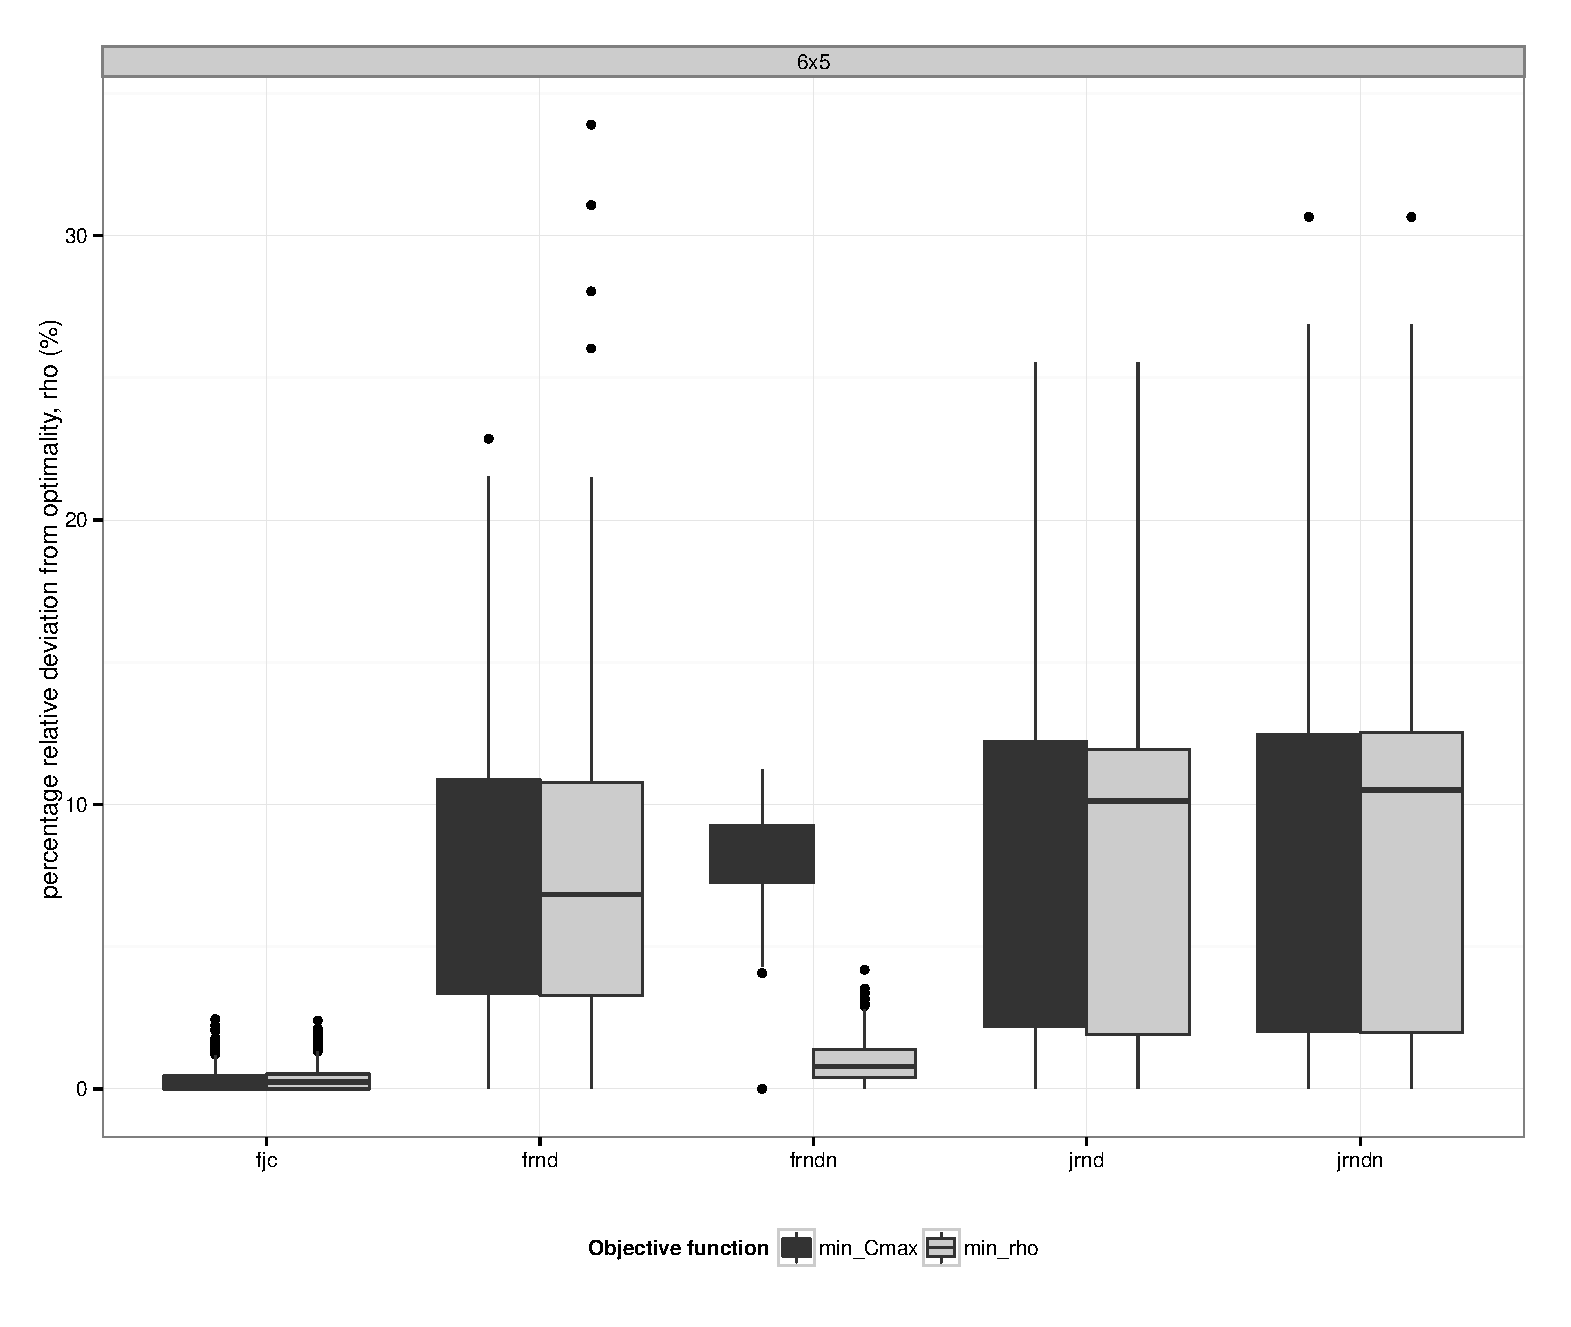
\includegraphics[width=\columnwidth]{CMAboxplotEvoTrain}
\caption{Box-plot of training data for percentage relative deviation from optimality, defined by \cref{eq:rho}, when implementing the final weights obtained from CMA-ES optimisation, using both objective functions from \cref{eq:cma:makespan,eq:cma:rho}, left and right, respectively.}\label{fig:cma:trainboxpl}
\end{figure}

\subsection{Problem difficulty}\label{sec:expr:data}
The evolution of fitness per generation from the CMA-ES optimisation of \cref{eq:cma:rho} is depicted in \cref{fig:cma:fit}, and since all problem spaces reached their allotted computational time, without converging. In fact \frnd{6}{5} and \jrndn{6}{5} needed restarting during the optimisation process. 
Furthermore, the  evolution of the decision variables, $\vec{w}$, are depicted in \cref{fig:cma:wei}. As one can see, the relative contribution for each weight clearly differs between problem spaces. Note that in the case of \jrndn{6}{5} (cf. \cref{fig:cma:wei:rho}), CMA-ES restarts around generation 1,000 and quickly converges back to its previous fitness, however lateral relation of weights has completely changed. Implying that there are many optimal combinations of weights to be used, which can be expected due  to the fact some features in \cref{tbl:features} are a linear combination of one others, e.g., $\phi_3=\phi_1+\phi_2$.

\begin{figure} 
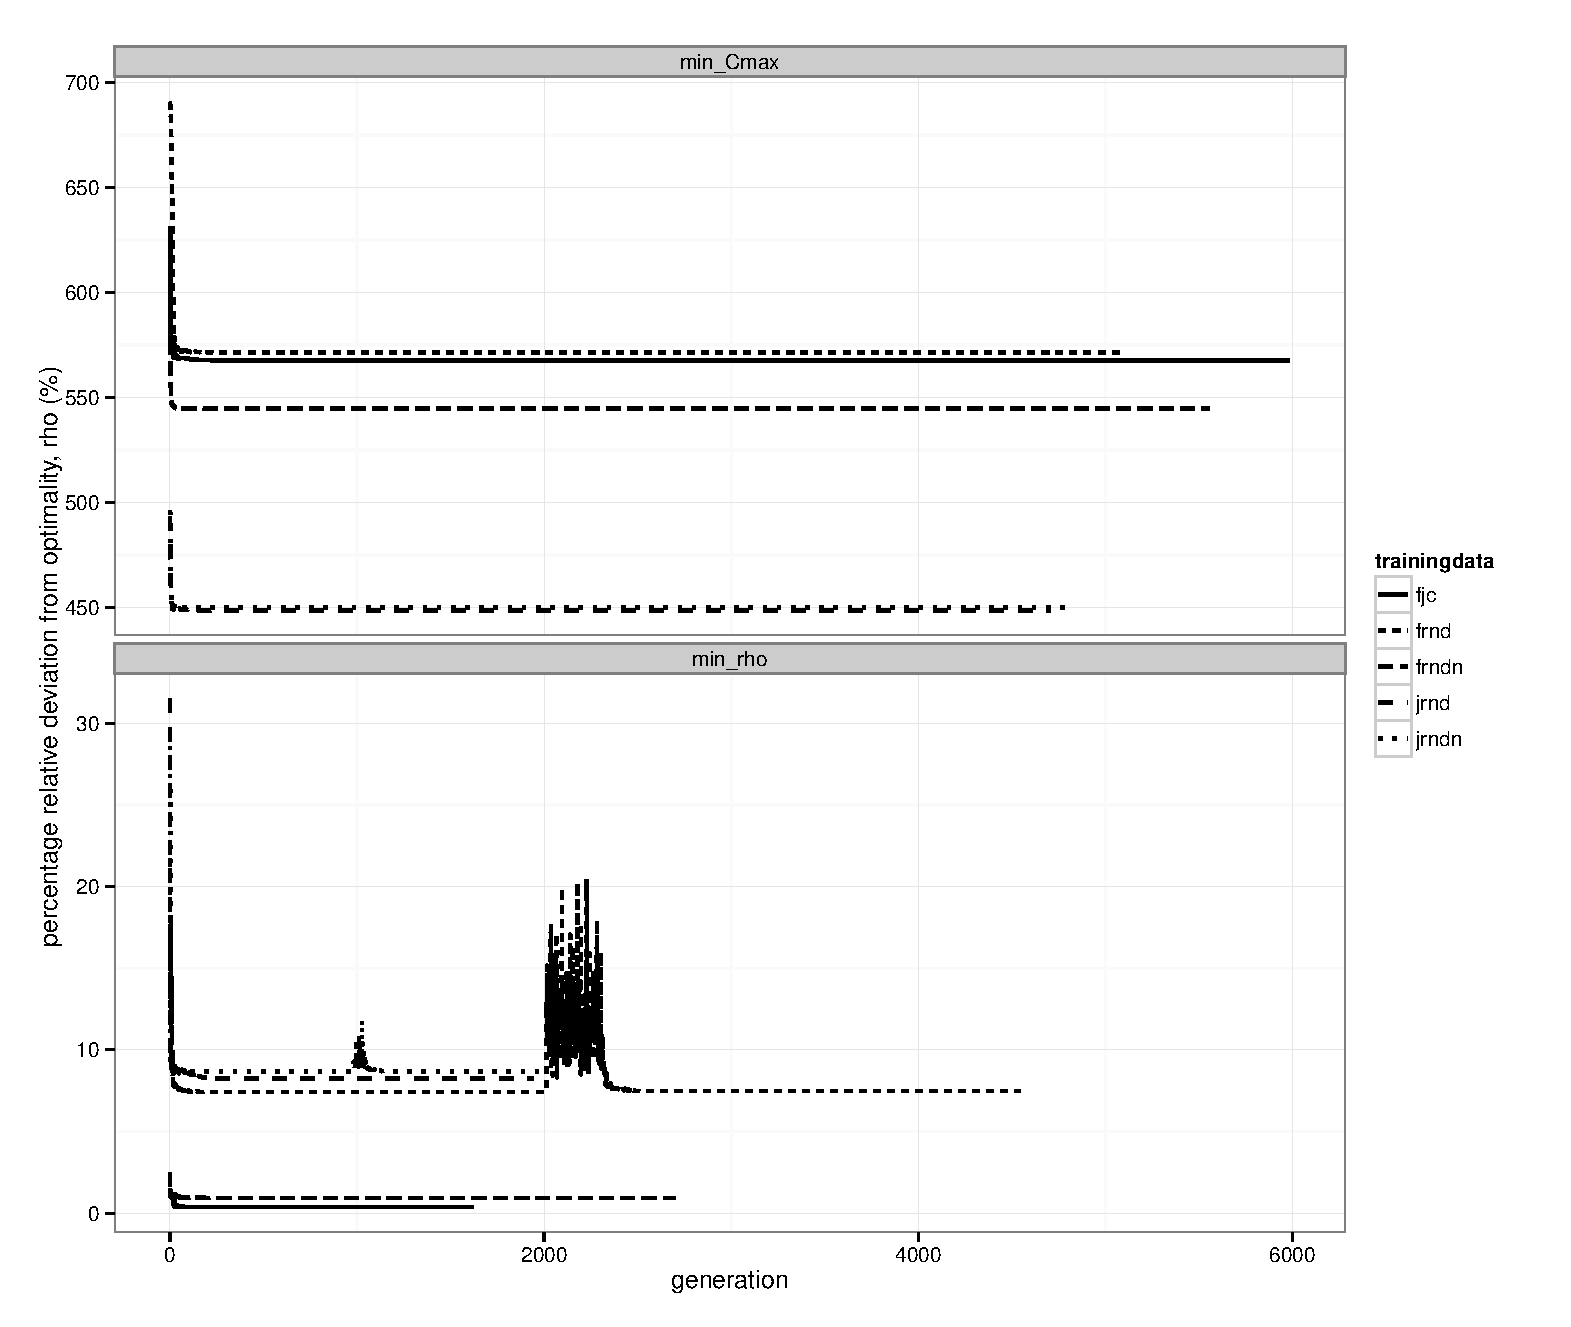
\includegraphics[width=\columnwidth]{CMAfitnessEvo}
\caption{Fitness for optimising (w.r.t. \cref{eq:cma:makespan,eq:cma:rho} above and below, receptively), per generation of the CMA-ES optimisation.}\label{fig:cma:fit}
\end{figure}

\begin{figure*} 
\subcaptionbox{minimise w.r.t. \cref{eq:cma:makespan}}{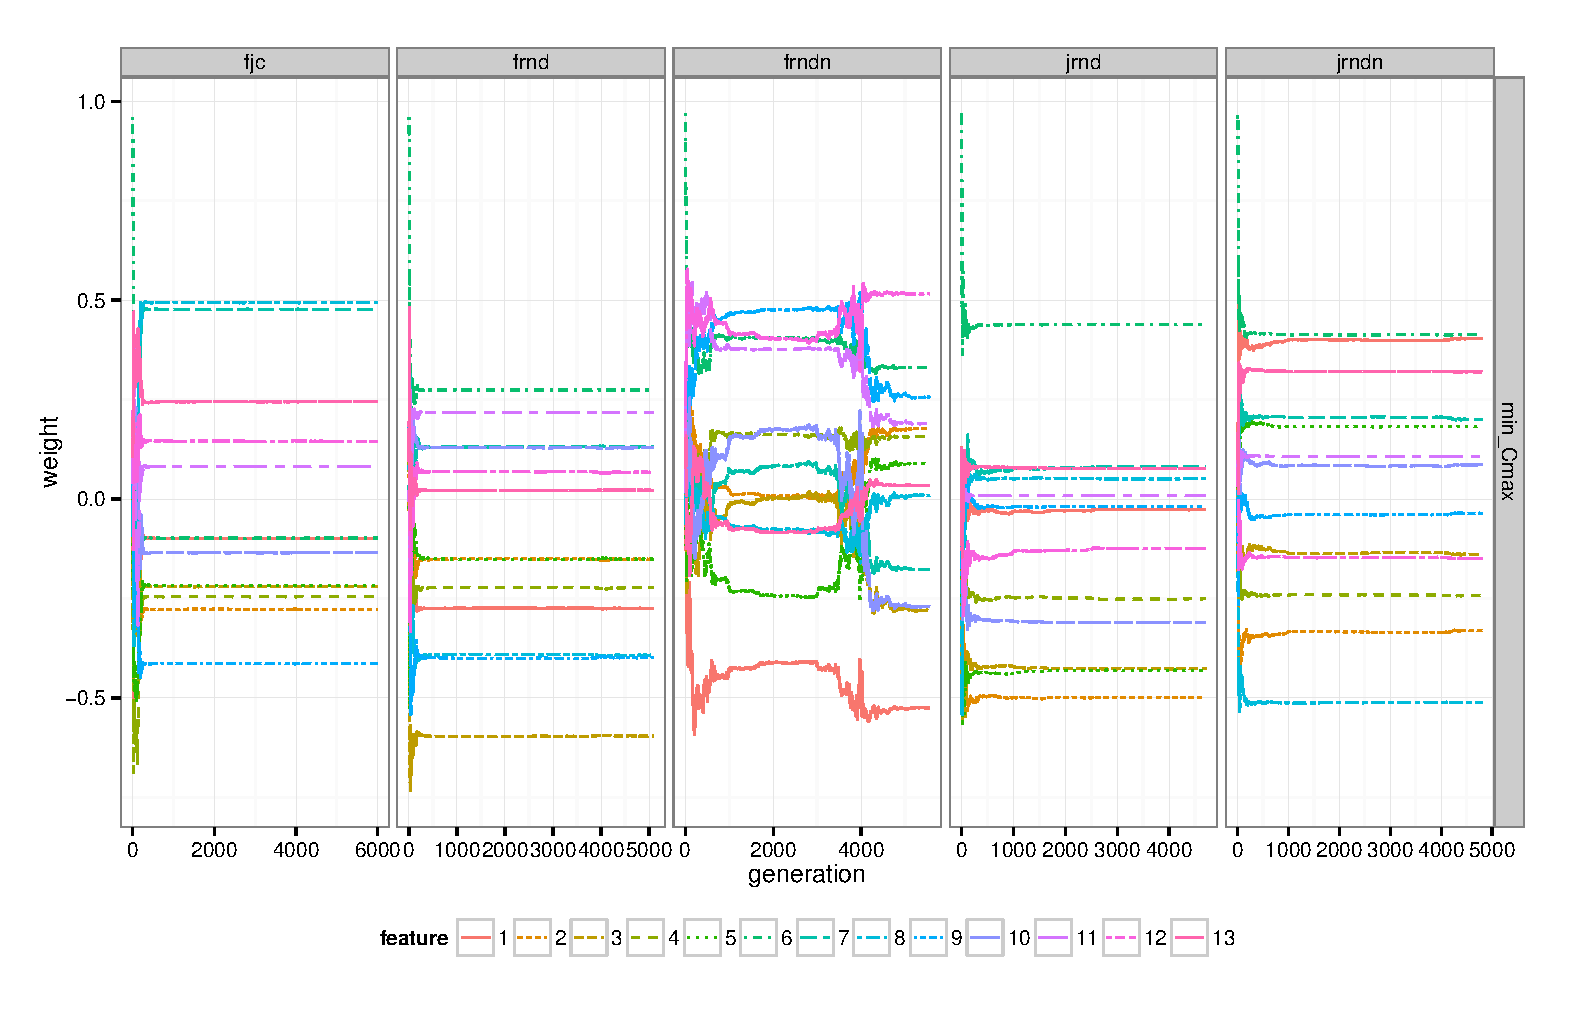
\includegraphics[width=\columnwidth]{CMAweightsEvomin_Cmax}\label{fig:cma:wei:cmax}}
\\
\subcaptionbox{minimise w.r.t. \cref{eq:cma:rho}}{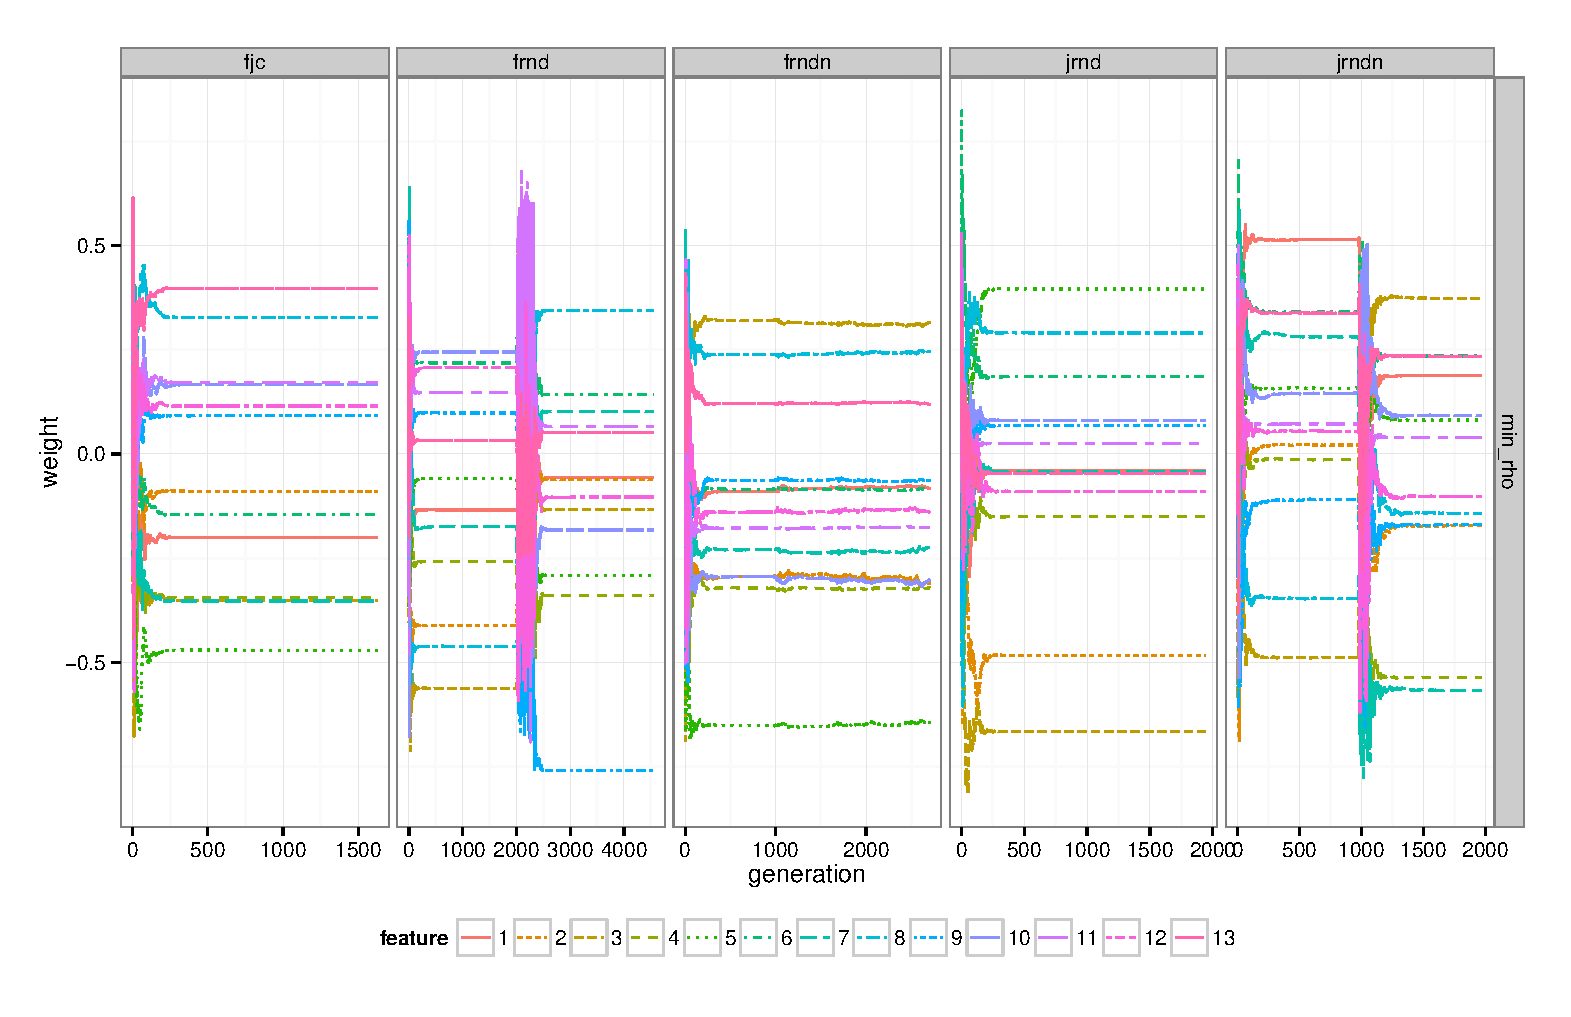
\includegraphics[width=\columnwidth]{CMAweightsEvomin_rho}\label{fig:cma:wei:rho}}
\caption{Evolution of weights of features (given in \cref{tbl:features}) at each generation of the CMA-ES optimisation. Note, weights are normalised such that $\norm{\vec{w}}=1$.}\label{fig:cma:wei}
\end{figure*}


\subsection{Robustness and  scalability}\label{sec:expr:robust} 
As a benchmark, the linear ordinal regression model (PREF) from \cite{InRu11a} was created.
Using the weights obtained from optimising \cref{eq:cma:rho} and applying them on their  $6\times5$ training data, their main statistics of \cref{eq:rho} are reported in \cref{tbl:results:train}, for all training sets described in \cref{tbl:data}. Moreover, the best SDR, from which the features in \cref{tbl:features} were inspired by, are also reported for comparison, i.e., most work remaining (MWR) for all \JSP\ problem spaces, and least work remaining (LWR) for all \FSP\ problem spaces.

To explore the scalability of the learning methods, a similar comparison to \cref{sec:expr:robust} is made for the applying the learning models on their corresponding $10\times10$ testing data, results are reported in \cref{tbl:results:test}. Note that only resulting $C_{\max}$ is reported, as the optimum makespan is not known. 

{\setlength{\tabcolsep}{3pt}
\begin{table}[p]\centering
\caption{Main statistics of percentage relative deviation from optimality, $\rho$, defined by \cref{eq:rho} for various models, using corresponding $6\times5$ training data.}
\label{tbl:results:train}
%jsp
\subfloat[][\jrnd{6}{5}]{\label{tbl:train:j.rnd}
\begin{tabular}{lrrrrr} \toprule
model&mean & med & sd & min & max \\   \midrule
ES$_{C_{\max}}$& 8.54 & 10 &  6 &  0 & 26   \\ % CMA-ES min_Cmax j.rnd 6x5 train
ES$_\rho$& 8.26 & 10 &  6 &  0 & 26   \\ % CMA-ES min_rho j.rnd 6x5 train
PREF&   10.18 & 11 &  7 &  0 & 30  \\ %PREF j.rnd 6x5 train
MWR &  16.48 & 16 &  9 &  0 & 45   \\ %MWR j.rnd 6x5 train
\bottomrule \end{tabular}}
\quad
\subfloat[][\jrndn{6}{5}]{\label{tbl:train:j.rndn}
\begin{tabular}{lrrrrr} \toprule
model&mean & med & sd & min & max \\   \midrule
ES$_{C_{\max}}$& 8.68 & 11 &  6 &  0 & 31   \\ % CMA-ES min_Cmax j.rndn 6x5 train
ES$_\rho$& 8.69 & 11 &  6 &  0 & 31   \\ % CMA-ES min_rho j.rndn 6x5 train
PREF&  10.00 & 11 &  6 &  0 & 31   \\ %PREF j.rndn 6x5 train
MWR &  14.02 & 13 &  8 &  0 & 37   \\ %MWR j.rndn 6x5 train
\bottomrule \end{tabular}}
\\
%flow shop
\subfloat[][\frnd{6}{5}]{\label{tbl:train:f.rnd}
\begin{tabular}{lrrrrr} \toprule
model&mean & med & sd & min & max \\   \midrule
ES$_{C_{\max}}$& 7.44 &  7 &  5 &  0 & 23   \\ % CMA-ES min_Cmax f.rnd 6x5 train
ES$_\rho$& 7.48 &  7 &  5 &  0 & 34   \\ % CMA-ES min_rho f.rnd 6x5 train
PREF&   9.87 &  9 &  7 &  0 & 38  \\ %PREF f.rnd 6x5 train
LWR &  20.05 & 19 & 10 &  0 & 71   \\ %LWR f.rnd 6x5 train
\bottomrule \end{tabular}}
\quad
\subfloat[][\frndn{6}{5}]{\label{tbl:train:f.rndn}
\begin{tabular}{lrrrrr} \toprule
model&mean & med & sd & min & max \\   \midrule
ES$_{C_{\max}}$& 8.09 &  8 &  2 &  0 & 11   \\ % CMA-ES min_Cmax f.rndn 6x5 train
ES$_\rho$& 0.94 &  1 &  1 &  0 &  4   \\ % CMA-ES min_rho f.rndn 6x5 train
PREF&   2.38 &  2 &  1 &  0 &  7  \\ %PREF f.rndn 6x5 train
LWR &  2.25 &  2 &  1 &  0 &  7   \\ %LWR f.rndn 6x5 train
\bottomrule \end{tabular}}
\\
\subfloat[][\fjc{6}{5}]{\label{tbl:train:f.jc}
\begin{tabular}{lrrrrr} \toprule
model&mean & med & sd & min & max \\   \midrule
ES$_{C_{\max}}$& 0.33 &  0 &  0 &  0 &  2   \\ % CMA-ES min_Cmax f.jc 6x5 train
ES$_\rho$& 0.36 &  0 &  0 &  0 &  2   \\ % CMA-ES min_rho f.jc 6x5 train
PREF&   1.08 &  1 &  1 &  0 &  5  \\ %PREF f.jc 6x5 train
LWR &  1.13 &  1 &  1 &  0 &  6   \\ %LWR f.jc 6x5 train
\bottomrule \end{tabular}}
\end{table}

\begin{table}[p]\centering
\caption{Main statistics of $C_{\max}$ for various models, using corresponding $10\times 10$ test data.}
\label{tbl:results:test}
%jsp
\subcaptionbox{\jrnd{10}{10}}{\label{tbl:test:j.rnd}
\begin{tabular}{lrrrrr}  \toprule
model&mean & med & sd & min & max \\ 
  \midrule
ES$_{C_{\max}}$& 922.51 & 914 & 73 & 741 & 1173   \\ % CMA-ES min_Cmax j.rnd 10x10 test
ES$_\rho$& 931.37 & 931 & 71 & 735 & 1167   \\ % CMA-ES min_rho j.rnd 10x10 test
  PREF&   1011.38 & 1004 & 82 & 809 & 1281 \\   %PREF j.rnd 10x10 test
  MWR &  997.01 & 992 & 81 & 800 & 1273   \\ %MWR j.rnd 10x10 test
\bottomrule \end{tabular}}
\quad
\subcaptionbox{\jrndn{10}{10}}{\label{tbl:test:j.rndn}
\begin{tabular}{lrrrrr} \toprule
model& mean & med & sd & min & max \\ 
  \midrule
ES$_{C_{\max}}$& 855.85 & 857 & 50 & 719 & 1010   \\ % CMA-ES min_Cmax j.rndn 10x10 test
ES$_\rho$& 855.91 & 856 & 51 & 719 & 1020   \\ % CMA-ES min_rho j.rndn 10x10 test
  PREF&   899.94 & 898 & 56 & 769 & 1130  \\ %PREF j.rndn 10x10 test
  MWR&  897.39 & 898 & 56 & 765 & 1088   \\ %MWR j.rndn 10x10 test
\bottomrule \end{tabular}}
\\
%flow shop
\subcaptionbox{\frnd{10}{10}}{\label{tbl:test:f.rnd}
\begin{tabular}{lrrrrr} \toprule
model&mean & med & sd & min & max \\   \midrule
ES$_{C_{\max}}$& 1178.73 & 1176 & 80 & 976 & 1416   \\ % CMA-ES min_Cmax f.rnd 10x10 test
ES$_\rho$& 1181.91 & 1179 & 80 & 984 & 1404   \\ % CMA-ES min_rho f.rnd 10x10 test
PREF&  1215.20 & 1212 & 80 & 1006 & 1450  \\ %PREF f.rnd 10x10 test
LWR &  1284.41 & 1286 & 85 & 1042 & 1495   \\ %LWR f.rnd 10x10 test
\bottomrule \end{tabular}}
\quad 
\subcaptionbox{\frndn{10}{10}}{\label{tbl:test:f.rndn}
\begin{tabular}{lrrrrr} \toprule
model&mean & med & sd & min & max \\   \midrule
ES$_{C_{\max}}$& 1065.48 & 1059 & 32 & 992 & 1222   \\ % CMA-ES min_Cmax f.rndn 10x10 test
ES$_\rho$& 980.11 & 980 &  8 & 957 & 1006   \\ % CMA-ES min_rho f.rndn 10x10 test
PREF&  987.49 & 988 &  9 & 958 & 1011  \\ %PREF f.rndn 10x10 test
LWR &  986.94 & 987 &  9 & 959 & 1010   \\ %LWR f.rndn 10x10 test
\bottomrule \end{tabular}}
\\
\subcaptionbox{\fjc{10}{10}}{\label{tbl:test:f.jc}
\begin{tabular}{lrrrrr} \toprule
model&mean & med & sd & min & max \\   \midrule
ES$_{C_{\max}}$& 1135.44 & 1134 & 286 & 582 & 1681   \\ % CMA-ES min_Cmax f.jc 10x10 test
ES$_\rho$& 1135.47 & 1134 & 286 & 582 & 1681   \\ % CMA-ES min_rho f.jc 10x10 test
PREF&   1136.02 & 1135 & 286 & 582 & 1685 \\  %PREF f.jc 10x10 test
LWR &  1136.49 & 1141 & 287 & 581 & 1690   \\ %LWR f.jc 10x10 test
\bottomrule \end{tabular}}
\end{table}}

\section{Discussion and conclusions}\label{sec:disc}
Data distributions considered in this study either varied 
w.r.t. the processing times distributions, continuing the preliminary experiments in  \cite{InRu11a} , or 
w.r.t. the job ordering permutations, i.e., homogeneous $\sigma$ matrices in \FSP\ versus heterogeneous $\sigma$ matrices in \JSP . 
From the results based on $6\times5$ training data, given  in \cref{tbl:results:train}, it's obvious that CMA-ES optimisation substantially outperforms the previous PREF methods from \cite{InRu11a}, for all problem spaces considered. Furthermore, the results hold when testing on $10\times10$, (cf. \cref{tbl:results:test}), suggesting the method is indeed  scalable for higher dimensions. 

Moreover, the study showed that the choice of objective function  for evolutionary search is worth investigating. There was no statistical difference from minimising the fitness function directly and its normalisation w.r.t. true optimum (cf. \cref{eq:cma:makespan,eq:cma:rho}), save for \frndn{6}{5}. Implying, even though ES doesn't rely on optimal solutions, there are some problem spaces where it can be of great benefit. This is due to the fact that the problem instances can vary greatly within the same problem space \cite{InRu12}, thus normalising the objective function would help the evolutionary search to deviate the from giving too much weight for problematic problem instances for the greater good.

The weights for \cref{eq:jssp:linweights} in \cite{InRu11a} were found using supervised learning, where the training data was created from optimal solutions of randomly generated problem instances. As an alternative, this study showed  that minimising the mean makespan directly using a brute force search via CMA-ES actually results in a better CDRs. The nature of CMA-ES is to explore suboptimal routes until it converges to an optimal one. Implying that the previous approach of only looking into one optimal route may not produce a sufficiently rich training set. That is, the training set should incorporate a more complete knowledge on \emph{all} possible preferences, i.e., make also the distinction between suboptimal and sub-suboptimal features, etc.  This would require a Pareto ranking of preferences which can be used to make the distinction to which feature sets are equivalent, better or worse -- and to what degree, i.e., by giving a weight to the preference. This would result in a very large training set, which of course could be re-sampled in order to make it computationally feasible to learn.

The main drawback of using evolutionary search for learning optimal weights for \cref{eq:jssp:linweights} is how computationally expensive it is to evaluate the mean expected fitness. Even for a low problem dimension, 6-job 5-machine \JSP , each optimisation run reached their walltime of 288hrs, without converging. Now, $6\times5$ \JSP\ requires 30 sequential dispatches, where at each time step there are up to $6$ jobs to choose from, i.e., its complexity is $\mathcal{O}(n^{n\cdot m})$, making it computationally infeasible to apply this framework for higher dimensions as is. 
However, evolutionary search only requires the rank of the candidates, and therefore it is appropriate to retain a sufficiently accurate surrogate for the value function during evolution in order to reduce the number of costly true value function evaluations, such as the approach in \cite{InRu11b}. This could reduce the computational cost of the evolutionary search considerably, making it feasible to conduct the experiments from \cref{sec:es:measure} for problems of higher dimensions, e.g., with these adjustments it is possible to train on $10\times10$ and test on for example $14\times14$ to verify whether scalability holds for even higher dimensions.  






\HeaderQuote{The adventures first... explanations take such a dreadful time.}{The Gryphon} %Alice's Adventures in Wonderland:


\chapter{Experiments }\label{ch:experiments} 
\todoWrite{Compare CMA-ES to PREF models}

\FirstSentence{T}{here's something to be said} for having a good opening line. Morbi commodo, ipsum sed pharetra gravida, orci  $x = 1/\alpha$ magna rhoncus neque, id pulvinar odio lorem non turpis. Nullam sit amet enim. Suspendisse id velit vitae ligula volutpat condimentum. Aliquam erat volutpat. Sed quis velit. Nulla facilisi. Nulla libero. Vivamus pharetra posuere sapien. Nam consectetuer. Sed aliquam, nunc eget euismod ullamcorper, lectus nunc ullamcorper orci, fermentum bibendum enim nibh eget ipsum. Donec porttitor ligula eu dolor. Maecenas vitae nulla consequat libero cursus venenatis. Nam magna enim, accumsan eu, blandit sed, blandit a, eros.
$$\zeta = \frac{1039}{\pi}$$

\HeaderQuote{Tut, tut, child! Everything's got a moral, if only you can find it.}{The Duchess} 

\chapter{Conclusions}\label{ch:conclusions} 
\todoWrite{Write overall conclusions of dissertation!}

\FirstSentence{L}{orem ipsum dolor sit amet}, consectetuer adipiscing elit. Morbi commodo, ipsum sed pharetra gravida, orci magna rhoncus neque, id pulvinar odio lorem non turpis. Nullam sit amet enim. Suspendisse id velit vitae ligula volutpat condimentum. Aliquam erat volutpat. Sed quis velit. Nulla facilisi. Nulla libero. Vivamus pharetra posuere sapien. Nam consectetuer. Sed aliquam, nunc eget euismod ullamcorper, lectus nunc ullamcorper 





The analysis-phase of \Alice\ is heavily dependent on having an expert 
policy one wants to mimic, i.e., knowing the \emph{optimal} solutions for the 
sake of imitation learning. 

Understandably, knowing the true optimum is an unreasonable claim in many 
situations, especially for high dimensional problem instances. 
Luckily, there seems to be the possibility to circumvent querying the expert 
altogether, and still have reasonable performance. 
By applying \emph{locally optimal learning to search} \citep{ChangKADL15} it is 
possible to use imitation learning even when the reference policy is poor. 
Although it's noted that the quality (w.r.t near-optimality) of reference 
policy is in accordance to its performance, as is to be expected. 



% Back matter
\printBackMatter{\printAll}


\end{document}
